%-------------------------------------------------------------------------------
%                      Template Naskah Skripsi
%               	Berdasarkan format JTETI FT UGM
% 						(c) @gunturdputra 2014
%-------------------------------------------------------------------------------

%Template pembuatan naskah skripsi.
\documentclass{jtetiskripsi}

%Untuk prefiks pada daftar gambar dan tabel
\usepackage[titles]{tocloft}
\renewcommand\cftfigpresnum{Gambar\  }
\renewcommand\cfttabpresnum{Tabel\   }

%Untuk hyperlink dan table of content
\usepackage[hidelinks]{hyperref}
\newlength{\mylenf}
\settowidth{\mylenf}{\cftfigpresnum}
\setlength{\cftfignumwidth}{\dimexpr\mylenf+2em}
\setlength{\cfttabnumwidth}{\dimexpr\mylenf+2em}

%Untuk Bold Face pada Keterangan Gambar
\usepackage[labelfont=bf]{caption}

%Untuk caption dan subcaption
\usepackage{caption}
\usepackage{subcaption}

%pdf
\usepackage{pdfpages}

%table
\usepackage{graphics}

\usepackage{wrapfig}

%bibliography
\usepackage{natbib}

%equation
\usepackage{amsmath}
\usepackage{amsfonts}

%algoritma
\usepackage{algorithm}
\usepackage{algpseudocode}

%listing
\usepackage{listings}

%table
\usepackage{array}

%-----------------------------------------------------------------
%Disini awal masukan untuk data proposal skripsi
%-----------------------------------------------------------------
\titleind{\emph{Automatic Tagging dengan Menggunakan Algoritma Bipartite Graph Partition dan Two Way Poisson Mixture Model}}

\fullname{Muhammad Zhafran Bahij}

\idnum{1313619012}

%\approvaldate{12 Februari 2019}
\approvaldate{.. ... 2023}

\degree{Sarjana Ilmu Komputer}

\yearsubmit{2023}

\program{Ilmu Komputer}

\dept{Ilmu Komputer}

\firstsupervisor{Muhammad Eka Suryana, M. Kom.}
\firstnip{198512232012121002}

\secondsupervisor{Med Irzal, M. Kom.}
\secondnip{198512232012121002}

%-----------------------------------------------------------------
%Disini akhir masukan untuk data proposal skripsi
%-----------------------------------------------------------------

\tolerance=1
\emergencystretch=\maxdimen
\hyphenpenalty=10000
\hbadness=10000

\begin{document}

\cover

% \chapter*{\centering{\large{LEMBAR PENGESAHAN}}}
\thispagestyle{empty} {\bf }Dengan ini saya mahasiswa Fakultas
Matematika dan Ilmu Pengetahuan Alam, Universitas Negeri Jakarta

\vskip3mm

\begin{tabular}{ll}
  Nama & : Muhammad Zhafran Bahij \\
  No. Registrasi & : 1313619012\\
  Program Studi & : Ilmu Komputer \\
  Judul & : Automatic Tagging dengan Menggunakan Algoritma \\ & \hspace{0.2cm} Bipartite Graph Partition dan Two Way Poisson Mixture \\ & \hspace{0.2cm} Model
%  Judul & : Pengaruh Penggunaan \emph{Color Model} LAB dan HLS dalam \\ & \hspace{0.2cm} Kalibrasi Warna Luka Menggunakan Metode Segmentasi \\ & \hspace{0.2cm} \emph{K-Means} dan \emph{Mean Shift}\\
\end{tabular}

\vskip3mm

\noindent \hskip10mm 
% Menyatakan bahwa proposal ini telah siap diajukan untuk sidang skripsi.
\begin{center}
Menyatakan bahwa skripsi ini telah siap diajukan untuk sidang skripsi.
\end{center}



\begin{center}
\vskip3mm

Menyetujui,

\vskip3mm
\begin{spacing}{1.25}

\begin{tabular}{ccc}
  \hskip-2mm Dosen Pembimbing I & \qquad \qquad \qquad \qquad & \hskip-6mm Dosen Pembimbing II \\
   &  &  \\
   &  &  \\
   &  &  \\
   &  &  \\
  \hskip-2mm \underline{\textbf{Muhammad Eka Suryana, M. Kom}} &  & \hskip-6mm \underline{\textbf{Med Irzal, M.Kom.}} \\
  \hskip-2mm NIP. 19851223 201212 1 002 &  & \hskip-6mm NIP. 19770615 200312 1 001	 \\
\end{tabular}
\end{spacing}
\end{center}
\vskip3mm
\begin{center}
Mengetahui, \\
Koordinator Program Studi Ilmu Komputer
\end{center}
\begin{spacing}{1.25}
{ \ }
\\
\\
{ \ }\begin{center}
\underline{\textbf{Dr. Ria Arafiyah, M.Si.}} \\
{NIP. 19751121 200501 2 004}
\end{center}
\end{spacing} 
% \addcontentsline{toc}{chapter}{LEMBAR PERSETUJUAN}
\chapter*{\centering{\large{\thesisapprovalname}}}
\thispagestyle{empty} {\bf }
\vspace{-0.5cm}
\begin{center}
	\textbf{\textit{Automatic Tagging} dengan Menggunakan Algoritma \textit{Bipartite Graph Partition} dan \textit{Two Way Poisson Mixture Model}}
\end{center}

\vspace{1mm}
\vskip 1.5mm \noindent
\begin{tabular}{ll}
	\hskip-2mm Nama & : Muhammad Zhafran Bahij \\
	\hskip-2mm No. Registrasi & : 1313619012 \\
\end{tabular}


\vskip2mm

\noindent \begin{flushleft}
	\begin{tabular}{llcc}
		
		& \hskip15mm \textbf{Nama} & \textbf{Tanda Tangan} & \textbf{Tanggal} \\
		
		\hskip-1cm \textbf{Penanggung Jawab} &  &  &  \\
		\hskip-1cm Dekan & : Prof. Dr. Muktiningsih N, M.Si. & ............... & ............. \\
		& \hskip3mm NIP. 196405111989032001 &  &  \\
		\hskip-1cm \textbf{Wakil Penanggung Jawab} &  &  &  \\
		\hskip-1cm Wakil Dekan Bidang Akademik & : Dr. Esmar Budi, S.Si., MT. & ............... & ............. \\
		& \hskip3mm NIP. 197207281999031002 &  &  \\
		\hskip-1cm Ketua & : Ir. Fariani Hermin Indiyah, MT. & ............... & ............. \\
		& \hskip3mm NIP. 196605171994031003 &  &  \\
		\hskip-1cm Sekretaris & : Ari Hendarno, S.Pd, M.Kom & ............... & ............. \\
		& \hskip3mm NIP. 198811022022031002 &   &  \\	
		\hskip-1cm Penguji Ahli & : Dr. Ria Arafiyah, M.Si. & ............... & ............. \\
		& \hskip3mm NIP. 197511212005012004 &  &  \\
		\hskip-1cm Pembimbing I & : Muhammad Eka Suryana, M.Kom. & ............... & ............. \\
		& \hskip3mm NIP. 198512232012121002 &  &  \\		
		\hskip-1cm Pembimbing II & : Med Irzal, M.Kom. & ............... & ............. \\
		& \hskip3mm NIP. 197706152003121001 &  &  \\
	\end{tabular}
\end{flushleft}

\vskip1mm

\noindent \textbf{Dinyatakan lulus ujian skripsi tanggal: 22 Agustus 2023}


% \addcontentsline{toc}{chapter}{LEMBAR PERNYATAAN}
\chapter*{\centering{\large{LEMBAR PERNYATAAN}}}

Saya menyatakan dengan sesungguhnya bahwa skripsi dengan judul	\textbf{\textit{Automatic Tagging} dengan Menggunakan Algoritma \textit{Bipartite Graph Partition} dan \textit{Two Way Poisson Mixture Model}} yang disusun sebagai syarat untuk memperoleh gelar Sarjana komputer dari Program Studi Ilmu Komputer Universitas Negeri Jakarta adalah karya ilmiah saya dengan arahan dari dosen pembimbing.

Sumber informasi yang diperoleh dari penulis lain yang
telah dipublikasikan yang disebutkan dalam teks skripsi ini, telah dicantumkan dalam Daftar Pustaka sesuai dengan norma, kaidah dan etika penulisan ilmiah.

Jika dikemudian hari ditemukan sebagian besar skripsi ini bukan hasil karya saya sendiri dalam bagian-bagian tertentu, saya bersedia menerima sanksi pencabutan gelar akademik yang saya sanding dan sanksi-sanksi lainnya sesuai dengan peraturan perundang-undangan yang berlaku.

\vspace{.5cm}

\begin{tabular}{p{7.5cm}c}
	&Jakarta, 10 Agustus 2023\\
	&\\
	&\\
	&\\
	&Muhammad Zhafran Bahij
\end{tabular}

%-----------------------------------------------------------------
%Disini awal masukan Acknowledment
%-----------------------------------------------------------------
% \acknowledgment
% \begin{flushright}
% 	\emph{Untuk Ayah dan Ibu.}
% \end{flushright}
%-----------------------------------------------------------------
%Disini awal masukan untuk Prakata
%-----------------------------------------------------------------
\preface

Ungkapan Puji dan Syukur penulis panjatkan kehadirat Tuhan Yang Maha Esa, atas segala rahmat dan karunia-Nya sehingga penulis dapat menyelesaikan skripsi ini dengan baik. Adapun jenis penelitian yang dengan judul \textit{Automatic Tagging dengan Menggunakan Algoritma Bipartite Graph Partition dan Two Way Poisson Mixture Model}

Dalam menyelesaikan skripsi ini, penulis selalu mendapat dorongan dan bantuan. Oleh karena itu, penulis menyampaikan terima kasih kepada:

\begin{enumerate}
  \item Para petinggi di lingkungan FMIPA Universitas Negeri Jakarta.
  \item Ibu Dr. Ria Arafiyah, M.Si. selaku Koordinator Program Studi Ilmu Komputer.
  \item Bapak Muhammad Eka Suryana, M.Kom. selaku Dosen Pembimbing I yang telah membimbing, mengarahkan, serta memberikan saran dan koreksi terhadap skripsi ini.
  \item Bapak Med Irzal M.Kom. selaku Dosen Pembimbing II yang telah membimbing, mengarahkan, serta memberikan saran dan koreksi terhadap skripsi ini.
  \item Ayah dan Ibu penulis yang selama ini telah mendukung penulis dalam menyelesaikan skripsi ini dalam berbagai hal.
  \item Sepupu penulis yang telah menginspirasi penulis untuk menjalani kehidupan di Program Studi Ilmu Komputer.
  \item Teman-teman Ilmu Komputer 2019 yang telah menyemangati penulis dalam penulisan skripsi.
  \item Rekan-rekan PT Fhadira Inovasi Teknologi yang telah mendukung penulis untuk menyelesaikan skripsi.
  \item Teman-teman KANAU yang secara tidak langsung melatih penulis agar terbiasa melakukan penulisan.
  \item Kawan-kawan penulis yang tidak bisa disebutkan satu persatu.
\end{enumerate}

Dalam penulisan skripsi ini, penulis menyadari bahwa dengan keterbatasan ilmu dan pengetahuan penulis, skripsi ini masih jauh dari sempurna, baik dari segi penulisan, penyajian materi, maupun bahasa. Oleh karena itu, penulis sangat membutuhkan kritik dan saran yang dapat dijadikan sebagai pembelajaran serta dapat membangun penulis agar lebih baik lagi kedepannya.

Akhir kata, penulis berharap ini bermanfaat bagi semua pihak khususnya penulis sendiri, serta menjadi semangat dan motivasi bagi rekan-rekan yang akan melaksanakan skripsi berikutnya. Semoga Tuhan Yang Maha Esa senantiasa membalas kebaikan semua pihak yang telah membantu penulis dalam menyelesaikan proposal ini.

%\vspace{.5cm}

\begin{tabular}{p{8.5cm}r}
	&Terima kasih,\\
	&Jakarta, 10 Agustus 2023\\
	&\\
	&\\
%	&\\
	&Penulis
\end{tabular}

%-----------------------------------------------------------------
%Disini awal masukan Intisari
%-----------------------------------------------------------------
\begin{abstractind}
\textbf{MUHAMMAD ZHAFRAN BAHIJ}. \emph{Automatic Tagging} dengan Menggunakan Algoritma \emph{Bipartite Graph Partition} dan \emph{Two Way Poisson Mixture Model}. Skripsi. Fakultas Matematika dan Ilmu Pengetahuan Alam, Universitas Negeri Jakarta. 2023. Di bawah bimbingan Muhammad Eka Suryana, M. Kom. dan Med Irzal, M. Kom.
\vskip1cm
  % \textit{Automatic Tagging} merupakan hal yang dilakukan untuk menentukan
  % suatu kata kunci atau frasa kunci yang relevan pada suatu artikel, dokumen, gambar,
  % atau video secara otomatis. Untuk melakukan hal ini diperlukan algoritma
  % \textit{Bipartite Graph Partition} dan \textit{Two Way Poisson Mixture Model}.
  % Penelitian ini merupakan bagian dari

  \textit{Automatic Tagging} merupakan hal yang dilakukan untuk menentukan
  suatu kata kunci atau frasa kunci yang relevan pada suatu artikel, dokumen, gambar,
  atau video secara otomatis. Penelitian ini merupakan salah satu payung penelitian dari
  mesin pencari atau \textit{search engine Telusuri}. Agar bisa melakukan pencarian dengan lebih efisien, salah satu caranya adalah pencarian melalui \textit{tag}. 
  Sebelum mencapai tahap pencarian melalui \textit{tag},
  langkah awal yang diperlukan adalah membuat program \textit{Automatic Tagging}. Dalam penelitian ini, 
  algoritma yang digunakan adalah \textit{Bipartite Graph Partition} dan \textit{Two Way Poisson Mixture Model} dengan
  menggunakan data latih dari suatu \textit{website} \textit{thehill.com}. Proses pembentukkan algoritma tersebut
  menggunakan bahasa pemrograman \textit{Python}. Hasil akhir dari penelitian ini adalah mampu memberikan enam 
  \textit{tag} dengan ketepatan akurasi sebesar 37\% dengan menggunakan data 229 dokumen atau artikel dan 723 \textit{tag}. 
  Hal ini terjadi karena program yang telah dibuat tidak bisa membagi \textit{Bipartite Graph Partition} sebanyak $K$ lebih dari dua.

  
	\bigskip
	\noindent

	\textbf{Kata kunci :} \textit{tagging}, \textit{database}, \textit{bipartite graph}, \textit{Poisson Mixture Model}
\end{abstractind}

\begin{abstracteng}

\textbf {MUHAMMAD ZHAFRAN BAHIJ}. \emph{Automatic Tagging Using Bipartite Graph Partition and Two Way Poisson Mixture Model. Thesis. Faculty of Mathematics and Natural Sciences, State University of Jakarta. 2021. Supervised by} Muhammad Eka Suryana, M. Kom. \emph{and} Med Irzal, M. Kom. 
\vskip1cm

\textit{Automatic Tagging is finding relevant key words or key phrases in article, document, image, and video automatically.
This research is under search engine Telusuri's research. Another way to increase efficiency of Telusuri is searching with tag.
Before do searching with tag, the first step is create an Automatic Tagging. 
Two algorithm to build this program are Bipartite Graph Partition and Two Way Poisson Mixture Model with data from thehill.com . This program created by Python language.
The final result of this research is Automatic Tagging can give six tag with 37\% accuration with 229 document and 723 tag. The accuration is too low because
the program cannot partition the Bipartite Grap Partition with K more than two.
}

\bigskip
\noindent
\textbf {Keywords:} \textit{tagging}, \textit{database}, \textit{bipartite graph}, \textit{Poisson Mixture Model}
\end{abstracteng}
%-----------------------------------------------------------------
%Disini akhir masukan Intisari
%-----------------------------------------------------------------
%-----------------------------------------------------------------

%-----------------------------------------------------------------
%Disini akhir masukan untuk muka skripsi
%-----------------------------------------------------------------

\tableofcontents 
\addcontentsline{toc}{chapter}{DAFTAR ISI}
\listoffigures
\addcontentsline{toc}{chapter}{DAFTAR GAMBAR}
% \listoftables
% \addcontentsline{toc}{chapter}{DAFTAR TABEL}

\begin{counterpage}
\end{counterpage}
%Disini awal masukan untuk Bab
%-----------------------------------------------------------------
%!TEX root = ./template-skripsi.tex
%-------------------------------------------------------------------------------
% 								BAB I
% 							LATAR BELAKANG
%-------------------------------------------------------------------------------

\chapter{PENDAHULUAN}

\section{Latar Belakang Masalah}

Saat ini, penggunaan \textit{search engine} atau mesin pencari telah digunakan oleh khalayak umum untuk mencari berbagai informasi yang ada. Berdasarkan data dari \citep{reliablesoft2022}, Google merupakan \textit{search engine} yang menempati urutan pertama terpopuler, selanjutnya diikuti dengan Bing, Baidu, Yahoo!, Yandex, dan DuckDuckGo.

\begin{figure}[h]
    \centering
    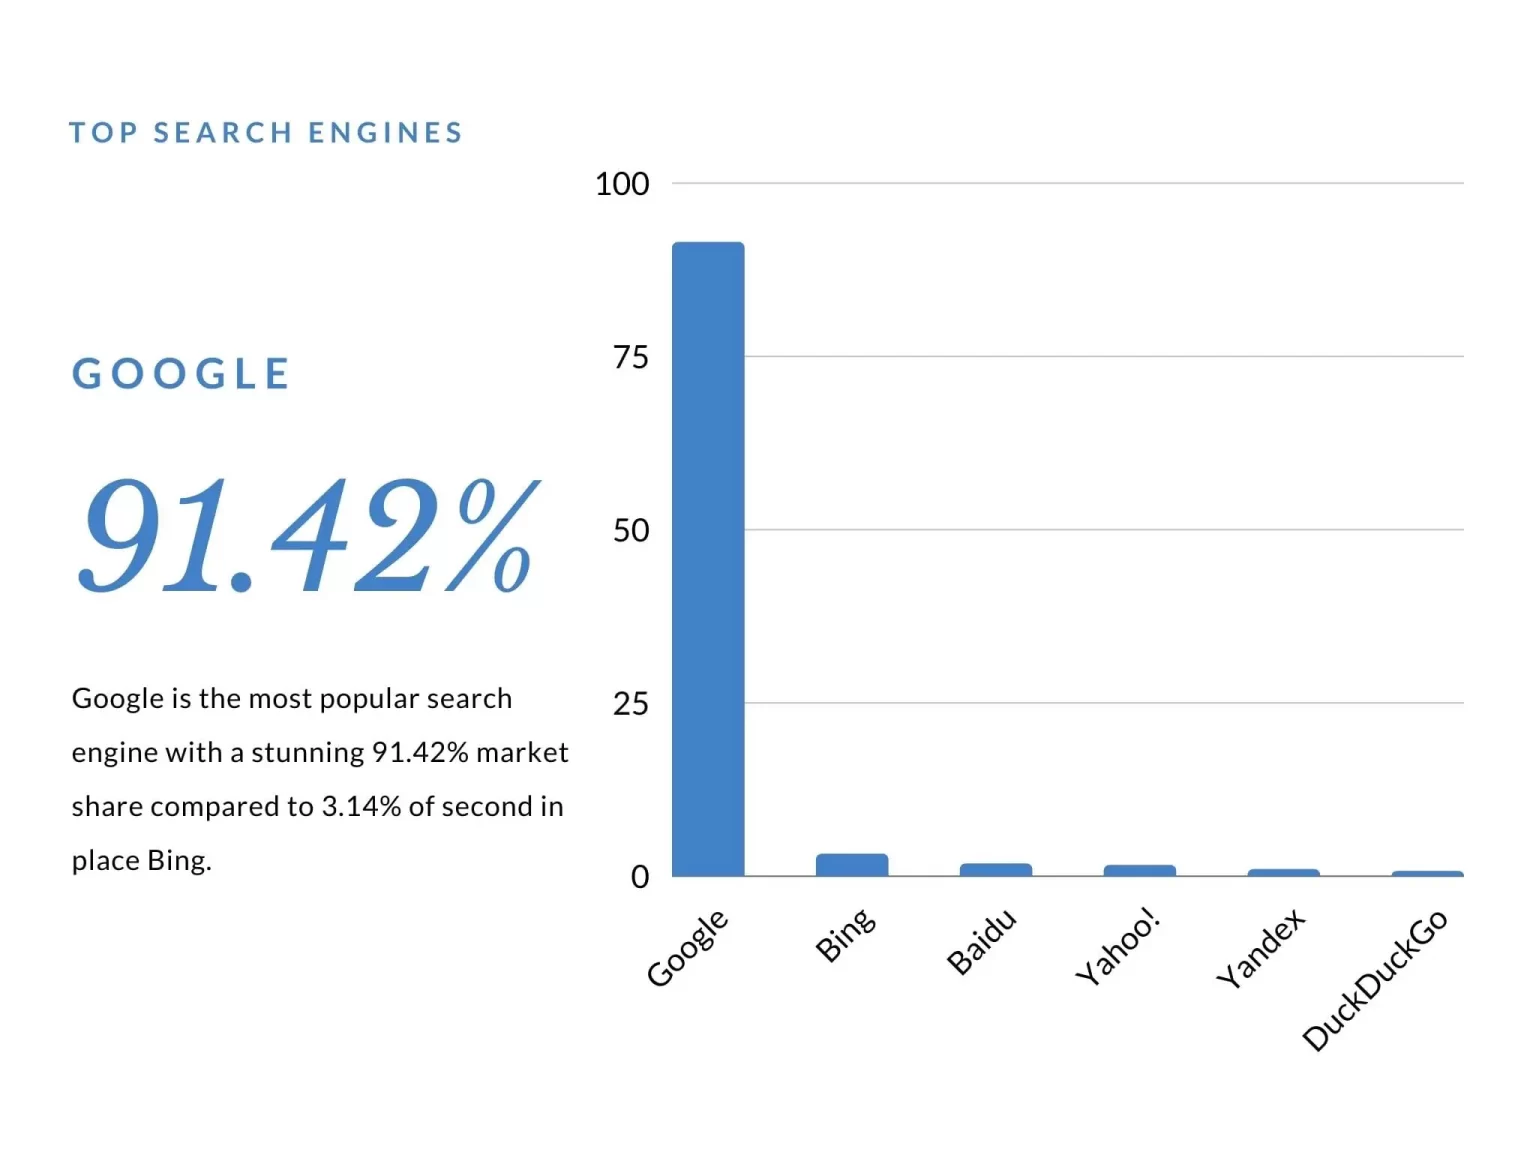
\includegraphics[width=0.75\textwidth]{gambar/Top Search Engine.png}
    \caption{Pengguaan search engine terpopuler \citep{reliablesoft2022}}
    \label{gambar:search_engine_populer}
\end{figure}

\textit{Web Search Engine} atau mesin pencari web merupakan suatu perangkat lunak yang digunakan untuk mencari sesuatu di internet berdasarkan kata-kata yang diberikan oleh pengguna sebagai \textit{search terms}. Pembuatan \textit{search engine} pertama kali dilakukan oleh Alan Emtage, Bill Heelan, dan J. Peter Deutsch pada tahun 1990. Mereka menamai \textit{search engine} tersebut yaitu Archie \citep{seymour2011history}.

Pekerjaan utama dari \textit{search engine} ada tiga yaitu \textit{web crawling, indexing,} dan \textit{searching}. \textit{Search engine} bekerja dengan cara mengirimkan informasi tentang halaman web, Halaman tersebut di dapat dari \textit{web crawler} suatu \textit{automated web browser} yang mengikuti seluruh pranala yang ada di situs. Pengecualian situs yang dicari dapat dilakukan melalui "\textit{robots.txt}". Kemudian, konten dari setiap halaman akan dianalisis untuk menentukan urutan index. Data tentang halaman web dikirim ke dalam \textit{index database} yang nantinya akan dilakukan \textit{query}. \textit{Query} bisa satu kata atau lebih. Tujuan pengindeksan adalah untuk menemukan informasi secepat mungkin \citep{seymour2011history}.

\begin{figure}[h]
    \centering
    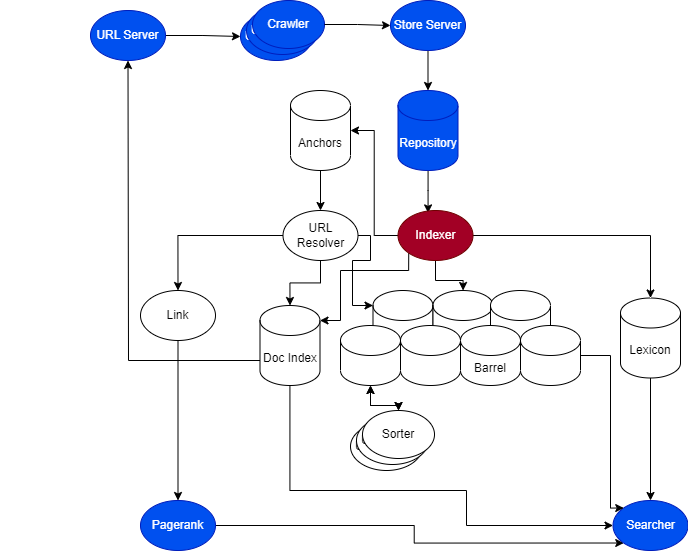
\includegraphics[width=0.75\textwidth]{gambar/Skema Search Engine Google.png}
    \caption{High Level Google Architecture \citep{brin1998anatomy}}
    \label{gambar:high_level_google_architecture}
\end{figure}

Pada Gambar \ref{gambar:search_engine_populer}, telah diperlihatkan bahwa Google merupakan \textit{search engine} terfavorit. Google ditemukan oleh Larry Page dan Sergey Brin pada tahun 1998. Salah satu keunggulan Google adalah pengaplikasian PageRank  yaitu mengatasi \textit{underspecified queries}. Sebagai contohnya, jika kita mencari kata Real Madrid, maka situs pertama kali yang terlihat adalah situs resmi Real Madrid.

Gambar \ref{gambar:high_level_google_architecture} merupakan struktur arsitektur Google. Warna biru menunjukkan hasil penelitian yang dilakukan oleh Lazuardy Khatulistiwa dalam penelitian yang berjudul “Perancangan Arsitektur Search Engine dengan Mengintegrasikan \textit{Web Crawler, Algoritma Page Ranking}, dan \textit{Document Ranking}” dan warna merah menunjukkan proses penelitian dari Zaidan Pratama dalam judul “Perancangan Modul Pengindeks pada \textit{Search Engine} Berupa \textit{Induced Generalized Suffix Tree} untuk Keperluan Perangkingan Dokumen”.
Salah satu komponen dalam \textit{search engine} milik Google adalah \textit{Indexer}. Dalam penelitian Zaidan Pratama, di sana menjelaskan tentang melakukan pengindeksan melalui algoritma \textit{General Suffix Tree} (\textit{GST}) yang termodifikasi. (\cite{pratama2022igst})

% Akan tetapi, penelitian ini memiliki kekurangan yaitu hanya bisa mengambil judul dari suatu dokumen. Beberapa dokumen terkadang tidak memiliki relevansi dengan judulnya dan itu bisa saja menyebabkan masalah sehingga diperlukan adanya tag.

Proses pengindeksan dimulai dengan memasukkan kumpulan dokumen yang dibuat menjadi \textit{GST}. Kemudian, membuat \textit{GST} dari kumpulan dokumen tersebut. Dari \textit{GST} tersebut, nantinya akan dilakukan reduksi untuk node yang redundan atau node yang mengalami perulangan yang tidak diperlukan sehingga akan terbentuk pohon yang terinduksi untuk frekuensi \textit{f} yang bernama \textit{Induced Generalized Suffix Tree-f}. 

\textit{IGST-f}  ini menjadi komponen utama dalam pengindeksan. Setelah itu, program menerima masukan berupa pola kata dan batas \textit{k} untuk dicari pada kumpulan dokumen. Dari sinilah kita akan mencari nilai \textit{count} dari setiap \textit{node}. Kemudian, mencatat jumlah dokumen dalam \textit{sublist} yang tereduksi untuk setiap \textit{node}. Selanjutnya, mencari nilai \textit{counter lowest common ancestor} dari setiap \textit{node}. Terakhir, mengenai Indeks Efisien. Untuk \textit{Top-k Document Retrieval Problem} dilakukan pengurutan terhadap representasi \textit{array IGST-f} yang sudah memiliki nilai \textit{count} dan mengembalikan hasil \textit{top-k} yang meiliki pola \textit{P}. \cite{pratama2022igst}

\begin{figure}[H]
    \centering
    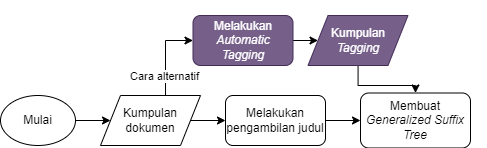
\includegraphics[width=1\textwidth]{gambar/Skema singkat General Suffix Tree.png}
    \caption{Bagian \textit{Automatic Tagging} pada \textit{Indexer}}
    \label{gambar:automatic_tagging}
\end{figure}

Akan tetapi, pengindeksan tersebut masih hanya melalui judul dan belum melalui \textit{tag}. Oleh karena itu, salah satu alternatifnya adalah melakukan pengindeksan melalui \textit{tag}. Pada gambar \ref{gambar:automatic_tagging} Warna ungu adalah salah satu alternatif yang dapat dilakukan yaitu melalui \textit{automatic tagging} yang nantinya peneliti akan lakukan. Hal ini dapat dimanfaatkan agar bisa melakukan pengindeksan lebih akurat.
	
\textit{Tagging} merupakan hal yang biasa dilakukan untuk menggambarkan suatu kata kunci yang relevan atau frasa kunci pada suatu dokumen, gambar, atau video. Dalam merambatnya perkembangan Web 2.0 aplikasi seperti Del.icio.us dan Flickr, pelayanan \textit{tagging} mulai populer dan menarik perhatian pihak akademis dan industri. Penelitian tentang cara \textit{automatic tag} membuahkan hasil. Cara melakukannya dengan algoritma \textit{Poisson Mixture Model}. Dengan cara ini, kecepatan untuk membuat \textit{automatic tag} bisa lebih cepat dibandingkan SimFusion dan VS+IG. Contohnya pada saat \textit{Delicious Test Time}, \textit{PMM} mampu menghasilkan 1,23 detik saat proses \textit{automatic tag}, sedangkan SimFusion membutuhkan waktu 6,4 detik dan \textit{VS+IG} membutuhkan waktu 77,43 detik. Selain kecepatan, \textit{PMM} juga mampu di atas \textit{SimFusion} serta \textit{VS+IG} secara signifikan dalam hal akurasi, presisi, dan \textit{recall}. \citep{song2008autotag}

Selain itu, \textit{tagging} juga digunakan untuk membantu pengorganisasian, \textit{browsing}, dan pencarian. Seperti \textit{image tagging} yang digunakan oleh Flickr, \textit{web page tagging} yang digunakan oleh Del.ico.us, dan \textit{social tagging} yang digunakan oleh Facebook, semua sistem tersebut menjadi populer dan dipergunakan di penjuru Web. \citep{sood2007tagassist}

Secara umum, sumber yang memiliki \textit{tag} biasanya berasosiasi \textit{tag} yang lain. Selain itu, sumber yang memiliki \textit{tag} berasosiasi terhadap \textit{user}. Sebagai contoh, \textit{tagging} terhadap dokumen $d$ yang dilakukan oleh \textit{user} $u$ dengan \textit{tag} $t$ dapat direpresentasikan sebagai tiga kesatuan $(u, d, t)$. Dengan menggunakan pendekatan itu, dapat terbentuk suatu graf yang digambarkan sebagai berikut. 

\begin{figure}[h]
    \centering
    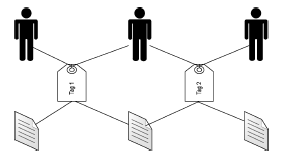
\includegraphics[width=0.75\textwidth]{gambar/skema automatic tag.PNG}
    \caption{Relasi antara user, tag, dan dokumen \citep{song2011autotag}}
    \label{gambar:relasi_user_tag_dokumen}
\end{figure}

Dengan relasi pada gambar \ref{gambar:relasi_user_tag_dokumen} , rekomendasi \textit{tag} dapat dilakukan dengan dua jenis menurut Song yaitu jenis pendekatan melalui pengguna dan jenis pendekatan melalui dokumen. Rekomendasi \textit{tag} merupakan suatu sistem yang di mana sistem tersebut menampilkan \textit{tag} yang relevan pada suatu dokumen agar pengguna bisa memperhitungkan apakah \textit{tag} yang ditampilkan itu ingin dipakai atau tidak. Melalui pendekatan \textit{user}, sistem ini akan mengolah rekomendasi \textit{tag} berdasarkan \textit{tag-tag} yang telah dilakukan \textit{user} sebelumnya dan merekomendasikan tag yang mirip dengan \textit{user} ini atau kelompok dari \textit{user} tersebut. Berbeda halnya dengan pendekatan dokumen, cara ini dilakukan dengan cara mengklasterisasikan dokumen-dokumen tersebut ke dalam topik-topik yang berbeda. Topik yang sama pada suatu dokumen akan memiliki \textit{tag} yang diasumsikan lebih mirip dibandingkan dokumen yang berbeda topik. Namun, di antara kedua cara ini, yang dinilai kurang efektif adalah melalui pendekatan \textit{user}. Pertama, berdasarkan penelitian dari \cite{farooq_social_bookmarking}, distribusi dari \textit{user} vs \textit{tag} mengikuti \textit{long tail power law distribution}. Itu artinya, hanya sebagian kecil porsi dari \textit{user} yang melakukan \textit{tag} dengan panjang atau meluas. Sebagai tambahan, penggunaan \textit{tag} yang berulang juga terbilang rendah, tetapi pertumbuhan perbendaharaan \textit{tag} terus berkembang. Dengan sedikit pengguna relatif yang didapat, pendekatan \textit{user} akan sulit untuk mencari model mana yang cocok buat untuk melakukan rekomendasi \textit{tag} yang efektif. Berbanding terbalik dengan pendekatan dokumen yang lebih kokoh karena kekayaan informasi yang ada di dokumen. Bahkan, \textit{tag} dan kata akan menciptakan relasi yang potensial antara topik dan konten di suatu dokumen yang di mana tag dianggap sebagai kelas label untuk dokumen dalam skenario \textit{supervised learning} atau kesimpulan dari dokumen dalam skenario \textit{unsupervised learning}. \citep{song2011autotag}

Namun, percobaan ini hanya terbatas pada CiteULike dan del.icio.us. Untuk saat ini, kedua situs tersebut sudah tidak dapat diakses dengan semestinya. CiteULike beralih menjadi situs judi, sedangkan del.icio.us tidak dapat diakses oleh umum.
	
Beberapa tahun kemudian, suatu penelitian membahas mengenai \textit{automatic mashup tag}. Secara sederhana, \textit{mashup} adalah suatu \textit{web service} yang di mana merupakan kumpulan dari kombinasi beberapa Web \textit{API} dan konten dari berbagai sumber. Berbeda dengan rekomendasi \textit{tag} yang menggunakan pendekatan dengan konten tekstual, di dalam \textit{Web services} terdapat banyak sekali relasi seperti komposisi relasi antara \textit{mashup} dengan \textit{API} dan anotasi berelasi antara \textit{API} dan \textit{tag}. \citep{shi2016mashuptag}

\begin{figure}[H]
    \centering
    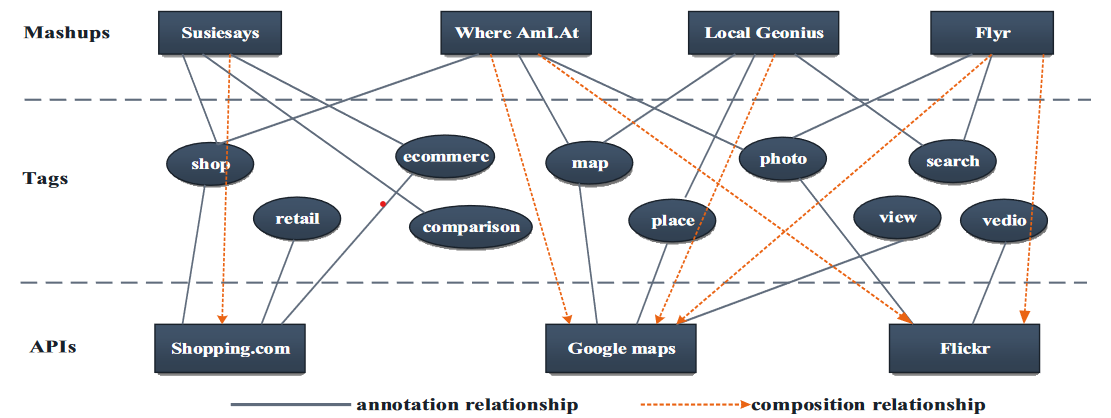
\includegraphics[width=1\textwidth]{gambar/mashup tag api.PNG}
    \caption{Skema \textit{Mashup}, \textit{Tag}, dan \textit{API} \citep{shi2016mashuptag}}
    \label{gambar:mashup_tag_api}
\end{figure}

Selain teks, \textit{tag} juga digunakan dalam hal yang bersifat non teks seperti video, musik, dan gambar. Dalam suatu video, \textit{tag} sangat diperlukan untuk menentukan relevansi antara pencarian yang diinginkan dengan isi video. Meskipun beberapa platform video seperti Youtube menyediakan judul dan deskripsinya, bisa saja judul tersebut tidak ada keterkaitannya dengan video dan deskripsinya yang sangat panjang sehingga orang malas untuk membaca. Manfaat dalam \textit{tag} video ada dua yaitu bisa menemukan daftar video yang representatif dan \textit{tag} dapat mendukung untuk melakukan penemuan tentang video yang kontennya berhubungan dengan video yang telah ditonton. \citep{parra2018videotag}

Untuk kasus \textit{automatic tag} pada musik, \textit{Automatic music tagging} adalah \textit{multi label binary classification} yang bertujuan untuk memprediksi \textit{tag} yang relevan pada suatu lagu. \textit{Tag} tersebut membawa informasi musik semantik yang nantinya dapat digunakan untuk membuat aplikasi seperti rekomendasi musik. \citep{won2020musictag}

Dengan demikian, peneliti ingin membuat penelitian terkait \textit{automatic tagging} dengan menggunakan penelitian dari \cite{song2008autotag} yang terdapat dua algoritma utama yaitu \textit{Bipartite Graph Partition} dan \textit{Two Way Poisson Mixture Model}.

\section{Rumusan Masalah}

Berdasarkan  latar belakang masalah yang telah diuraikan, maka perumusan masalah pada penelitian ini adalah "Bagaimana cara melakukan Automatic Tagging dengan menggunakan algoritma \textit{Bipartite Graph Partition} dan \textit{Two Way Poisson Mixture Model}?".

\section{Batasan Masalah}

Batasan masalah dalam penelitian ini yaitu:

\begin{enumerate}
    \item Data latih dan data uji yang digunakan berasal dari satu sumber \textit{web}.
    \item Untuk \textit{crawling} data, akan digunakan \textit{crawler} dari sistem yang telah dibuat oleh \cite{khatulistiwa_2022_searchengine} berjudul "Perancangan Arsitektur Search Engine dengan Mengintegrasikan Web Crawler, Algoritma Page Ranking, dan Document Ranking".
    \item Banyaknya $K$ yang digunakan adalah dua.
\end{enumerate}

\section{Tujuan Penelitian}

Tujuan dari penelitian ini adalah untuk membuat program \textit{automatic tagging} dengan menggunakan algoritma \textit{Bipartite Graph Partition} dan \textit{Two Way Poisson Mixture Model} sesuai penelitian \cite{song2008autotag}.

\section{Manfaat Penelitian}

Dalam penelitian ini, manfaat yang bisa diperoleh yaitu:

\begin{enumerate}
    \item Bagi Peneliti
    \begin{itemize}
        \item[] Menambah pengetahuan penulis tentang \textit{automatic tagging} terhadap dokumen.
    \end{itemize}
    \item Bagi Peneliti Selanjutnya
    \begin{itemize}
        \item[] Diharapkan metode yang diusulkan pada penelitian ini dapat membantu penelitian selanjutnya dalam mengembangkan sistem yang lebih kompleks dan bermanfaat.
    \end{itemize}
\end{enumerate}


% Baris ini digunakan untuk membantu dalam melakukan sitasi
% Karena diapit dengan comment, maka baris ini akan diabaikan
% oleh compiler LaTeX.
\begin{comment}
\bibliography{daftar-pustaka}
\end{comment}

 %!TEX root = ./template-skripsi.tex
%-------------------------------------------------------------------------------
%                            BAB II
%               KAJIAN TEORI
%-------------------------------------------------------------------------------

\chapter{KAJIAN PUSTAKA} 

% \section{Related Work}

% \textit{\textbf{Bipartite Graph Partitioning}}: sebuah \textit{bipartite graph} yang terdiri dari dua set \textit{disjoint} dari titik-titik X dan Y yang tidak ada garis yang memiliki masing-masing \textit{end point} di dalam set yang sama. Masalah \textit{graph partitioning} secara umum adalah \textit{NP hard} untuk \textit{bipartite graph}, \textit{partitioning} teroptimasi dengan meminimalisir suatu \textit{global function}. Banyak algoritma klastering yang telah diajukan untuk melakukan \textit{partitioning} pada \textit{bipartite graph}. Algoritma \textit{Min-Max Cut} meminimalisir total bobot di antara klaster dan memaksimalkan total bobot di dalam klaster. \textit{Spectral Clustering} secara bersamaan mengklasterkan baris dan kolom dari \textit{adjacency matrix} dari suatu graf. Namun, \textit{spectral clustering} bisa gagal dalam beberapa kasus di mana dua \textit{bipartite graph} bersatu menjadi suatu \textit{tripartite graph} karena sifat keheterogenan dari titik-titik. Untuk mengatasinya, algoritm \textit{Consistent Bipartite Graph Co-partitioning (CBGC)} diajukan. \textit{CBGC} mengaplikasikan \textit{semi-definite programming (SDP)} untuk mengatasi \textit{star-structured high order heterogeneous data} dengan merepresentasikan mereka sebagai beberapa graf \textit{bipartite} dan mengoptimalkan \textit{global function} untuk mencari pemotongan terbaik. Namun, CBGC hanya bisa mengatasi \textit{binary clustering problem} dan tidak cocok untuk pekerjaan multiklastering.

% \textit{\textbf{Low Rank Matrix Approximation}}: \textit{Low rank matrix approximation} adalah suatu permasalahan terkait aproksimasi \(m x n\) matriks \(A\) dengan matriks rank \(k\) yang lain, di mana \(k\) lebih kecil dibandingkan \(m\) dan \(n\). Metode tradisional seperti \textit{Singular Value Decomposition (SVD)} bisa digunakan untuk mencari matriks tersebut, tetapi waktu komputasinya biasanya sangat lama yaitu \(Omin\{mn^2, nm^2\}\).

% Sebelumnya, metode \textit{near-optimal} \textit{low rank matrix approximation} mulai menjadi populer. Jika kita \textit{denote} \(A_k\) sebagai aproksimasi optimal rank \(k\) dari matriks \(A\), tujuannya adalah untuk mencari \textit{near-optimal} matriks \(A_k^*\) yang meminimalisir error \(e\):

% \begin{equation}
%     ||A - A_k^*|| \leq ||A - A_k|| + e
% \end{equation}

% Dekomposisi \(CUR\) merupakan salah satu algoritma yang aproksimasi \(A\) dengan \(A = CUR\), di mana \(C\) adalah matriks \textit{consisting} dari angka-angka kecil dari kolom \(A\), \(R\) adalah matriks \textit{consisting} dari angka-angka kecil di baris \(A\), dan \(U\) adalah matriks \textit{appropriately defined low dimensional encoding}. Dengan demikian, \(CUR\) matriks dekomposisi menyediakan \textit{dimensionally reduced low rank approximation} menjadi data matriks orisinil \(A\) yang terdiri dari angka kecil dari kolom sekarang dan baris dari matriks original. Secara waktu baik linear dan konstan dari algoritma \(CUR\) telah diusulkan menjadi mengaproksimasikan matriks berukuran besar secara efisien.Namun, sejak baris dan kolom dipilih secara random, \(CUR\) tidak bisa memastikan akan matriks yang simetris. Hal ini membuatnya tidak cocok untuk kasus \textit{bipartite graph} karena \textit{biparite graph} membutuhkan beban matriks yang selalu simetris.

\section{Representasi Bipartite Graph}

Mendefinisikan suatu graf \(G = (V, E, W)\) sebagai suatu set dari titik-titik \(V\) dan hubungan mereka dengan garis \(E\), dengan \(W\) sebagai bobot dari garis-garis tersebut. Sebagai contoh, \(w_{ij}\) sebagai bobot dari garis di antara titik \(i\) dan \(j\).

Graf $G$ disebut \textit{bipartite} jika mengandung dua kelas titik $X$ dan $Y$ sebagai berikut $V = X \cup Y$ dan $X \cap Y = \emptyset$ setiap garis $e_{ij} \in E$ memiliki \textit{endpoint} $i$ di dalam $X$ dan \textit{endpoint} lain $j$ di dalam $Y$. Biasanya, $X$ dan $Y$ merujuk kepada perbedaan tipe objek dan $E$ merepresentasikan relasi antara keduanya. Di dalam konteks representasi dokumen, $X$ merupakan suatu set dokumen, sedangkan $Y$ adalah \textit{terms} dan $w_{ij}$ merupakan banyaknya \textit{term} $j$ yang muncul di dalam dokumen $i$. Perlu dicatat bahwa \textit{weighted adjacency matrix} $W$ untuk \textit{bipartite graph} selalu simetris. Sebagai contoh, gambar berikut adalah \textit{undirected bipartite graph} dengan 4 dokumen dan 5 \textit{term}.

\begin{figure}[h]
    \centering
    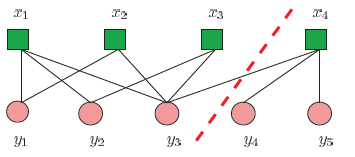
\includegraphics[width=0.75\textwidth]{gambar/Bipartite Graph.PNG}
    \caption{Suatu \textit{bipartite graph} \(X\) dan \(Y\) \cite{song2008autotag}}
    \label{gambar:bipartite_graph}
\end{figure}

\subsection{Normalisasi dan Aproksimasi}

Normalisasi biasanya digunakan pertama kali untuk bobot matriks \(W\) untuk mengeliminasi \textit{bias}. Jalur yang paling lurus untuk menormalisasikan \(W\) adalah normalisasi baris yang tidak mengambil akun dari simetri pada \(W\). Namun, untuk memahami simetri pada \(W\), Song dkk menggunakan \textit{normalized graph Laplacian} untuk aproksimasi \(W\). \textit{Normalized Laplacian} \(L(W)\) sebagai berikut.

\begin{align*}
L(W)_{i j} = \begin{cases}1-\frac{w_{i j}}{d_{i}} & \text { jika } i=j, \\ -\frac{w_{i j}}{\sqrt{d_{i} d_{j}}} & \text { jika } i \text { dan } j \text { terhubung } \\ 0 & \text { selain itu, }\end{cases}
\end{align*}

di mana \(d_i\) adalah \textit{degree} luar dari titik \(i\), pada persamaan $d_{i}=\sum w_{i j}, \forall j \in$ $V$. Kemudian, kita bisa mendefinisikan matriks diagonal \(D\) di mana $D_{ii} = d_i$. Oleh karena itu, \textit{normalize Laplacian} dapat direpresentasikan sebagai berikut. 

\begin{equation}
\label{normalize_laplacian}
    L(W) = D^{(-1/2)}WD^{(-1/2)}
\end{equation}

Untuk \textit{dataset} berskala besar seperti situs \textit{corpora} dan koleksi gambar, spasi fitur mereka biasanya mengandung jutaan vektor dengan dimensi yang sangat tinggi (contohnya, \(x\) = $10^6$, y = $10^7$). Oleh karena itu, biasanya ini sering diinginkan untuk mencari \textit{low rank matrix $W$ komplemen} untuk aproksimasi $L(W)$ dengan tujuan untuk mengurangi biaya komputasi, mengekstrak korelasi, dan menghapus \textit{noise}. Metode dekomposisi matriks tradisional misalnya adalah \textit{Single Value Decomposition} dan \textit{eigenvalue decomposition}, membutuhkan waktu \textit{superlienar} untuk perkalian matriks vektor jadi biasanya mereka tidak menggunakannya sampai pengaplikasian di dunia nyata.

Untuk \textit{symmetric low rank apporiximation}, di sini menggunakan algoritma Lanczos yang secara iteratif mencari nilai eigen dan vektor eigen dari matriks persegi. Diberikan $n$ x $n$ \textit{sparse symmetric matrix} $A$ dengan nilai eigen:

\begin{equation}
\label{lambda_lambda}
    \lambda \geq ... \geq \lambda_n \geq 0
\end{equation}

Algoritma Lanczos menghitung $k$ x $k$ \textit{symmetric tridiagonal matrix} $T$, yang nilai eigennya mengaproksimasi nilai eigen dari $A$, dan vektor eigen dari $T$ bisa digunakan untuk mengaproksimasi vektor eigen $A$, dengan $k$ lebih kecil dibandingkan $n$. Dengan kata lain, $T$ yaitu:

\begin{equation}
\label{frobenius_norm}
    ||A - T||_F \leq e||A||_F
\end{equation}

di mana $||.||_F$ denotasi \textit{Frobenius norm}, dengan \(e\) sebagai variabel terkendali. Sebagai contoh, untuk menangkap \(95 \% \) varians dari \(A\), \(e\) diatur sebagai 0.05.

\subsection{Bipartite Graph Partitioning}

Untuk melakukan multi-klastering pada \textit{bipartite graph}, \cite{song2008autotag} menggunakan algoritma \textit{Spectral Recursive Embedding (SRE)}. Secara esensial, \textit{SRE} digunakan untuk menkontruksi \textit{partition} dengan meminimalisir normalisasi dari total pada bobot garis di antara pasangan yang tidak cocok pada suatu garis, misalnya \(min_{\Pi(A,B)}Ncut(A,B)\), di mana \(A\) dan \(B\) adalah pasangan yang cocok dalam partisi dengan $A^c$ dan $B^c$ menjadi yang lain. Normalisasi varian dari \textit{edge cut} \(Ncut(A,B)\) didefinisikan sebagai berikut.

\begin{equation}
    \label{n_cut}
    Ncut(A,B) = \frac{cut(A,B)}{W(A,Y)+W(X,B)} + \frac{cut(A^c,B^c)}{W(A^c,Y)+W(X,B^c)},
\end{equation}

di mana

\begin{equation}
\begin{split}
\label{cut_ab}
    cut(A,B) &= W(A,B^c) + W(A^c, B) \\
             &= \sum_{i \in A, j \in B^c}{} w_{ij} + \sum_{i \in A^c, j \in B}{} w_{ij},
\end{split}
\end{equation}

Rasional dari \(Ncut\) tidak hanya mencari partisi dengan perpotongan garis kecil, tetapi juga mepartisinya sepadat mungkin. Ini berguna untuk aplikasi dari \textit{tagging document} di mana dokumen dengan setiap partisi secara ideal berfokus kepada satu topik spesifik. Sebagai hasil, semakin padat suatu partisi, semakin baik yang dokumen relevan dan \textit{tag} terkelompokkan bersamaan.

\subsection{Dengan Cluster Node Ranking}

\cite{song2008autotag} mendefinisikan dua pengukuran baru \textit{N-Precision} dan \textit{N-Recall} untuk \textit{node ranking}. \textit{N-Precision} dari titik \(i\) merupakan jumlah total dari bobot pada garis yang terkoneksi kepada titik dalam klaster yang sama, dibagi dengan jumlah total dari bobot garis yang ada di dalam klaster. Label klaster \(i\) sebagai \(C(i)\),

\begin{equation}
\label{n_precision}
    np_i=\frac{\sum_{j=1}^{n}w_{ij}\Pi[C(j) = C(i)]}{\sum_{j,k=1}^{n}w_{jk}\Pi[C(j) = C(k) = C(i)]},j,k\neq i,
\end{equation}

Untuk graf tidak berbobot, persamaan di atas setara dengan banyaknya garis yang berasosiasi dengan titik \(i\) di dalam klaster \(C(i)\), dibagi dengan total garis yang ada di dalam klaster \(C(i)\). Secara umum, \textit{N-precision} mengukur seberapa pentingnya titik pada suatu klaster, di dalam perbandingan dengan titik lain. Dalam konteks pada suatu dokumen, klasternya adalah suatu set topik dari dokumen dan bobot dari titik-titik kata menunjukkan frekuensi dari kata-kata yang muncul pada topik tersebut. Dengan \textit{cluster determined}, \textit{denominator equation} bersifat konstan, jadinya semakin banyak bobot yang dimiliki pada suatu titik, semakin penting pula.

Kontrasnya, \textit{N-recall} digunakan untuk menghitungkan probabilitas posterior dari titik \(i\) pada klaster yang diberikan dan \textit{inverse} pembagian dari garis i yang berasosiasi dengan klasternya.

\begin{equation} \label{n_recall}
    nr_i= \frac{|E_i|}{\sum_{j=1}^{n}w_{ij}\Pi[C(j) = C(i)]}.
\end{equation}

Hal tersebut merupakan bukti bahwa \textit{N-Recall} selalu tidak kurang dari satu. Semakin lebar \textit{N-Recall}, maka semakin mungkin bahwa kata tersebut berasosiasi dengan suatu topik yang spesifik.

Diberikan \(np_i\) dan \(nr_i\), kita akan melakukan estimasi dari peringkat \(i\):

\begin{equation}\label{rank_i}
\begin{split}
    Rank_i = \begin{cases} \exp(-\frac{1}{r(i)^2}) , & r(i) \neq 0, \\
    0, & r(i) = 0, \\
    \end{cases}
    \textbf{di mana}\, r(i) = (np_i) * log(nr_i)
\end{split}
\end{equation}


Berdasarkan persamaan di atas, fungsi perangkingan dari \cite{song2008autotag} merupakan pengganti yang dihaluskan yang proporsional untuk presisi titik (\textit{node precision}) dan \textit{recall}, hasilnya terjamin berada di kisaran \textit{range (0, 1)}.

Potensi pengalikasian dari metodologi \textit{bipartite graph node ranking} termasuk interpetasi relasi dokumen dan \textit{author} yaitu menentukan relasi sosial (misal "\textit{hub}" dan "\textit{authority}") dari \textit{author} di dalam satu topik penelitian yang sama, dan mencari representatif dokumen dari suatu topik. Di sini, mereka mengaplikasikan \textit{framework} ini untuk melakukan rekomendasi \textit{tag} dengan \textit{ranking node} yang merepresentasikan \textit{tag} pada setiap klaster.
\begin{figure}[H]
    \centering
    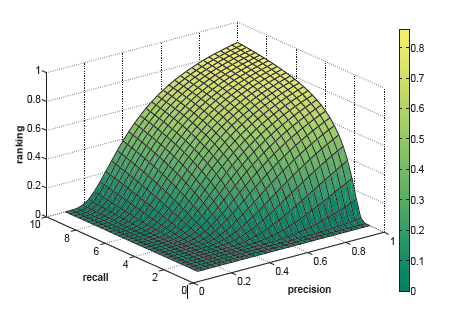
\includegraphics[width=0.75\textwidth]{gambar/Smoothed Ranking Function.PNG}
    \caption{Smoothed Ranking Function \cite{song2008autotag}}
    \label{gambar:smoothed_ranking_function}
\end{figure}

\section{Online Tag Recommendation}

Suatu dokumen biasanya mengandung beberapa kata dan beberapa \textit{tag} yang dibuat oleh \textit{user}. Hubungan antara dokumen, kata-kata, dan \textit{tag} bisa direpresentasikan dengan gambar dua \textit{bipartite graph} yang akan ditunjukkan oleh gambar setelah ini. 

Graf yang berbobot dapat ditulis dsebagai berikut
\begin{equation} \label{w_ab}
    W = \begin{pmatrix}
0 & A & 0\\
A^T & 0 & B\\
0 & B^T & 0
\end{pmatrix}
\end{equation}
di mana \(A\) dan \(B\) sebagai matriks-matriks inter-relasi antara \textit{tag} dengan dokumen dan dokumen dengan kata-kata.

\begin{figure}[H]
    \centering
    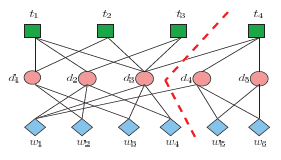
\includegraphics[width=0.75\textwidth]{gambar/Two Bipartite Graph of Tag Document Word.PNG}
    \caption{Dua bipartite graph dari dokumen-dokumen, kumpulan kata, dan kumpulan tag. \cite{song2008autotag}}
    \label{gambar:smoothed_ranking_function}
\end{figure}

Diberikan suatu representasi matriks, pendekatan lurus untuk \textit{tag} rekomendasi adalah dengan melihat kemiripannya antara dokumen \textit{query} dan dokumen \textit{training} dengan fitur-fitur kata, kemudian lakukan \textit{top ranked tags} dari dokumen yang paling mirip. Pendekatan ini biasanya direferensikan sebagai filter kolaborasi. Namun, pendekatan ini tidaklah efisien untuk skenario dunia nyata. Untuk mengambil kelebihan dari algoritma \textit{node ranking}, Song dkk menggunakan \textit{Possion Mixture Model (PMM)} yang secara efisien menentukan sampel \textit{membership} sebaik klastering kata-kata dengan makna yang mirip. Sebelum melakukan  \textit{mixture model}, di sini terdapat rangkuman algoritma yang digunakan untuk rekomendasi \textit{tag} di dalam Algoritma 1. (\cite{song2008autotag})

\begin{algorithm} [H]
\caption{Online Tag Recommendation \citep*{song2008autotag}}\label{alg:online_tag_recommendation}
\begin{algorithmic}
\State 1: \textbf{Input} $(\mathcal{D}, S, T), K, M, L$ \\
$\quad$ Kumpulan dokumen: $\mathcal{D}=\left\{\mathcal{D}_{1}, \ldots, \mathcal{D}_{m}\right\}$ \\
$\quad$ \textit{Word vocabulary}: $S=\left\{S_{1}, \ldots, S_{k}\right\}$ \\
$\quad$ \textit{Tag vocabulary}: $T=\left\{T_{1}, \ldots, T_{n}\right\}$ \\
$\quad$ banyaknya klaster: $K \in \mathbb{R}$ \\
$\quad$ banyaknya komponen-komponen: $M \in \mathbb{R}$ \\
$\quad$ banyaknya klaster-klaster kata: $ L \in \mathbb{R} $ \\
\textit{\textbf{Offline Computation}} \\
2: Menunjukkan bobot terdekat matriks W seperti persamaan (\ref{w_ab}) \\
3: Normalisasi $W$ menggunakan \textit{Normalized Laplacian} persamaan (\ref{normalize_laplacian}) \\
4: Komputasi \textit{low rank approximation matrix} menggunakan Lanczos: \\
$\quad \tilde{W} \simeq L(W)=Q_{k} T_{k} Q_{k}^{T}$ \\
5: Partisi $\tilde{W}$ ke dalam klaster K menggunakan SRE, 
$\quad \tilde{W}=\left\{\tilde{W}_{1}, \ldots, \tilde{W}_{K}\right\}$ \\
6: Tandai label ke dalam setiap dokumen $\mathcal{D}_{j}, j \in\{1, \ldots m\}$ \\
$\quad C\left(\mathcal{D}_{j}\right) \in\{1, \ldots, K\}$ \\
7: Hitung \textit{node rank} $Rank(T)$ untuk setiap tag $T_{i, k}$ di dalam klaster \\
$k, i \in\{1, \ldots, n\}, k\{1, \ldots, K\} \quad$ persamaan (\ref{rank_i}) \\
8: Buat \textit{Poisson Mixture Model} untuk $(\tilde{B}, C(\mathcal{D}))$ dengan $M$ komponen-komponen dan $L$ klaster kata-kata, di mana $\tilde{B}$ denotasi matriks inter-relationship pada suatu dokumen-dokumen dan kata-kata di dalam $\tilde{W}$ persamaan (\ref{w_ab})\\
\textit{\textbf{Online Recommendation}} \\
9: Untuk setiap dokumen tes $\mathbb{Y}$, kalkulasikan posterior probabilitas \\
$P(C=k \mid D=\mathbb{Y})$ di dalam setiap klaster $k$, dan denotasi membership pada $\mathbb{Y}$ sebagai $C(\mathbb{Y})=\{c(\mathbb{Y}, 1), \ldots, c(\mathbb{Y}, K)\}$ persamaan (\ref{bayes_rules}) \\
10: Tag rekomendasi berdasarkan perangkingan pada tag, yaitu \textit{joint probability} pada tag-tag $T$ dan dokumen $Y$, $R(T, \mathbb{Y})$ persamaan (\ref{rank_tag}) \\
\end{algorithmic}
\end{algorithm}

Dua tahap \textit{framework} ini bisa diinterpretasikan sebagai prosedur \textit{unsupervised-supervised learning}. Saat tahap \textit{offline learning stage}, titik-titik akan dipartisi ke dalam klaster-klaster menggunakan \textit{unsupervised learning}, label klaster dipasangkan kepada \textit{document node} sebagai \textit{class label} mereka, dan tag akan diberikan \textit{rank} di dalam setiap klaster. \textit{Mixture model} kemudian dibangun berdasarkan distribusi dari dokumen-dokumen dan kata-kata. Di dalam \textit{online recommendation stage}, suatu dokumen diklasifikasikan ke dalam \textit{predefined cluster} yang telah didapatkan di dalam tahap pertama oleh Naive Bayes jadi \textit{tag} tersebut bisa direkomendasikan di pengurutan secara terbalik dari rank mereka. Untuk menghindari kebingungan, \cite{song2008autotag} akan merujuk kepada klaster yang diinginkan dengan mempartisi algoritima di dalam tahap pertama sebagai \textit{classess} di dalam sesi selanjutnya. (\cite{song2008autotag})

\subsection{Two-Way Poisson Mixture Model}

\cite{song2008autotag} mengusulkan untuk menggunakan \textit{Poisson Mixture Model} untuk mengestimasi distribusi data pada vektor dokumen sebab algoritma tersebut  cocok digunakan dibandingkan \textit{standard Poissons} dengan memproduksi estimasi lebih baik pada data varians dan cukup mudah untuk estimasi parameter. Akan tetapi, itu membutuhkan waktu untuk mencocokkan data latihan. Algoritma ini efisien untuk memprediksi label kelas dari dokumen baru setelah model tersebut selesai dibuat. Karena stabilitas numerikal pada pendekatan statistika ini, biasanya hasilnya dapat diandalkan. Sejak hanya estimasi probabilitas yang dilibatkan, ini dapat diandalkan untuk proses secara \textit{real-time}.

Namun, pendekatan tradisional \textit{unsupervised learning} dari \textit{mixture model} tidak selalu diandalkan untuk menghadapi klasifikasi dokumen. Mempertimbangkan kelemahan dan tingginya dimensi pada matriks \textit{document-word} di mana kebanyakan masukkan berupa 0 dan 1, model bisa saja gagal untuk memprediksi distribusi yang benar (yaitu \textit{probability mass faunction}) pada komponen yang berbeda. Sebagai hasilnya, klasterisasi kata adalah langkah yang diperlukan sebelum mengestimasi komponen-komponen di dalam model. Di sini akan dilakukan \textit{two-way Poisson Mixture Model} untuk secara bersamaan melakukan \textit{cluster word feature} dan klasifikasi dokumen.

\begin{figure}[H]
    \centering
    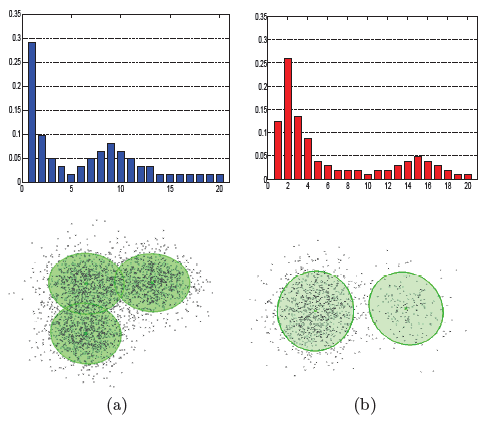
\includegraphics[width=0.75\textwidth]{gambar/Poisson Distribution in Two Cluster.PNG}
    \caption{Distribusi Poisson dalam dua klaster. Bagian atas menggambarkan histogram dari \textit{mixture components}. Bagian bawah menggambarkan hasil dari klasifikasi \textit{mixture model}. Bagian (a) \textit{three component mixtures} dan bagian (b) \textit{two component mixtures} \cite{song2008autotag}}
    \label{gambar:distribution_poisson}
\end{figure}

Diberikan suatu dokumen \(D = \{D_1, ..., D_p\}\), di mana \(p\) adalah dimensi, distribusi pada vektor dokumen di setiap kelas dapat diestimasikan dengan menggunakan \textit{parametric mixture model}.

kelas label \(C = \{1,2,...,K\},\) kemudian
\begin{equation}
\label{poisson_mixture_model_1}
    P(D = d | C = k) = \sum_{m=1}^{M}\pi_m\Pi(F(m) = k) \prod_{j=1}^{p}\phi(d_j|\lambda_{j,m}),
\end{equation}

di mana \(\pi_m\) adalah \textit{prior probability} dari komponen \(m\), dengan \(\sum_{m=1}^{M}\pi_m = 1\).\(\Pi(F(m) = k)\) adalah fungsi indikator yaitu apakah komponen \(m\) milik kelas \(k\), dan \(\phi\) merujuk kepada \textit{probability mass function} dari distribusi Poisson, \(\phi(d_j|\lambda_{j,m}) = e^{-\lambda_{j,m}}\lambda_{j,m^{d_j}}/ d_j\)!.

Pada jalur ini, setiap kelas adalah \textit{mixture model} dengan distribusi yang multivariasi dengan memiliki variabel yang mengikuti distribusi Poisson. Gambar 2.4 menunjukkan histogram pada dua \textit{mixture} yang bisa dianggap sebagai pmf dari dua \textit{Poisson mixture}.

Asumsi \cite{song2008autotag} terkait setiap kelas, kata-kata pada dokumen yang berbeda memiliki parameter Poisson yang setara, saat dokumen-dokumen di dalam kelas yang berbeda, kata-kata bisa saja mengikuti perbedaan distribusi Poissson. Untuk mempersimpel, \cite{song2008autotag} mengasumsi bahwa semua kelas memiliki nomor yang dari klaster-klaster kata. \textit{Denote} \(l = \{1,,,,L\}\) untuk menjadi klaster-klaster kata, kata-kata yang sama klaster kata \(m\) akan memiliki parameter yang sama yaitu \(\lambda_{i,m} = \lambda_{j,m} = \lambda_{l,m}\) untuk \(c(i,k) = c(j,k)\) di mana \(c(i,k)\) \textit{denote} label klaster pada kata \(i\) di dalam kelas \(k\). Berarti, persamaan sebelumnya dapat dipermudah menjadi (dengan $L \ll p$):

\begin{equation}
\label{poisson_mixture_model_2}
    P(D = d | C = k) \propto \sum_{m=1}^{M}\pi_m\Pi(F(m) = k) \prod_{l=1}^{L}\phi(d_{k,l}|\lambda_{l,m}),
\end{equation}

\subsubsection{Estimasi Parameter}

Dengan kelas yang dideterminasi, berikutnya masukkan algoritma EM untuk mengestimasi parameter Poisson \(\lambda_{l,m}, l \in \{1, ..., L\}, m \in \{1, ..., M\}\), \textit{prior of mixture component} \(\pi_m\), dan indeks klaster kata \(c(k,j) \in \{1, ..., L\},k \in \{1, ..., K\}, j \in \{1, ..., p\}\).

Estimasi \textit{E-step} \textit{posterior probability} \(p_{i,m}\) sebagai berikut.

\begin{equation}
\label{e_step}
p_{i, m} \propto \pi_{m}^{(t)} \mathbb{II}(C(i)) \prod_{j=1}^{p} \theta\left(d(i, j) \mid \tilde{\lambda}_{m, i, j}^{(t)}\right) 
\end{equation}

\textit{M-step} menggunakan \(p_{i,m}\) untuk memaksimalkan \textit{objective function}


\begin{equation}
\label{m_step}
\begin{aligned}
&\quad L\left(\pi_{m}^{(t+1)}, \tilde{\lambda}_{m, l}^{(t+1)}, c^{(t+1)}(k, j) \mid \pi_{m}^{(t)}, \tilde{\lambda}_{m, l}^{(t)}, c^{(t)}(k, j)\right) \\
&=\max \sum_{i=1}^{n} \sum_{m=1}^{M} p_{i, m} \log \left(\pi_{m}^{(t+1)} \mathbb{I}(C(i)) \prod_{j=1}^{p} \theta\left(d(i, j) \mid \tilde{\lambda}_{m, i, j}^{(t+1)}\right)\right),
\end{aligned}
\end{equation}


dan \textit{update} parameter


\begin{equation}
\label{update_parameter_pi}
\pi_{m}^{(t+1)}=\frac{\sum_{i=1}^{n} p_{i, m}}{\sum_{m^{\prime}=1}^{M} \sum_{i=1}^{n} p_{i, m^{\prime}}}, \\ \\ 
\end{equation}
\begin{equation}
\label{update_parameter_lambda}
\tilde{\lambda}_{m}^{(t+1)}=\frac{\sum_{i=1}^{n} p_{i, m} \sum_{j} d(i, j) \mathbb{I}(C(i))}{|d(i, j)| \sum_{i=1}^{n} p_{i, m}},
\end{equation}


di mana $|d(i,j)|$ denotasi bilangan dari $j$ di dalam komponen $l$.

Setelah $\tilde{\lambda}_{m}^{(t+1)}$ telah diperbaiki, indeks klaster kata $c^{(t+1)}(k, j)$ bisa ditemukan dengan melakukan \textit{linear search} pada semua komponen-komponen:

$$
c^{(t+1)}(k, j)=\arg \max _{l} \sum_{i=1}^{n} \sum_{m=1}^{M} \log \left(d(i, j) \mid \tilde{\lambda}_{m, l}^{(t+1)}\right)
$$

(\cite{song2008autotag})

\subsection{Tag Recommendation for New Documents}

Normalnya, label kelas $C(d_{t})$ dari suatu dokumen baru $d_t$ ditentukan oleh $\hat{C}(x)=\arg \max _{k} P\left(C=k \mid D=d_{t}\right)$. Namun, di kasus ini, \cite{song2008autotag} determinasi \textit{mixed membership} pada suatu dokumen dengan menkalkulasi \textit{posterior probabilities} pada suatu kelas dengan $\sum_{k=1}^{K} P\left(C=k \mid D=d_{t}\right)=1$. Mengaplikasikan persamaan (2.12) dan \textit{Bayes Rule},

\begin{equation}
\label{bayes_rules}
    \begin{split}
        P (C = k | D = d_t) 
        &= \frac{P(D = d_t | C = k) P(C=k)}{P(D=d_t)} \\
        &= \frac{\sum_{m=1}^{M} \pi_{m} \mathbb{II}(F(m)=k) \prod_{l=1}^{L} \phi(d_{k, l} \tilde{\lambda}_{l, m}) P(C=k)}{P(D=d_{t})}
    \end{split}
\end{equation}

di mana $P(C = k)$ adalah \textit{prior probabilites} dari kelas $k$ dan set seragam. Akhirnya, probabilitas untuk setiap \textit{tag} $T_{i}, i \in$ $\{1, \ldots, n\}$ diasosiakan dengan sampel adalah

\begin{equation}
\label{rank_tag}
    \begin{split}
        R(T_{i}, d_{t})
        &= P(T=T_{i}|D=d_{t}) \\
        &= Rank_{T_{i}} * P(C=x|D=d_{t})
    \end{split}
\end{equation}

Dengan perangkingan \textit{tag} dari terbesar ke terkecil pada probabilitas mereka, \textit{top ranked tags} dipilih untuk rekomendasi. (\cite{song2008autotag})

\section{Mixture Model}

Salah satu \textit{Mixture Model} yang  biasa dipakai yaitu \textit{Gaussian Mixture Model} (\textit{GMM}), \textit{GMM} adalah suatu \textit{parametric probability density function} yang merepresentasikan \textit{weighted sum} dari kepadatan komponen \textit{Gaussian}. Biasanya, \textit{GMM} digunakan sebagai \textit{parametric model} dari distribusi probabilitas pada pengukuran yang kontinu. Parameter \textit{GMM} diestimasi dari data latih menggunakan algoritma \textit{Expectation-Maximization} (\textit{EM}).

\textit{Gaussian Mixture Model} adalah \textit{weighted sum} dari \textit{M} kepadatan komponen \textit{Gaussian} dengan persamaan sebagai berikut.

\begin{equation}
    \label{eq:gaussian_mixture_model}
    p(x|\lambda) = \sum_{i=1}^{M} w_i g(x|\mu_i, \Sigma_i)
\end{equation}

Di mana x adalah $D$ \textit{dimensional continuous} vektor data, $w_i$, i = 1, ...,$M$ adalah bobot mikstur, dan $g(x|miu_i, \Sigma_i)$, $i$ = 1,...,$M$ adalah kepadatan komponen \textit{Gaussian}. Kepadatan komponen \textit{Gaussian} adalah sebagai berikut.

\begin{equation}
    \label{eq:component_gaussian_densities}
    g(x|\mu_i, \Sigma_i) = \frac{1}{(2\Phi)^{D/2}|\Sigma_i|^{1/2}}
    exp\{-\frac{(x-\mu_i)'\Sigma_i^{-1}(x-\mu_i)}{2}\}
\end{equation}

dengan $\mu_i$ sebagai \textit{mean vector} dan $\sigma_i$ sebagai matriks kovarian. \textit{Mixture Weights} memenuhi persamaan $\sum_{i=1}^{M}w_i = 1$.

Beberapa parameter tersebut dikumpulkan menjadi persamaan berikut.

\begin{equation}
    \label{eq:lambda_gaussian_mixture_model}
    \lambda = \{w_i, \mu_i, \sigma_i\} \\
    i = 1, ..., M
\end{equation}

Pada tahap selanjutnya adalah menghitung \textit{Maximum Likelihood Parameter}. Diberikan data latih berupa vektor-vektor dan konfigurasi \textit{GMM}. Dari sini akan dilakukan estimasi dari parameter \textit{GMM} $\lambda$. Metode paling populer dalam menentukan ini adalah estimasi \textit{Maximum Likelihood}.

Tujuan \textit{Maximum Likelihood} adalah mencari parameter model yang memaksimalkan \textit{likelihood} pada GMM dari data latih yang diberikan. Untuk setiap $T$ \textit{training vector} $X$ = $\{x_1,...,x_T\}$, \textit{GMM likelihood}, asumsikan antar vektor adalah independen, maka sebagai berikut.

\begin{equation}
    \label{eq:gmm_likelihood}
    p(X|\lambda) = \prod_{t=1}^{T} p(x_t|\lambda)
\end{equation}

Sayangnya, persamaan ini adalah fungsi tidak linear dari parameter $\lambda$ dan tidak mungkin untuk melakukan pemaksimalan secara langsung. Namun, parameter \textit{Maximum Likelihood} dapat diestimasikan dengan cara iteratif dengan menggunakan algoritma \textit{Expectation-maximization} (\textit{EM}).

Ide dasar dari algoritma \textit{EM} adalah memulai model awal $\lambda$ untuk mengistmasi model baru $\tilde{\lambda}$ lalu menjadi $p(X|\tilde{\lambda}) \geq p(X|\lambda)$. Model baru akan menjadi model awal untuk iterasi selanjutnya dan proses tersebut akan berlanjut sampai batas tertentu yang ditetapkan. Model awal biasanya \textit{derived} dengan menggunakan \textit{VQ estimation}. (\cite{reynolds_gaussian_mixture_model})

Dalam setiap iterasi \textit{EM}, formula reestimasi selanjutnya akan digunakan untuk meningkatkan nilai \textit{likelihood}.

\textit{Mixture Weights}
\begin{equation}
    \label{eq:gmm_em_mixture_weight}
    \tilde{w}_i = \frac{1}{T} \sum_{t=1}^{T}Pr(i|x_t, \lambda)
\end{equation}

\textit{Means}
\begin{equation}
    \label{eq:gmm_em_means}
    \tilde{\mu}_i = \frac{\sum_{t=1}^{T}Pr(i|x_t, \lambda) x_t}{\sum_{t=1}^{T}Pr(i|x_t, \lambda)} 
\end{equation}

\textit{Varians}
\begin{equation}
    \label{eq:gmm_em_varians}
    \tilde{\sigma}^2_i = \frac{\sum_{t=1}^{T}Pr(i|x_t, \lambda) x_t^2}{\sum_{t=1}^{T}Pr(i|x_t, \lambda)}  - \tilde{\mu_i^2}
\end{equation}

Kemudian \textit{posterior probability} untuk komponen $i$ sebagai berikut.

\begin{equation}
    \label{eq:gmm_em_posterior_probability}
    Pr(i|x_t, \lambda) = \frac{w_i g(x_t|\mu_i, \Sigma_i)}{\sum_{k=1}^{M}w_k g(x_t|\mu_i, \Sigma_i)}
\end{equation}

Perbedaan antara Distribusi Gaussian dengan Distribusi Poisson sebagai berikut.

\begin{figure}[H]
    \centering
    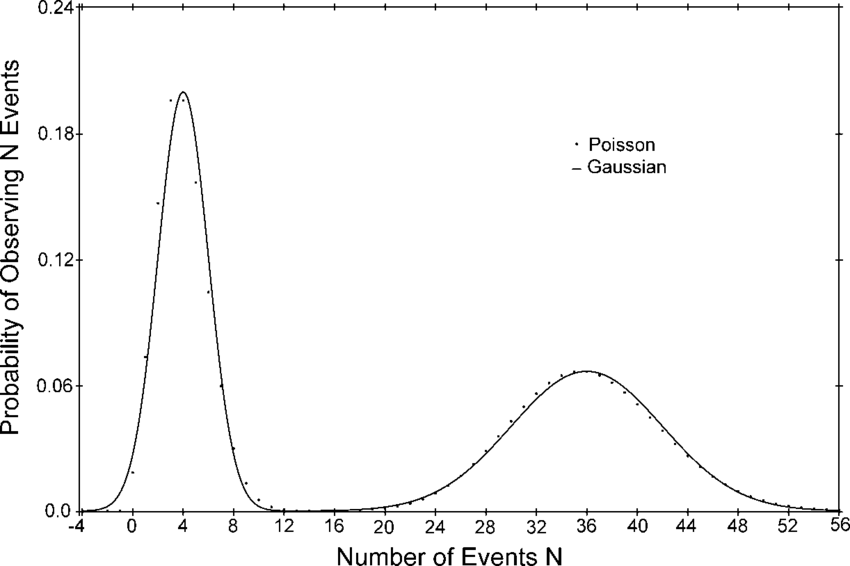
\includegraphics[width=0.50\textwidth]{gambar/Difference-between-Gaussian-and-Poisson-distributions-Graph-shows-two-Poisson-and-two.png}
    \caption{Perbedaan antara Distribusi Gaussian dengan Distribusi Poisson \cite{rzeszotarski_physics_tutorial}}
    \label{gambar:flowchart_automatic_tag}
\end{figure}

% \section{Lanczos Bidiagonalization dan SVD}

% Untuk mencari vektor singular baik kiri maupun kanan, diperlukan algoritma \textit{Lanczos Bidiagonalization}. Dalam algoritma tersebut terdapat, terdapat matriks penting seperti $U^T A V = B$ 

% \begin{align*}
%     U &= [u_1, ..., u_m] \\
%     V &= [v_1, ..., v_n] \\
%     U^TU &= I_m \\
%     V^TV &= I_n
% \end{align*}

% B adalah matriks \textit{bidiagonalization} sebagai berikut.

% \begin{equation*}
% B=\left[\begin{array}{ccccc}
% \alpha_{1} & \beta_{1} & & \ldots & 0 \\
% & \alpha_{2} & \beta_{2} & & \vdots \\
% &  & \alpha_{3} & \ddots & \\
% \vdots  & & & \ddots & \beta_{k-1} \\
% 0 & \ldots  & & & \alpha_{k}
% \end{array}\right] .
% \end{equation*}

% \begin{algorithm}[H]
% \caption{\textit{Lanczos Bidiagonalization Algorithm} \citep*{golub_matrix_computation_3_edition}}\label{alg:lanczos_bidiagonalization}
% \begin{algorithmic}
% \State $v_1 =$  given unit 2-norm n-vector ; $p_0 = v_1$
% % \State 
% \State $\beta_0 = 1$ ; $k = 0$ ; $u_0 = 0$
% % \State 
% \While{$\beta \neq 0$}
% \State $v_{k+1} = p_k/\beta_k$
% \State $k = k + 1$
% \State $r_k = Av_k - \beta_{k-1}u_{k-1}$
% \State $\alpha_k = \Vert r_k \|_2$
% \State $u_{k} = r_k/\alpha_k$
% \State $p_{k} = A^Tu_k-\alpha_kv_k$
% \State $\beta_k = \Vert p_k \|_2$
% \EndWhile
% \end{algorithmic}
% \end{algorithm}

% Dengan algoritma seperti itu, akan didapat hasil-hasil dari vektor singularnya.

%!TEX root = ./template-skripsi.tex
%-------------------------------------------------------------------------------
%                            BAB III
%               			PEMBAHASAN
%-------------------------------------------------------------------------------

\chapter{DESAIN MODEL}

\section{Tahapan Penelitian}

Berikut merupakan \emph{flowchart} dari tahapan penelitian \emph{Automatic Tagging} dengan menggunakan algoritma \emph{Bipartite Graph Partition} dan \emph{Two Way Poisson Mixture Model}.

\begin{figure}[H]
    \centering
    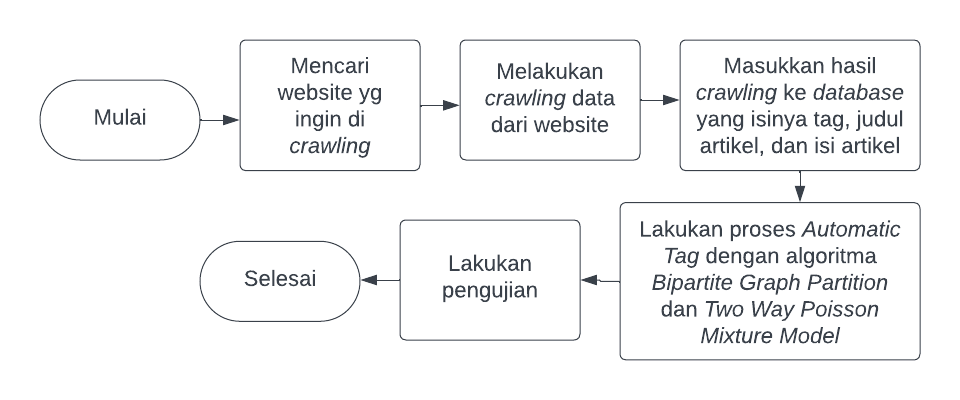
\includegraphics[width=1\textwidth]{gambar/Tahapan penelitian.png}
    \caption{Flowchart alur penelitian}
    \label{gambar:tahapan_penelitian}
\end{figure}

Mencari salah satu situs yang ingin di-\emph{crawling} terlebih dahulu. Kemudian, lakukan \emph{crawling} data dari situs tersebut menggunakan \emph{crawler} dari penelitian \cite{khatulistiwa_2022_searchengine}. Hasil \emph{crawling} tersebut dimasukkan ke dalam \emph{database}.

Kemudian, data tersebut diolah menggunakan algoritma \emph{Bipartite Graph Partition} dan \emph{Two Way Poisson Mixture Model} untuk melatih program supaya bisa memprediksi \emph{tag} yang diinginkan. Setelah itu, lakukan pengujian terhadap \emph{tag} yang telah dihasilkan.

% \section{Desain \textit{Automatic Tag }} 

% Pada proses pembuatan algoritma untuk pembuatan \textit{automatic tag}, penulis menggunakan algoritma \textit{Real Time Automatic Tag Recommendation}. 

% \textit{Real Time Automatic Tag Recommendation} berdasarkan algoritma yang dikembangkan oleh \citep{song2008autotag} adalah suatu sistem untuk merekomendasikan suatu \textit{tag-tag} untuk dokumen-dokumen yang di mana sistem ini memerlukan data latih. 

% Secara garis besar, algoritma ini memiliki dua tahap besar yaitu \textit{offline computation} atau tahap \textit{training data} dan \textit{online recommendation} atau tahap \textit{testing data}. 

% \textit{Offline computation} merupakan tahapan untuk mempelajari data-data dari kumpulan dokumen-dokumen ($D$), tag-tag ($T$), serta kata-kata ($S$) yang telah diberikan. Nantinya, data-data tersebut akan dibentuk ke dalam klaster-klaster ($K$) melalui algoritma \textit{Spectral Recursive Embedding} (\textit{SRE}). Selanjutnya, data-data yang telah diklaster, nantinya akan melakukan perangkingan terhadap suatu \textit{tag}. Selanjutnya, tahap untuk membuat \textit{Two Way Poisson Mixture Model}.

% Tahapan \textit{Online Recommendation} merupakan tahapan di mana suatu dokumen yang baru akan diberikan \textit{tag-tag} sesuai dengan klaster yang nantinya dokumen baru ini akan tempatkan.

% Tahapan \textit{Online Recommendation} merupakan tahapan di mana suatu dokumen yang baru saja diinput dan bukan yang diinput pada tahap \textit{Offline Computation} akan diberikan \textit{tag-tag} sesuai dengan klaster yang nantinya dokumen baru ini akan tempatkan.

\section{Algoritma \emph{Automatic Tag}}

Berikut adalah algoritma dari \textit{Online Tag Recommendation}

\begin{algorithm} [H]
\caption{Online Tag Recommendation \citep*{song2008autotag}}\label{alg:online_tag_recommendation_2}
\label{algoritma:automatic_tag}
\begin{algorithmic}
\State 1: \textbf{Input} $(\mathcal{D}, S, T), K, M, L$ \\
$\quad$ Kumpulan dokumen: $\mathcal{D}=\left\{\mathcal{D}_{1}, \ldots, \mathcal{D}_{m}\right\}$ \\
$\quad$ \textit{Word vocabulary}: $S=\left\{S_{1}, \ldots, S_{k}\right\}$ \\
$\quad$ \textit{Tag vocabulary}: $T=\left\{T_{1}, \ldots, T_{n}\right\}$ \\
$\quad$ banyaknya klaster: $K \in \mathbb{R}$ \\
$\quad$ banyaknya komponen-komponen: $M \in \mathbb{R}$ \\
$\quad$ banyaknya klaster-klaster kata: $ L \in \mathbb{R} $ \\
\textit{\textbf{Offline Computation}} \\
2: Menunjukkan bobot terdekat matriks W seperti persamaan (\ref{w_ab}) \\
3: Normalisasi $W$ menggunakan \textit{Normalized Laplacian} persamaan (\ref{normalize_laplacian}) \\
4: Komputasi \textit{low rank approximation matrix} menggunakan Lanczos: \\
$\quad \tilde{W} \simeq L(W)=Q_{k} T_{k} Q_{k}^{T}$ \\
5: Partisi $\tilde{W}$ ke dalam klaster K menggunakan SRE, 
$\quad \tilde{W}=\left\{\tilde{W}_{1}, \ldots, \tilde{W}_{K}\right\}$ \\
6: Tandai label ke dalam setiap dokumen $\mathcal{D}_{j}, j \in\{1, \ldots m\}$ \\
$\quad C\left(\mathcal{D}_{j}\right) \in\{1, \ldots, K\}$ \\
7: Hitung \textit{node rank} $Rank(T)$ untuk setiap tag $T_{i, k}$ di dalam klaster \\
$k, i \in\{1, \ldots, n\}, k\{1, \ldots, K\} \quad$ persamaan (\ref{rank_i}) \\
8: Buat \textit{Poisson Mixture Model} untuk $(\tilde{B}, C(\mathcal{D}))$ dengan $M$ komponen-komponen dan $L$ klaster kata-kata, di mana $\tilde{B}$ denotasi matriks inter-relationship pada suatu dokumen-dokumen dan kata-kata di dalam $\tilde{W}$ persamaan (\ref{w_ab})\\
\textit{\textbf{Online Recommendation}} \\
9: Untuk setiap dokumen tes $\mathbb{Y}$, kalkulasikan posterior probabilitas \\
$P(C=k \mid D=\mathbb{Y})$ di dalam setiap klaster $k$, dan denotasi membership pada $\mathbb{Y}$ sebagai $C(\mathbb{Y})=\{c(\mathbb{Y}, 1), \ldots, c(\mathbb{Y}, K)\}$ persamaan (\ref{bayes_rules}) \\
10: Tag rekomendasi berdasarkan perangkingan pada tag, yaitu \textit{joint probability} pada tag-tag $T$ dan dokumen $Y$, $R(T, \mathbb{Y})$ persamaan (\ref{rank_tag}) \\
\end{algorithmic}
\end{algorithm}

\section{Flowchart Automatic Tag}
\begin{figure}[H]
    \centering
    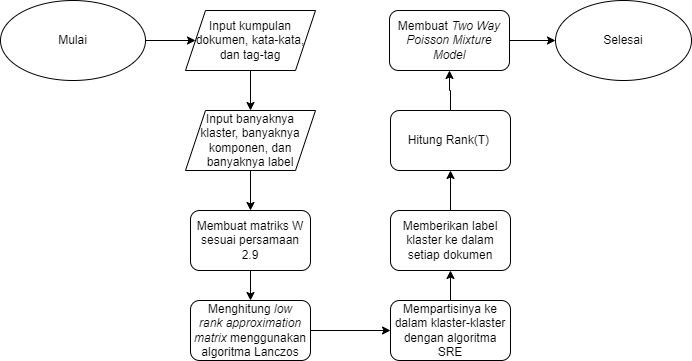
\includegraphics[width=1\textwidth]{gambar/Tag Flowchart.drawio.png}
    \caption{Diagram alir untuk tahap \textit{offline computation}}
    \label{gambar:flowchart_automatic_tag}
\end{figure}

\begin{figure}[H]
    \centering
    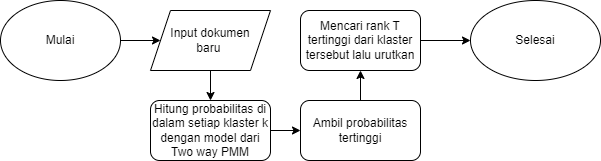
\includegraphics[width=1\textwidth]{gambar/Online Recommendation Flowchart.png}
    \caption{Melakukan \textit{online recommendation} berdasarkan hasil data training}
    \label{gambar:online_recomendation_tag}
\end{figure}

\section{Alat dan Bahan Penelitian}

Dalam penelitian ini, setidaknya ada perangkat keras sebagai berikut.

\begin{enumerate}
    \item Laptop dengan prosesor Intel Core i5 8th Gen \textit{series} dan \textit{RAM} 16 \textit{GB}.
    \item Koneksi berbasis Wi-Fi dan berbasis kuota internet dari ponsel pintar.
\end{enumerate}

Perangkat lunaknya sebagai berikut.

\begin{enumerate}
    \item Windows 10 64 bit OS.
    \item Visual Studio Code sebagai \textit{Code Editor}.
    \item Python 3 untuk menjalankan program Python.
    \item Sumber data berasal dari \textit{Thehill.com} .
\end{enumerate}

\section{Tahapan Penelitian Automatic Tag}

Setidaknya terdapat 10 tahapan yang perlu dijalankan agar \textit{automatic tag} ini akan berjalan dengan baik yaitu

\subsection{Penginputan}

Pada tahap ini, akan ditentukan enam komponen atau inputan yang diperlukan adalah dokumen ($D$), \textit{word vocabulary} ($S$), \textit{Tag vocabulary} ($T$), banyaknya klaster ($K$), banyaknya komponen-komponen ($M$), dan banyaknya klaster-klaster kata ($L$).

Untuk dokumen ($D$) yang diinput, berasal dari data hasil \textit{crawling} dengan menggunakan \textit{crawler} milik Lazuardy Khatulistiwa berjudul Perancangan Arsitektur \textit{Search Engine} dengan Mengintegrasikan \textit{Web Crawler}, Algoritma \textit{Page Ranking}, dan \textit{Document Ranking}.

Untuk \textit{word vocabulary} ($S$), kata-kata yang diinput merupakan kata-kata yang berasal dari dokumen hasil \textit{crawling}.

Pada \textit{tag vocabulary ($T$)}, \textit{tag} yang didapat berasal dari dokumen \textit{tag} hasil \textit{crawling}. 

Pada banyaknya klaster ($K$), digunakan untuk menentukan berapa klaster yang ingin dibuat saat menjalankan algoritma \textit{SRE}. Banyaknya klaster ini ditentukan sesuai dengan keinginan sang pengguna.

Banyaknya komponen-komponen ($M$), biasanya $M$ ini akan digunakan pada algoritma \textit{Two Way Poisson Mixture Model}.

Terakhir adalah banyaknya klaster kata ($L$) untuk melakukan pelabelan ($L$). Variabel ini akan digunakan pada algoritma \textit{Two Way Poisson Mixture Model}.

\subsection{Menentukan Matriks W}
Untuk matriks $W$ akan terdiri dari beragam matriks yaitu matriks $A$, matriks $A^T$, matriks $B$, dan matriks $B^T$.

Untuk matriks $A$, terbuat dari relasi antara \textit{tag vocabulary} dengan dokumen, sedangkan untuk matriks $B$ diperoleh dari relasi antara dokumen dengan \textit{word vocabulary}.

Untuk membuat matriks $W$ akan menggunakan persamaan (\ref{w_ab}). Untuk contohnya, akan mengambil gambar berikut.

\begin{figure}[h]
    \centering
    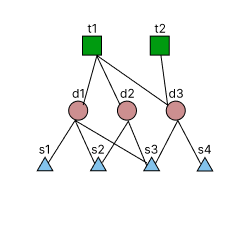
\includegraphics[width=0.75\textwidth]{gambar/Bipartite Graph Simple.png}
    \caption{Contoh simpel dua \textit{bipartite graph}}
    \label{gambar:simple_bipartite_graph}
\end{figure}

Relasi antara $t$ (\textit{tag}) dengan $d$ (\textit{document}) akan membentuk matriks $A$ dan $A^T$ sebagai berikut.

\begin{equation}
    A = \begin{pmatrix}
1 & 1 & 1 \\
0 & 0 & 1 \\
\end{pmatrix}
\end{equation}

\begin{equation}
    A^T = \begin{pmatrix}
1 & 0 \\
1 & 0 \\
1 & 1 \\
\end{pmatrix}
\end{equation}

Selanjutnya, mencari relasi antara $D$ (\textit{document}) dengan $S$ (\textit{words}) agar membentuk \textbf{matriks $B$} sebagai berikut.

\begin{equation}
    B = \begin{pmatrix}
1 & 1 & 1 & 0 \\
0 & 1 & 1 & 0 \\
0 & 0 & 1 & 1 \\
\end{pmatrix}
\end{equation}

\begin{equation}
    B^T = \begin{pmatrix}
1 & 0 & 0 \\
1 & 1 & 0 \\
1 & 1 & 1 \\
0 & 0 & 1 \\
\end{pmatrix}
\end{equation}

Selanjutnya, adanya penggabungan yang nantinya membentuk \textbf{matriks $W$} sebagai berikut

\begin{equation*}
    W = \begin{pmatrix}
0 & A & 0\\
A^T & 0 & B\\
0 & B^T & 0
\end{pmatrix}
\end{equation*}

Nantinya, matriks $A$ dan matriks $B$ ditempatkan ke dalam matriks $W$. Angka 0 di atas merupakan matriks 0 yang isinya menyesuaikan baris dan kolom matriks sekitarnya.

\begin{equation}
    W = \begin{pmatrix}
0 & 0 & 1 & 1 & 1 & 0 & 0 & 0 & 0 \\
0 & 0 & 0 & 0 & 1 & 0 & 0 & 0 & 0 \\
1 & 0 & 0 & 0 & 0 & 1 & 1 & 1 & 0 \\
1 & 0 & 0 & 0 & 0 & 0 & 1 & 1 & 0 \\
1 & 1 & 0 & 0 & 0 & 0 & 0 & 1 & 1 \\
0 & 0 & 1 & 0 & 0 & 0 & 0 & 0 & 0 \\
0 & 0 & 1 & 1 & 0 & 0 & 0 & 0 & 0 \\
0 & 0 & 1 & 1 & 1 & 0 & 0 & 0 & 0 \\
0 & 0 & 0 & 0 & 1 & 0 & 0 & 0 & 0 \\
\end{pmatrix}
\end{equation}

% \subsection{Normalisasi $W$ menggunakan \textit{Normalized Laplacian}}

% Pada persamaan normalisasi Laplacian, diperlukan dua jenis matriks yaitu matriks $W$ dan matriks $D$. Untuk mengisi matriks diagonal $D$ diperlukan mengisi $D_{ii}$ terlebih dahulu. Untuk mendapatkan $D_{ii}$ memerlukan $d_i$ yang berasal dari $d_{i}=\sum w_{i j}$ . $w_{ij}$ didapat dari matriks $W$.

% \begin{equation}
%     D = \begin{pmatrix}
% 3 & 0 & 0 & 0 & 0 & 0 & 0 & 0 & 0\\
% 0 & 1 & 0 & 0 & 0 & 0 & 0 & 0 & 0\\
% 0 & 0 & 4 & 0 & 0 & 0 & 0 & 0 & 0\\
% 0 & 0 & 0 & 3 & 0 & 0 & 0 & 0 & 0\\
% 0 & 0 & 0 & 0 & 4 & 0 & 0 & 0 & 0\\
% 0 & 0 & 0 & 0 & 0 & 1 & 0 & 0 & 0\\
% 0 & 0 & 0 & 0 & 0 & 0 & 2 & 0 & 0\\
% 0 & 0 & 0 & 0 & 0 & 0 & 0 & 3 & 0\\
% 0 & 0 & 0 & 0 & 0 & 0 & 0 & 0 & 1\\
% \end{pmatrix}
% \end{equation}

% Setelah mendapatkan $D$ dan $W$, lalu masukkan ke persamaan normalisasi Laplacian hingga membentuk $L(W)$. $L(W)$ yang dicontohkan di sini hasil dari pembulatan agar lebih mudah terbaca, tetapi dalam kasus nyatanya, tidak ada pembulatan.

% \begin{equation}
%     L(W) = \begin{pmatrix}
% 0 & 0 & 0.29 & 0.33 & 0.29 & 0 & 0 & 0 & 0\\
% 0 & 0 & 0 & 0 & 0.5 & 0 & 0 & 0 & 0\\
% 0.29 & 0 & 0 & 0 & 0 & 0.5 & 0.35 & 0.29 & 0\\
% 0.33 & 0 & 0 & 0 & 0 & 0 & 0.41 & 0.33 & 0\\
% 0.29 & 0.5 & 0 & 0 & 0 & 0 & 0 & 0.29 & 0.5 \\
% 0 & 0 & 0.5 & 0 & 0 & 0 & 0 & 0 & 0\\
% 0 & 0 & 0.35 & 0.41 & 0 & 0 & 0 & 0 & 0\\
% 0 & 0 & 0.29 & 0.33 & 0.29 & 0 & 0 & 0 & 0\\
% 0 & 0 & 0 & 0 & 0.5 & 0 & 0 & 0 & 0 \\
% \end{pmatrix}
% \end{equation}

\subsection{Menghitung \textit{Low Rank Approximation Matrix} menggunakan algoritma Lanczos}

Pada algoritma Lanczos yang terdapat di (\cite{golub_matrix_computation_3_edition}), ada beberapa inputan agar prosesnya bisa berjalan yaitu $\beta_0$, $q_0$, $b$, dan $q_1$. Berikut adalah beberapa inputannya.

\begin{equation*}
    \beta_0 = 0
\end{equation*}
\begin{equation*}
    q_0 = 0
\end{equation*}
\begin{equation*}
    b = arbitrary
\end{equation*}

Karena $b$ adalah \textit{arbitrary} yang memiliki makna bahwa nilai yang diinput itu bebas. Oleh karena itu, $b$ dibuat menjadi

\begin{equation*}
    b = \begin{pmatrix}
        1 & 1 & 1 & 1 & 1 & 1 & 1 & 1 & 1
    \end{pmatrix}
\end{equation*}

Selanjutnya nilai $q_1$ adalah

\begin{equation*}
    q_1 = b/||b|| = \begin{pmatrix}
        0.33 & 0.33 & 0.33 & 0.33 & 0.33 & 0.33 & 0.33 & 0.33 & 0.33 
    \end{pmatrix}
\end{equation*}

\begin{equation}
    \quad \hat{W} \simeq L(W)=Q_{k} T_{k} Q_{k}^{T}
\end{equation}

Karena persamaan ini, hasil dari $L(W)$ juga bisa dicari dengan menggunakan $\hat{W}$. Selain itu, algoritma Lanczos dinilai lebih efisien untuk data yang banyak dibandingkan menggunakan normalisasi Laplacian.  Untuk mencari $Q_k$ dan $T_k$, perlu menggunakan iterasi Lanczos. 

Untuk matriks $T_k$ memiliki format sebagai berikut

\begin{equation*}
T_{k}=\left[\begin{array}{ccccc}
\alpha_{1} & \beta_{1} & & & \\
\beta_{1} & \alpha_{2} & \beta_{2} & & \\
& \beta_{2} & \alpha_{3} & \ddots & \\
& & \ddots & \ddots & \beta_{k-1} \\
& & & \beta_{k-1} & \alpha_{k}
\end{array}\right] .
\end{equation*}

Dalam matriks di atas, diperlukan pencarian nilai $\alpha$ dan $\beta$ agar bisa melengkapi hasil $T_k$.

Untuk matriks $Q_k$ didapat dari
\begin{equation*}
    Q_k = \begin{pmatrix}
q_1 &|& q_2 &|& \dots &|& q_k
\end{pmatrix}
\end{equation*}

$q_1$ adalah matriks kolom yang ke-1. $q_2$ adalah matriks kolom yang ke-2. $q_k$ adalah matriks kolom yang ke-k. $q_1$ sampai $q_k$ akan didapat melalui iterasi Lanczos sebagai berikut.

Pada algoritma di bawah, asumsikan bahwa $n = k$ dan $A = W$.

\begin{algorithm}[H]
    \caption{\textit{Lanczos Iteration} \citep*{golub_matrix_computation_3_edition}}\label{alg:lanczos}
    \begin{algorithmic}
        \Require $\beta_0 = 0$, $q_0 = 0$, $b = arbitrary$, $q_1 = b/||b||$
        \While{$n = 1,2,3,.. $}
        \State $v = Aq_n$
        \State $\alpha_n = q_n^Tv $
        \State $v = v - \beta_{n-1} q_{n-1} - \alpha_n q_n $
        \State $\beta_n = ||v|| $ 
        \State $q_{n+1} = v/\beta_n $
        \EndWhile
    \end{algorithmic}
\end{algorithm}

\subsection{Melakukan partisi $\hat{W}$ ke dalam klaster K menggunakan \textit{SRE}}

Untuk membuat algoritma \textit{SRE} berdasarkan \cite{zha2001bgp}, ada lima langkah yang diperlukan.

Pertama adalah menghitung $D_X$ dan $D_Y$ dan membentuk matriks $\hat{W} = D_X^{-1/2}WD_Y^{-1/2}$. Pada langkah ini, matriks $\hat{W}$ telah dibuat dengan menggunakan algoritma Lanczos atau \textit{normalized Laplacian}. Alasannya adalah pola untuk mendapatkan $\hat{W}$ yang mirip.

Langkah kedua ialah mencari vektor terluas kedua singular kiri dan singular kanan dengan menggunakan \emph{Singular Vector Decomposition} (\emph{SVD}) .

Dalam algoritma \textit{SRE}, langkah ketiga adalah mencari titik potong yaitu $c_x$ dan $c_y$ untuk $x = D_X^{-1/2}\hat{x}$ dan $y = D_Y^{-1/2}\hat{y}$. Untuk mencari keduanya, strategi tersimpelnya adalah dengan memasang $c_x = 0$ dan $c_y = 0$. 

Langkah keempatnya membentuk suatu partisi dengan $A = \{i | x_i \geq c_x\}$ dan $A^C = \{i | x_i < c_x\}$ untuk \textit{vertex} $X$ dan $B = \{i | y_j \geq c_y\}$ dan $B^C = \{j | y_j < c_x\}$ untuk \textit{vertex} $Y$.

Langkah kelima adalah mengulangi partisi pada \textit{sub graph} $G(A,B)$ dan $G(A^c,B^c)$ jika diperlukan.

Berikut ini adalah algoritma \textit{Spectral Recursive Embedding} atau \textit{SRE} dari \citep*{zha2001bgp}

\begin{algorithm}[H]
\caption{\textit{\textit{Spectral Recursive Embedding (SRE)}} \citep*{zha2001bgp}}\label{alg:sre}
\begin{algorithmic}

\State Diberikan \textit{weighted bipartite graph} $G = (X, Y, E)$ dengan bobot garis matriks $W$ \\

1. Komputasi $D_x$ dan $D_y$ dan bentuk \textit{scaled weight matrix} $\hat(W) = D_x^{-1/2} W D_y^{-1/2}$ \\

2. Hitung singular vektor terluas kiri dan kanan kedua dari vektor $\hat{W}$, $\hat{x}$, dan $\hat{y}$ \\

3. Temukan titik potong $c_x$ dan $c_y$ untuk $x = D_X^{-1/2} \hat{x}$ dan $y = D_Y^{-1/2} \hat{y}$, secara berulang. \\

4. Bentuk partisi $A = \{i | x_i \geq c_x\}$ dan $A^c = \{i | x_i < c_x\}$ untuk verteks set X, dan  $B = \{j | y_j \geq c_y\}$ dan $B^c = \{j | y_j < c_y\}$ untuk verteks set Y. \\

5. Lakukan partisi secara rekursif untuk \textit{sub-graphs} $G(A, B)$ dan $G(A^c, B^c)$ \\

\end{algorithmic}
\end{algorithm}

\subsection{Melakukan pelabelan setiap dokumen}

Selanjutnya adalah memberikan label kepada setiap dokumen yang ada sesuai pembagian klasternya. Misalnya, terdapat 4 dokumen yaitu $D_1$, $D_2$, $D_3$, dan $D_4$ dan ada 2 klaster sesuai jumlah $K$. Nantinya, dokumen tersebut dimasukkan ke dalam klaster sesuai dengan hasil partisi $\hat{W}$ sesuai dengan banyaknya klaster yang dibentuk.

\subsection{Menghitung \textit{Node Rank} Rank(T) untuk Setiap Tag}

Cara menghitung Rank(T) untuk setiap tag $T_i$ di dalam klaster $k$ dengan menggunakan persamaan (\ref{n_precision}), persamaan (\ref{n_recall}), dan persamaan (\ref{rank_i}).

Untuk persamaan (\ref{n_precision}) adalah menghitung \textit{N-Precision} $np_i$. Untuk mencari $np_i$, diharuskan menghitung total seluruh bobot \textit{edges} dari \textit{node} $i$ di dalam klaster yang sama, lalu hasilnya dibagi dengan total dari seluruh bobot pada \textit{edges} di klaster tersebut. Semakin besar nilai $np_i$-nya, semakin penting keberadaan \textit{tag} di dalam klaster tersebut.

Untuk persamaan (\ref{n_recall}) adalah menghitung \textit{N-recall}. $|E_i|$ didapat dari banyaknya garis yang terhubung ke Tag i $T_i$ baik itu di dalam klaster maupun di luar klaster. Lalu, hasilnya dibagi dengan banyaknya garis  yang terhubung dengan $T_i$ yang di luar klaster.

Setelah berhasil menghitung $np_i$ dan $nr_i$, $Rank_i$ dapat dihitung dengan $exp(\frac{-1}{r(i)^2})$ untuk $r(i) = np_i * log(nr_i)$ dengan syarat $r(i)$ tidak boleh sama dengan 0. Jika $r(i) = 0$, $Rank_i$ hasilnya adalah 0 berdasarkan persamaan (\ref{rank_i}).

\subsection{Membuat Two Way Poisson Mixture Model}

Untuk membuat salah satu komponen dari \textit{Two Way Poisson Mixture Model}, diperlukan persamaan (\ref{poisson_mixture_model_2}). Salah satu komponen dari persaman tersebut adalah $\phi_m$ yang didapat dari persamaan (\ref{update_parameter_lambda}). 

Untuk $II(F(m) = k)$ adalah suatu \textit{indicator function}. Jika komponen m milik klaster k, berarti bernilai 1. Dalam kondisi sebaliknya, bernilai 0.

Untuk mengisi $t$ pada persamaan (\ref{update_parameter_pi}), inisialisasi $t = 0$ (\cite{jia_2004_two_way_poisson_model}). Kemudian, saat mencari persamaan (\ref{update_parameter_pi}), terdapat komponen $p_{i,m}$ yang perlu dicari terlebih dahulu dengan menggunakan persamaan (\ref{poisson_mixture_model_2}). 

Pada $p_{i,m}$ terdapat komponen $\phi^{(t)}_m$. Kemudian, $d(i,j)$ didapat dari berapa banyaknya kata $j$ di dalam dokumen $i $. Hal ini ada hubungannya dengan matriks $B$ dari persamaan (\ref{w_ab}). Mencari $\theta$ dapat dicari dengan cara $\theta(d_j | \lambda_{j,m}) = e^{- \lambda_{j,m}}\lambda_{j,m}^{d_j}/d_j!$. Untuk $p$, ia adalah \textit{dimension}. Selain itu, $IIC(i)$ untuk mengecek apakah kata $i$ ada di klaster tersebut. 

Selain itu, di persamaan (\ref{poisson_mixture_model_2}) terdapat komponen $\Tilde{\lambda}_{m,l}$ yang bisa ditemukan di persamaan (\ref{update_parameter_lambda}). Pada variabel $|d(i,j)|$ dapat dicari dengan menentukan apakah $j$ ada di label $l$.

\subsection{Rekomendasi Tag Untuk Dokumen Baru}

Lakukan melalui persamaan (\ref{bayes_rules}) lalu untuk mencari $\frac{P(D = d_t|C = k) P(C=k)}{P(D=d_t)}$ bisa ditemukan dengan persamaan (\ref{poisson_mixture_model_2}). Lalu, masukan dokumen yang baru ke dalam suatu klaster yang memiliki probabilitas terbesar.

\subsection{Rekomendasi Tag Berdasarkan Ranks Tag}

Setelah melakukan perhitungan $P(C = k|D = Y)$, langkah berikutnya adalah merekomendasikan \textit{tag-tag} berdasarkan klaster dari dokumen tersebut. Cara melakukannya adalah dengan menggunakan persamaan (\ref{rank_tag}) pada setiap \textit{tag} yang ada di klaster tersebut. Kemudian, lakukan pengurutan $R(T_i, d_t)$ dari yang terbesar ke yang terkecil.

% \section{Skenario Eksperimen}

% Berikut adalah skenario eksperimen untuk \textit{Automatic Tag Recommendation}

% \begin{enumerate}
%     \item \textit{Crawling} data baru dari web yang artikelnya ada \textit{tagging}-nya.
%     \item Dokumentasikan sumber datanya.
%     \item Mencari data sampel dengan minimal 2000 artikel dokumen HTML yang berasal dari satu domain yang sama.
%     \item Hitung jumlah \textit{tag} yg unik dari dataset tersebut.
%     \item Hitung jumlah tag per dokumen dengan statistiknya.
%     \item Pergunakan 1000 dokumen sebagai \textit{offline learning} atau untuk data \textit{training}.
%     \item Pastikan antara \textit{learning} dengan \textit{prediction} tidak ada \textit{tag} yang terlewat.
%     \item Lakukan \textit{offline learning} dengan menset jumlah klaster.
%     \item Lakukan pengujian secara otomatis pada seluruh dokumen yang diuji.
% \end{enumerate}

\section{Skenario Pengujian}

Berikut adalah skenario pengujian untuk \textit{Automatic Tag Recommendation} dengan Algoritma \textit{Bipartite Graph Partition} dan \textit{Two Way Poisson Mixture Model}.

\begin{enumerate}
    \item Sumber data yang didapat dari hasil \textit{crawling} dibagi menjadi dua bagian yaitu untuk data latih dan data uji.
    \item Setelah seluruh proses algoritmanya berjalan, data uji mulai dimasukkan.
    \item Program akan memberikan beberapa prediksi \textit{tag} pada data uji.
    \item Kemudian, menghitung banyaknya \textit{tag} yang cocok dengan data uji. 
\end{enumerate}
%Now I think about this the key question isn't about query but how to measure the successfulness of BFS and Modified similarity crawler.
%To proven this question, I think your crawler should be run in two different situation:
%a. Crawler which run for a site only
%b. Crawler which run for a site, but continue crawling until stop. 
%You can return page map graph for the first situation. And you can return the same thing on the second situation but instead of page map you return site map.
%!TEX root = ./template-skripsi.tex
%-------------------------------------------------------------------------------
%                            	BAB IV
%               		KESIMPULAN DAN SARAN
%-------------------------------------------------------------------------------

\chapter{HASIL DAN PEMBAHASAN}

\section{Implementasi}

\subsection{Hasil Crawling}

Dalam penelitian ini, situs yang digunakan adalah \textit{thehill.com} 
karena artikel dari situs tersebut menyediakan \textit{tag} di dalam 
artikel. Selain itu, adanya variasi \textit{tag} di dalam situs 
tersebut juga menjadi alasan menggunakan situs ini sebagai bahan 
untuk penelitian.

% GAMBAR THEHILL.COM
\begin{figure}[H]
  \centering
  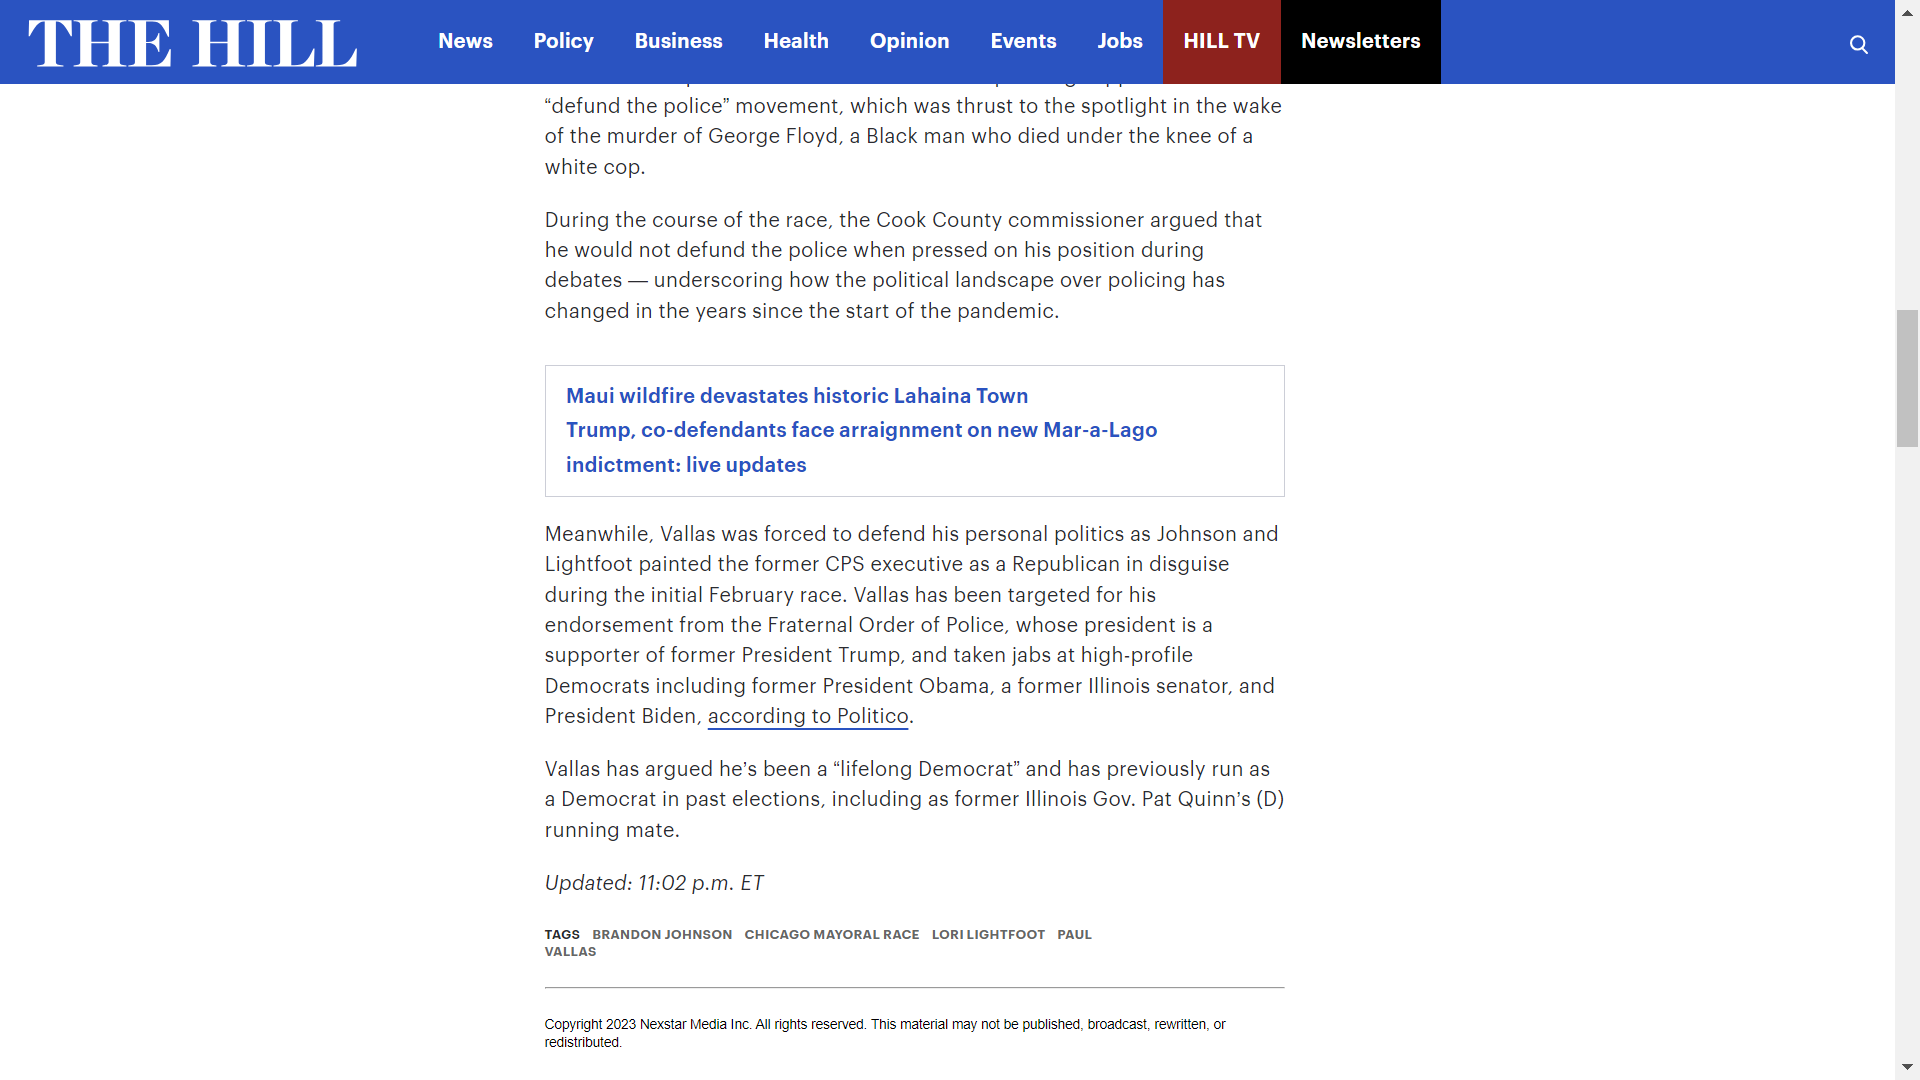
\includegraphics[width=0.75\textwidth]{gambar/bab_4_image/the-hill.png}
  \caption{Contoh \textit{tag} dari artikel thehill.com}
  \label{gambar:thehill}
\end{figure}

Untuk mendapatkan data-data seperti itu, penulis menggunakan 
\textit{crawler}. Dalam \emph{table} "\emph{page\_informations}", kolom yang dipakai 
nantinya adalah kolom \textit{id\_page}, \textit{content\_article}, 
dan \textit{title}. Kemudian, di dalam \textit{page\_tags}, 
kolom yang digunakan adalah kolom \textit{tag} dan \textit{page\_id}.  

% GAMBAR DATASET
\begin{figure}[H]
  \centering
  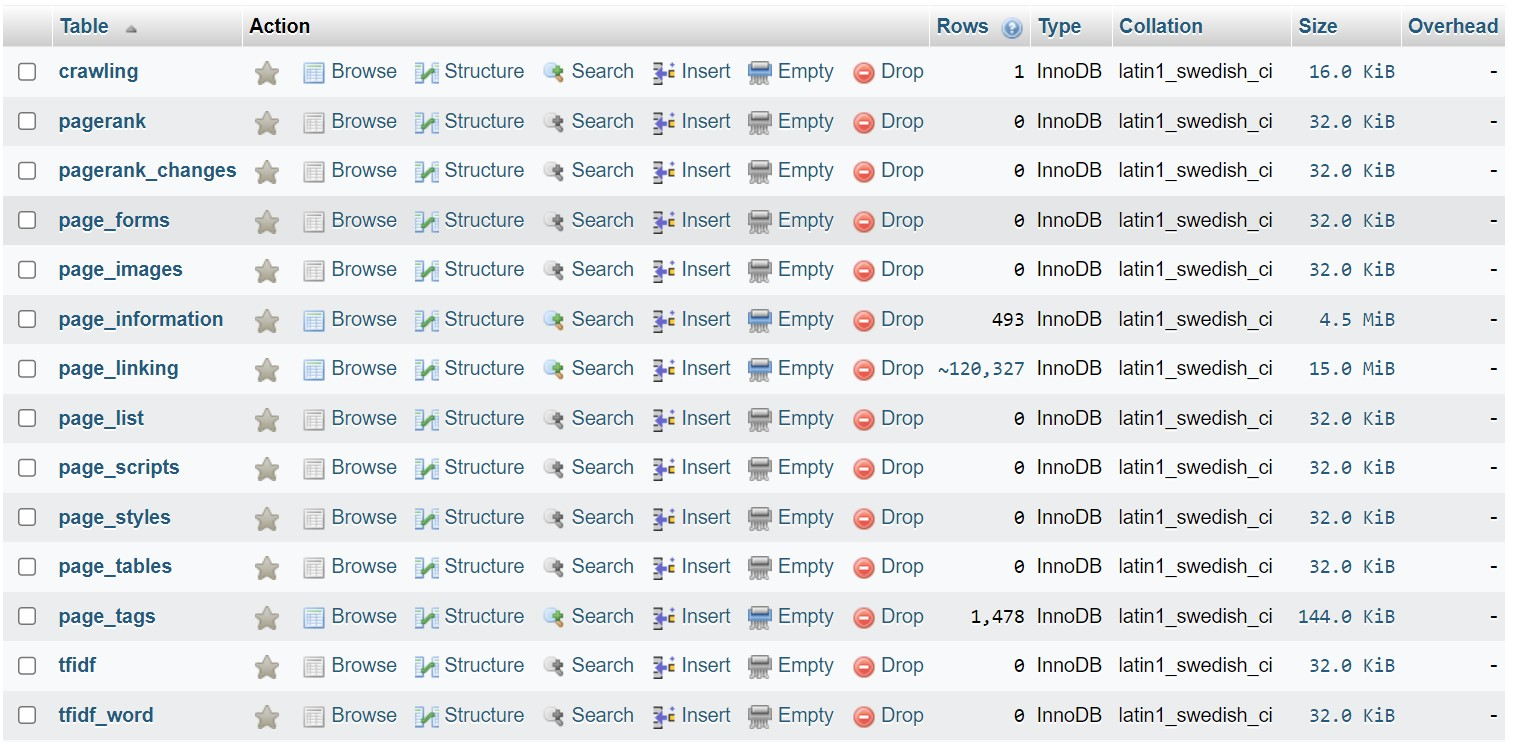
\includegraphics[width=0.75\textwidth]{gambar/bab_4_image/dataset.jpg}
  \caption{Dataset yang digunakan}
  \label{gambar:dataset}
\end{figure}

% GAMBAR DATASET TABLE PAGE tags
\begin{figure}[H]
  \centering
  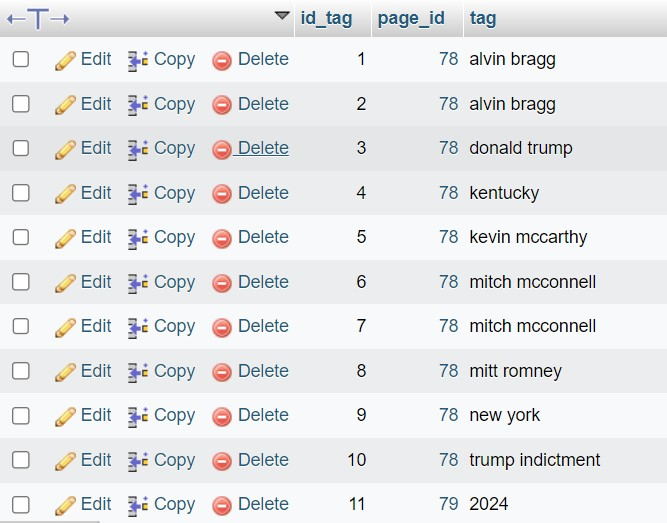
\includegraphics[width=1\textwidth]{gambar/bab_4_image/dataset tag.jpg}
  \caption{Dataset pada tabel \textit{page\_tags}}
  \label{gambar:datasetTag}
\end{figure}

% GAMBAR DATASET TABLE PAGE INFORMATION
\begin{figure}[H]
  \centering
  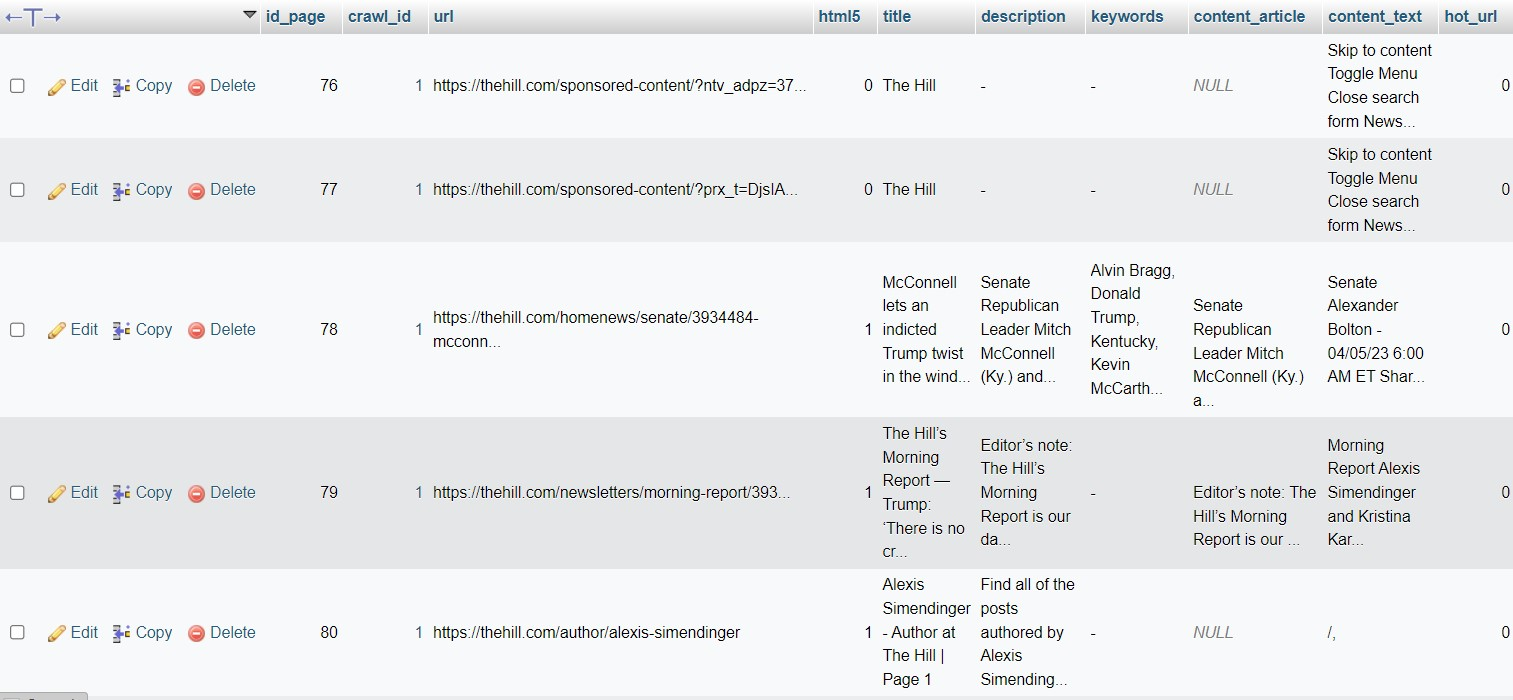
\includegraphics[width=1\textwidth]{gambar/bab_4_image/dataset article.jpg}
  \caption{Dataset pada tabel \textit{page\_informations}}
  \label{gambar:datasetInformation}
\end{figure}

\subsection{Pengambilan Data dari Database}

Data-data yang diambil adalah \emph{tag}, \emph{id} dari artikel, 
judul artikel, dan isi artikel melalui fungsi \emph{get\_data} 
pada \emph{file} \emph{data\_from\_database.py}.

% GAMBAR DARI HASIL PENGAMBILAN DATABASE

\begin{figure}[H]
  \centering
  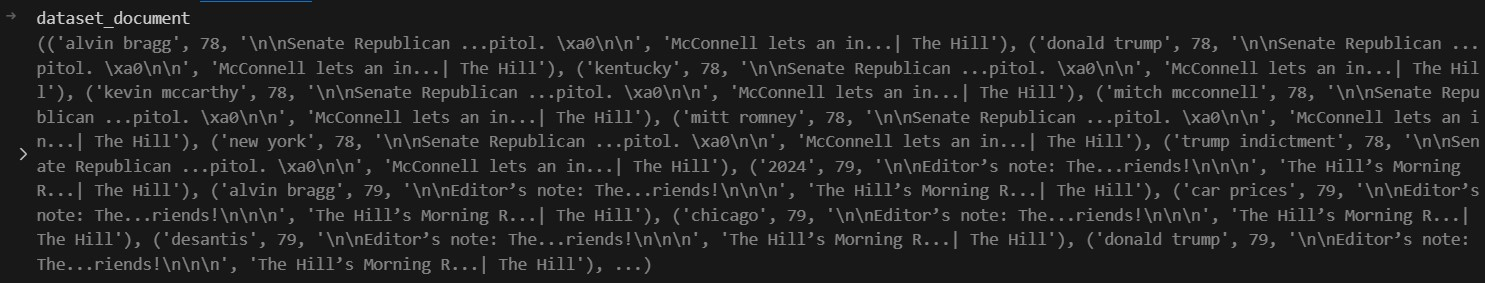
\includegraphics[width=1\textwidth]{gambar/bab_4_image/pengambilan data.jpg}
  \caption{Dataset yang digunakan}
  \label{gambar:pengambilanData}
\end{figure}

\subsection{Penginputan}

Untuk inputnya, $D$ didapat dari \textit{id} dan judul dari artikel yang ada. 
$T$ didapat dari \textit{tag} yang telah dikumpulkan. 
Lalu, $S$ didapat dari kata yang unik dari isi-isi artikel.
Selanjutnya, $K$ bernilai 2, $M$ bernilai 2, dan $L$ bernilai 2. 

\subsection{Mengolah Data Menjadi Matriks}

Data-data tersebut nantinya akan diolah menjadi matriks berdasarkan persamaan (\ref{w_ab}) 
yang di mana matriks $A$ adalah relasi antara \emph{tag} dengan dokumen dan 
matriks $B$ adalah relasi antara dokumen dengan \emph{word}. 
Untuk melakukan proses ini, diperlukan fungsi \emph{document\_processing} 
pada \textit{file} \textit{input\_processing.py}.

% GAMBAR HASIL OUTPUT DARI MATRIX A dan B
\begin{figure}[H]
  \centering
  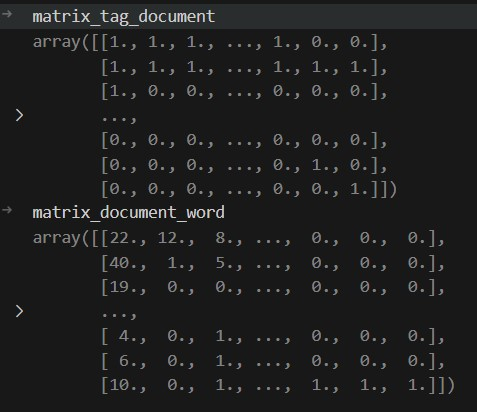
\includegraphics[width=0.75\textwidth]{gambar/bab_4_image/matrix tag document dan matrix document word.jpg}
  \caption{Matrix Tag Document dan Matrix Document Word}
  \label{gambar:matrixTagDocument}
\end{figure}

Lalu, kedua matriks tersebut disatukan hingga menjadi matriks $W$ 
berdasarkan persamaan (\ref{w_ab}) denggan menggunakan fungsi 
\textit{matrixABtoW} pada \textit{file} \textit{matrix\_processing.py}.

% GAMBAR HASIL OUTPUT MATRIX W
\begin{figure}[H]
  \centering
  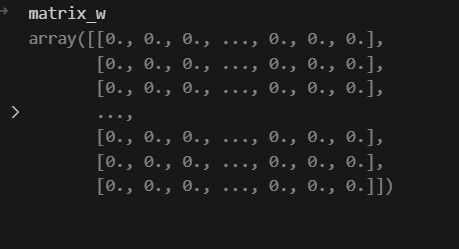
\includegraphics[width=0.75\textwidth]{gambar/bab_4_image/matrix w.jpg}
  \caption{Matrix W}
  \label{gambar:matrixW}
\end{figure}

\subsection{Menghitung Low Rank Approximation Matrix Menggunakan Algoritma Lanczos}

Untuk merubah matriks $W$ menjadi matriks $\tilde{W}$, diperlukan matriks
$Q_k$ dan $T_k$. Algoritma \textit{Lanczos Iteration} dapat digunakan untuk
mencari nilai dari matriks tersebut.

Dalam mencari nilai matriks $Q_k$ dan $T_k$, diperlukan \textit{function} 
\textit{lanczos\_iteration} pada \textit{file} \textit{low\_rank\_approximation\_matrix.py}.
Hasilnya adalah sebagai berikut.


% GAMBAR HASIL OUTPUT MATRIX Q DAN T
\begin{figure}[H]
  \centering
  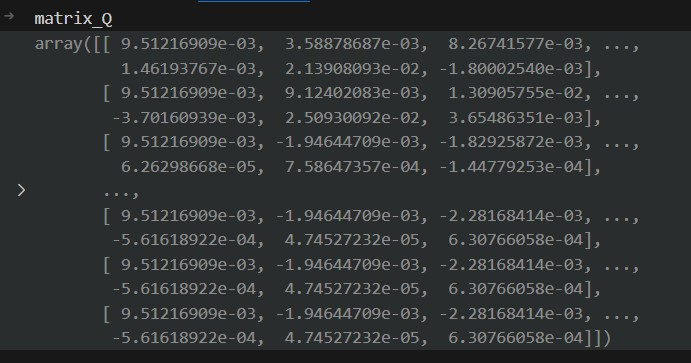
\includegraphics[width=0.75\textwidth]{gambar/bab_4_image/Matrix q.jpg}
  \caption{Matriks $Q$}
  \label{gambar:matrixQ}
\end{figure}

\begin{figure}[H]
  \centering
  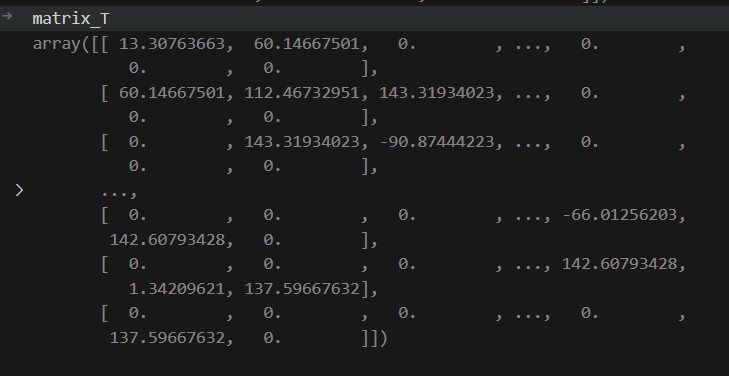
\includegraphics[width=0.75\textwidth]{gambar/bab_4_image/Matrix t.jpg}
  \caption{Matriks $T$}
  \label{gambar:matrixT}
\end{figure}

Selanjutnya, mencari nilai dari matriks $\tilde{W}$ dengan menggunakan \textit{function}
\textit{low\_rank\_approximation\_matrix} pada \textit{file} \textit{low\_rank\_approximation\_matrix.py}.
Hasilnya bisa dilihat di bawah ini.
% GAMBAR HASIL OUTPUT MATRIX W_hat

\begin{figure}[H]
  \centering
  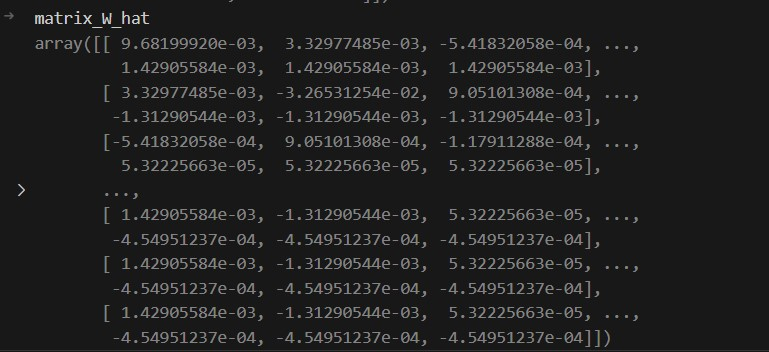
\includegraphics[width=0.75\textwidth]{gambar/bab_4_image/matrix w hat.jpg}
  \caption{Matriks $\tilde{W}$}
  \label{gambar:matrixWHat}
\end{figure}

\subsection{Melakukan Partisi W ke dalam Klaster K}

Agar dapat melakukan \textit{Bipartite Graph Partition}, perlu algoritma 
bernama \textit{Spectral Recursive Embedding}. Hasil dari partisi ini adalah
membentuk dua \textit{graph} terbaru dalam bentuk matriks. Untuk partisinya,
ditentukan oleh banyaknya $K$ yang telah diatur. Partisi ini menggunakan
fungsi \textit{spectral\_recursive\_embedding} pada \textit{file} 
\textit{spectral\_recursive\_embedding.py}.

% GAMBAR HASIL OUTPUT MATRIKS PARTITION
\begin{figure}[H]
  \centering
  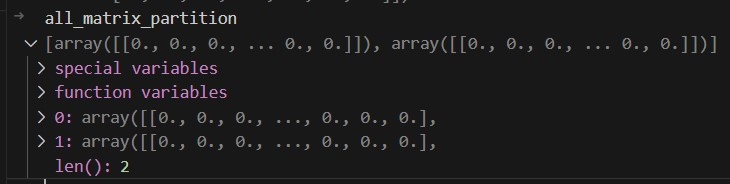
\includegraphics[width=1\textwidth]{gambar/bab_4_image/matrix partisi.jpg}
  \caption{Matriks hasil partisi}
  \label{gambar:matriksPartisi}
\end{figure}

\subsection{Melakukan Pelabelan Setiap Dokumen}

Setiap dokumen dilabelkan berdasarkan hasil partisi yang telah dilakukan.
Pelabelan ini tergantung banyaknya klaster yang disediakan. Jika terdiri
dari dua klaster, berarti dokumen tersebut akan dimasukkan ke dalam klaster
pertama atau klaster kedua sesuai hasil dari \textit{Bipartite Graph Partition} dengan
menggunakan fungsi \textit{assign\_label\_cluster} pada \textit{file}
\textit{assign\_label.py}.

% GAMBAR HASIL PELABELAN DOKUMEN
\begin{figure}[H]
  \centering
  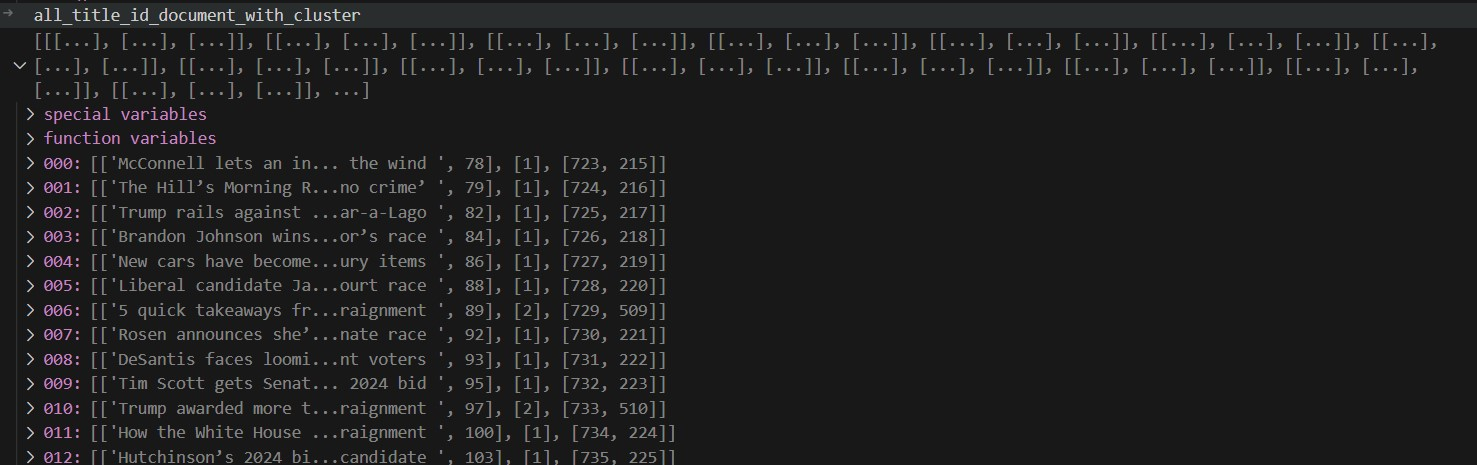
\includegraphics[width=1\textwidth]{gambar/bab_4_image/pelabelan dokumen.jpg}
  \caption{Pelabelan dokumen}
  \label{gambar:pelabelanDokumen}
\end{figure}

Pada variabel \textit{all\_title\_id\_document\_with\_cluster}, terdapat beberapa data di setiap \textit{index}.
Data tersebut yaitu
\begin{enumerate}
  \item Judul dokumen dan \textit{id}.
  \item Label klaster.
  \item \textit{Node} keberapa dalam suatu \textit{bipartite graph}.
\end{enumerate}

\subsection{Menghitung Rank(T) untuk setiap Tag}

Setiap \textit{tag} yang ada di dataset, perlu dihitung terlebih dahulu nilai
\textit{Rank(T)}. Untuk menghitung \textit{Rank(T)}, akan menggunakan fungsi
\textit{node\_rankt} dalam \textit{file} \textit{node\_rank\_t.py}. Hasilnya
sebagai berikut.

% GAMBAR RANK T

\begin{figure}[H]
  \centering
  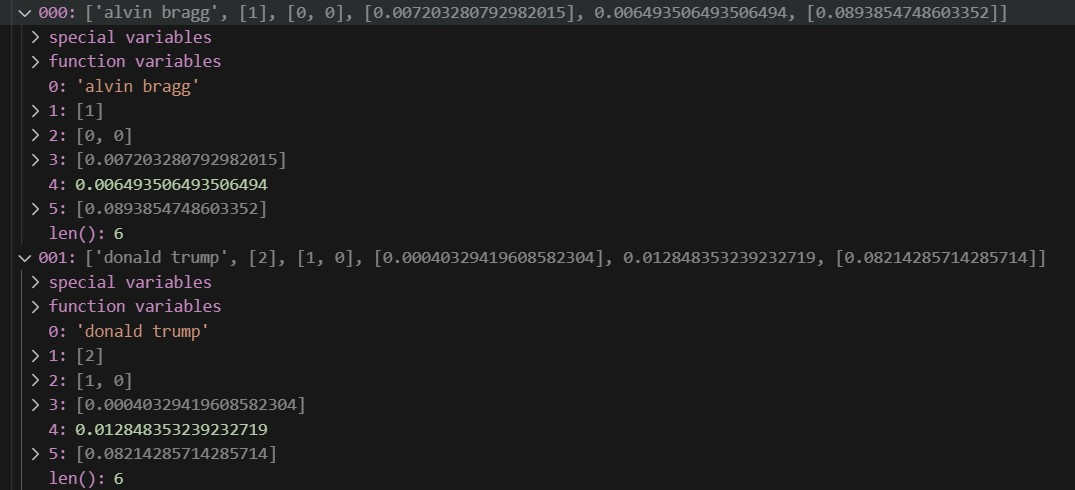
\includegraphics[width=1\textwidth]{gambar/bab_4_image/Node Rank T.jpg}
  \caption{Rank(T)}
  \label{gambar:rankT}
\end{figure}

Dari hasil ini, terdapat dua \textit{tag} yang digunakan sebagai contoh yaitu 
\textit{Alvin Bragg} dan \textit{Donald Trump}. \textit{Alvin Bragg} memiliki nilai 
\textit{N Precision} sebesar 0,893855 , \textit{N Recall} sebesar 0,006494, dan
\textit{Rank(T)} sebesar 0,007203. 

\subsection{Membuat Two Way Poisson Mixture Model}

Dalam membuat \textit{Two Way Poisson Mixture Model}, terdapat beberapa hal yang
diperlukan yaitu relasi antara dokumen dengan \textit{word vocabulary},
banyaknya komponen $M$, banyaknya klaster $K$, dan banyaknya 
\textit{word cluster} $L$.

Awalnya, perlu mencari $\pi_{m}$ dengan cara menghitung seluruh dokumen dalam komponen $m$
dibagi dengan seluruh dokumen yang ada menggunakan fungsi 
\textit{first\_prior\_probability} pada \textit{file} \textit{two\_way\_poisson\_mixture\_model.py}. 
Dengan menggunakan banyaknya komponen $M$ berjumlah dua, menghasilkan hasil sebagai berikut.

\begin{figure}[H]
  \centering
  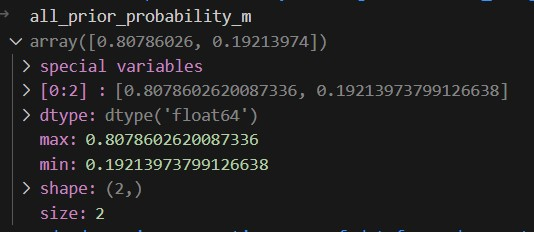
\includegraphics[width=0.75\textwidth]{gambar/bab_4_image/all_prior_probability_m.jpg}
  \caption{ $\pi_{m}$ }
  \label{gambar:priorProbability}
\end{figure}

Selanjutnya, mencari nilai $\tilde{\lambda_{m}}$ untuk setiap kata. Nilai $\tilde{\lambda_{m}}$
untuk setiap kata didapat dari nilai rata-rata kemunculan kata tersebut di setiap dokumen $d$
dalam setiap komponen $m$. Dengan menggunakan fungsi \textit{lambda\_m\_j\_list} pada \textit{file}
\textit{two\_way\_poisson\_mixture\_model.py} hasilnya sebagai berikut.

\begin{figure}[H]
  \centering
  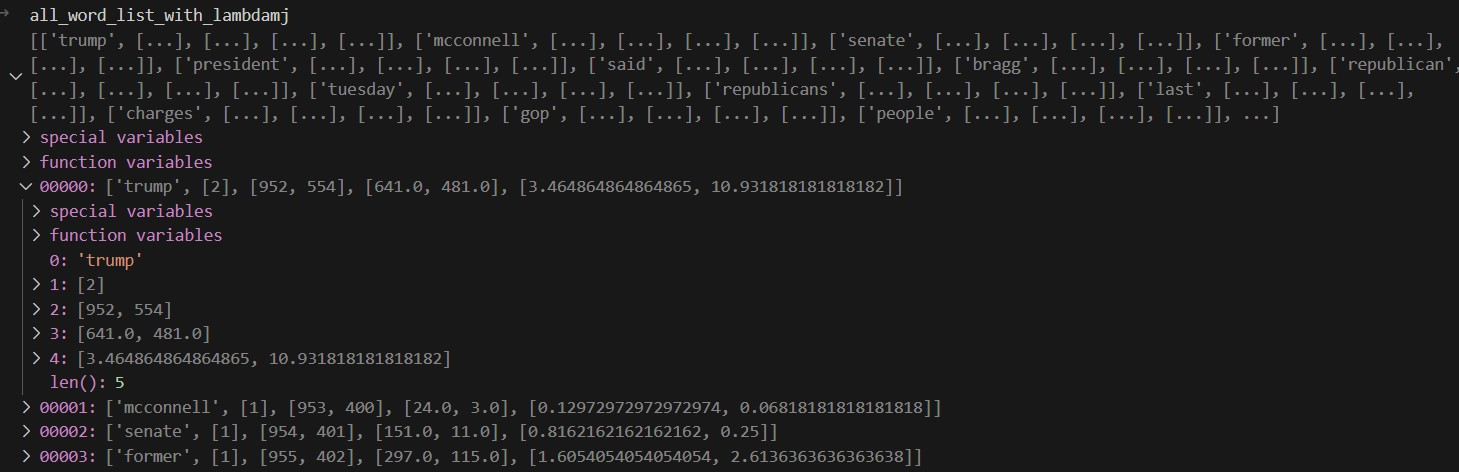
\includegraphics[width=1\textwidth]{gambar/bab_4_image/all word list lamda mj.jpg}
  \caption{ Daftar kata dengan nilai $\tilde{\lambda_{m}}$}
  \label{gambar:wordListLambdaMJ}
\end{figure}

Kemudian, mencari nilai $p_{i,m}$ dalam setiap dokumen untuk memulai fase \textit{E-step}  
dengan menggunakan fungsi \textit{p\_im\_list} pada \textit{file}
\textit{two\_way\_poisson\_mixture\_model.py}. Hasil yang didapat sebagai berikut.

\begin{figure}[H]
  \centering
  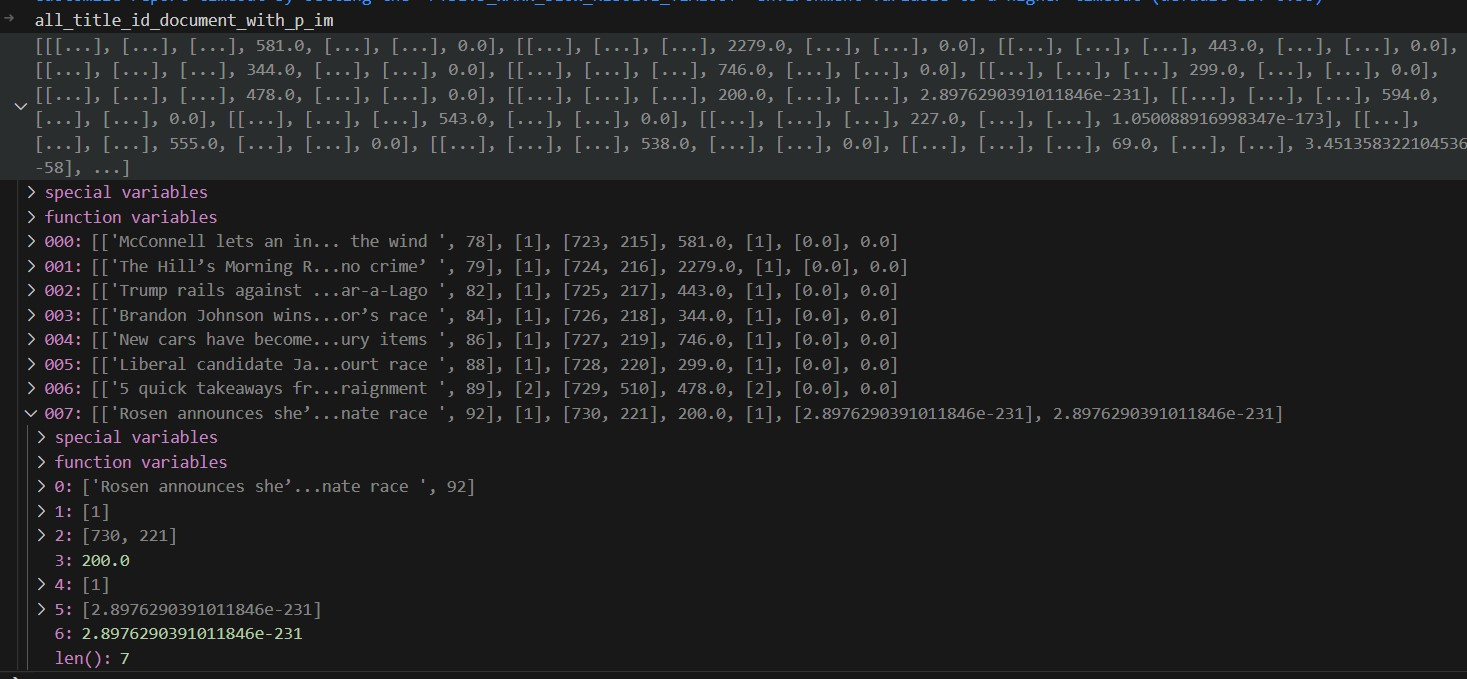
\includegraphics[width=0.75\textwidth]{gambar/bab_4_image/pim in document.jpg}
  \caption{Nilai $p_{i,m}$ pada setiap dokumen }
  \label{gambar:pim}
\end{figure}

Setiap \textit{index} dari variabel tersebut mengandung beberapa nilai yaitu
\begin{enumerate}
  \item Nilai dari judul dokumen dan \textit{id} dokumen.
  \item Klaster $k$ dari dokumen tersebut.
  \item \textit{Node} keberapa dari suatu \textit{bipartite graph} awal dan \textit{bipartite graph} setelah partisi.
  \item Banyaknya kata dalam dokumen.
  \item Komponen $m$ dari dokumen tersebut.
  \item Nilai dari $p_{i,m}$.
  \item Nilai dari $P(D=d|K=k)$ dari dokumen.
\end{enumerate}

Dari data di atas, nilai $p_{i,m}$ sangat rendah dan beberapa diantaranya 0. Hal ini dikarenakan perhitungan \textit{product}
dari nilai $\theta$ yang rendah, tapi nilai $p$ (banyaknya kata unik) yang banyak dalam persamaan \ref*{e_step}.

Selanjutnya adalah melakukan \textit{M-step}. Dalam penelitian ini, iterasi yang digunakan yaitu lima kali.

\subsection{Rekomendasi Tag}

Fungsi utama dari algoritma ini adalah membuat rekomendasi \textit{tag} berdasarkan
data latih yang tersedia. Saat ini, algoritma tersebut mampu memberikan sepuluh
pilihan \textit{tag} sesuai hasil rekomendasi. Dengan menggunakan fungsi
\textit{tag\_recommendation\_mass} pada \textit{file} \textit{tag\_recommendation\_for\_new\_document.py},
hasil yang didapat sebagai berikut.

% GAMBAR SALAH SATU CONTOH HASIL REKOMENDASI
\begin{figure}[H]
  \centering
  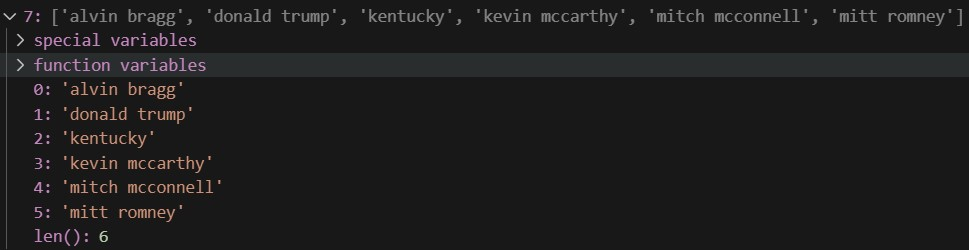
\includegraphics[width=1\textwidth]{gambar/bab_4_image/rekomendasi tag.jpg}
  \caption{Contoh dari hasil rekomendasi \textit{Tag}}
  \label{gambar:rekomendasiTag}
\end{figure}

\section{Hasil Pengujian}

Berdasarkan hasil pengujian, akurasi dari rekomendasi \textit{tag} 
dengan menggunakan algoritma \textit{Bipartite Graph Partition}
dan \textit{Two Way Poisson Mixture Model} adalah sebagai berikut.

% GAMBAR HASIL PENGUJIAN

\begin{figure}[H]
  \centering
  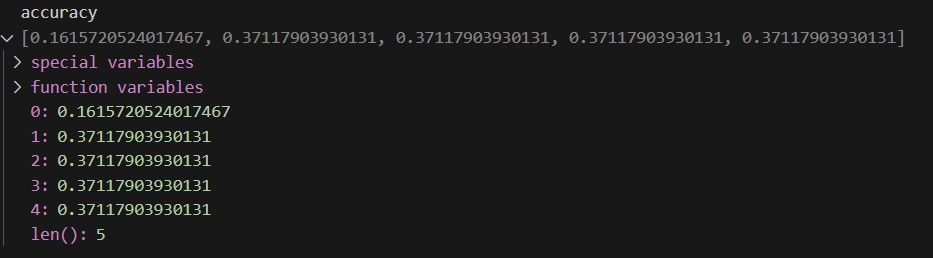
\includegraphics[width=1\textwidth]{gambar/bab_4_image/Akurasi.jpg}
  \caption{Contoh dari hasil rekomendasi \textit{Tag}}
  \label{gambar:akurasi}
\end{figure}

Saat melakukan iterasi di \textit{Poisson Mixture Model} sebanyak lima kali,
akurasi tertinggi sebanyak 37\% dengan jumlah data 229 dokumen dan 723 \textit{tag}.

Untuk pengujian ini, tidak menggunakan data uji dan justru melakukan pengujian dengan data yang sama
seperti data latih. 

\section{Hasil Analisa}

Berdasarkan hasil pengujian, jumlah akurasi terbilang sedikit yaitu 37,118\%. Tentunya, terdapat
beberapa faktor kenapa hasilnya rendah yaitu

\begin{enumerate}
  \item Penggunaan $K$ yang sangat sedikit saat melakukan \textit{Bipartite Graph Partition}.
  \item Nilai $P(D = d|K = k)$ yang terlalu sedikit juga menentukan rendahnya akurasi.
  \item Adanya kemungkinan hasil kodingan program yang kurang baik.
\end{enumerate}

Salah satu penyebabnya adalah saat perhitungan dengan menggunakan persamaan \ref*{e_step}. Dalam
melakukan perhitungan ini, nilai rata-rata pada $\theta \left(d(i, j) \mid \tilde{\lambda}_{m, i, j}^{(t)}\right)$
adalah sebagai berikut.

\begin{figure}[H]
  \centering
  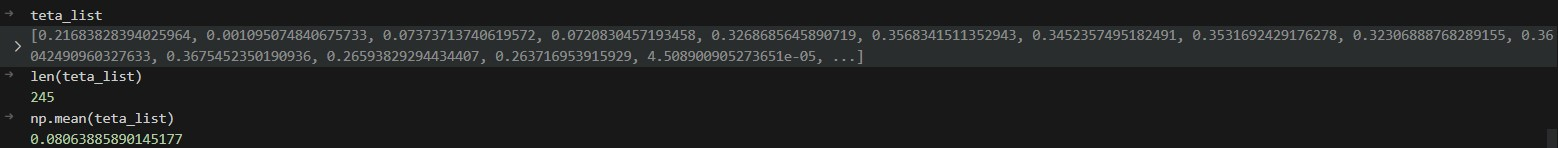
\includegraphics[width=1\textwidth]{gambar/bab_4_image/teta_list.jpg}
  \caption{Nilai $\theta \left(d(i, j) \mid \tilde{\lambda}_{m, i, j}^{(t)}\right)$}
  \label{gambar:teta_list}
\end{figure}

Selain itu, kelemahan kodingan program yang telah penulis buat adalah tidak bisa membagi \textit{Bipartite Graph Partition}
sesuai dengan sumber aslinya. Jika program yang penulis buat mampu membagi \textit{Bipartite Graph Partition} sesuai dengan
$K$ yang diinginkan, akurasinya bisa saja meningkat.


% - Hasil-hasil teta yang rendah
% - Tidak tersedianya bipartite graph partition jika K >= 2

% Spesifikasi Laptop yang digunakan.
% Implementasi code.
% Hasil berupa (database, dan isi database. peta graph).
%!TEX root = ./template-skripsi.tex
%-------------------------------------------------------------------------------
%                            	BAB IV
%               		KESIMPULAN DAN SARAN
%-------------------------------------------------------------------------------

\chapter{KESIMPULAN DAN SARAN}

\section{Kesimpulan}
Berdasarkan hasil dari implementasi dan pengujian \textit{Automatic Tagging} dengan 
menggunakan algoritma \textit{Bipartite Graph Partition} dan \textit{Two Way Poisson Mixture Model}
, maka diperoleh kesimpulan sebagai berikut. Program yang telah dibuat dapat menghasilkan beberapa rekomendasi \textit{tag}.
Akan tetapi, akurasi yang dihasilkan masih sangat rendah yaitu 37\%. Hal ini dikarenakan banyaknya $K$ yang digunakan dalam program ini
untuk melakukan \textit{Bipartite Graph Partition} hanyalah dua. Selain itu, nilai  $\theta \left(d(i, j) \mid \tilde{\lambda}_{m, i, j}^{(t)}\right)$
yang dihasilkan mempengaruhi nilai $p_{i,m}$.

\section{Saran}
Adapun saran untuk penelitian selanjutnya adalah:
\begin{enumerate} 
	\item Menggunakan jumlah $K$ yang lebih optimal.
	\item Menggunakan dataset yang lebih besar karena tingkat akurasinya 
	akan lebih meningkat dibandingkan dengan dataset yang lebih kecil.
	\item Dapat menggunakan bahasa Indonesia dalam pemilihan artikel atau situs 
	yang digunakan untuk penelitian. 
	\item Mengintegrasikan algoritma ini ke dalam aplikasi \textit{website} agar 
	pengguna mampu menggunakannya lebih mudah.
	\item Melakukan sinkronisasi dari algoritma \textit{Automatic Tagging} ke dalam 
	sistem mesin pencari \textit{Telusuri}.
\end{enumerate}


% Baris ini digunakan untuk membantu dalam melakukan sitasi
% Karena diapit dengan comment, maka baris ini akan diabaikan
% oleh compiler LaTeX.
\begin{comment}
\bibliography{daftar-pustaka}
\end{comment}

%-----------------------------------------------------------------
%Disini akhir masukan Bab
%-----------------------------------------------------------------


%-----------------------------------------------------------------
% Disini awal masukan untuk Daftar Pustaka
% - Daftar pustaka diambil dari file .bib yang ada pada folder ini
%   juga.
% - Untuk memudahkan dalam memanajemen dan menggenerate file .bib
%   gunakan reference manager seperti Mendeley, Zotero, EndNote,
%   dll.
%-----------------------------------------------------------------
\bibliographystyle{apalike}
\bibliography{daftar-pustaka}
\addcontentsline{toc}{chapter}{DAFTAR PUSTAKA}
%-----------------------------------------------------------------
%Disini akhir masukan Daftar Pustaka
%-----------------------------------------------------------------

% Lampiran ditaruh setelah Daftar Pustaka
\addcontentsline{toc}{chapter}{LAMPIRAN}
\appendix 
% \setlength{\parindent}{0.5in}
% \fontsize{6}

\lstset{
  basicstyle=\fontsize{9}{12}\selectfont, % Set your desired font size
	% Specify the programming language
  % ... other listing options ...
}

\chapter{main.py}
\begin{lstlisting}[breaklines=true]
# Source dari file
import data_from_database as dfd 
import matrix_processing as mp
import input_processing as ip
import normalized_laplacian as nl
import low_rank_approximation_matrix as lram
import spectral_recursive_embedding as sre
import the_moment as tm
import assign_label as al
import node_rank_t as nrt
import word_count_in_matrix as wcim
import two_way_poisson_mixture_model as twpmm
import word_count_in_list as wcil
import tag_recommendation_for_new_document as trfnd
import top_k_accuracy as tka
import data_testing_converter as dtc

import numpy as np

tm.this_moment("Menjalankan Algoritma :")

# Mengambil data dari database
dataset_document = dfd.get_data()
tm.this_moment("Mengambil dataset :")

# Mensetting K, M, dan L
K = 2
M = 2
L = 2

# Memproses dataset menjadi matrix
matrix_tag_document, matrix_document_word, title_id_document, all_tag_list, all_word_list, dataframe_document_tag, dataframe_document_word = ip.document_processing(dataset_document)
tm.this_moment("dataset ke matrix :")

matrix_w = mp.matrixABtoW(matrix_tag_document, matrix_document_word)
tm.this_moment("matrix A & B menjadi W :")

matrix_Q, matrix_T = lram.lanczos_iteration(matrix_w, 1)
matrix_W_hat = lram.low_rank_approximation_matrix(matrix_Q, matrix_T)
tm.this_moment("Low Rank Approximation :") 
# print(matrix_W_hat)

all_matrix_partition, all_cluster = sre.spectral_recursive_embedding(matrix_W_hat, matrix_w)
tm.this_moment("Spectral Recursive Embedding :")
# print("X")

all_matrix_w_hat_partition = []
for matrix_partition in all_matrix_partition:
	Q, T = lram.lanczos_iteration(matrix_partition, 1)
	matrix_W_hat_partition = lram.low_rank_approximation_matrix(Q, T)
	all_matrix_w_hat_partition.append(matrix_W_hat_partition)
tm.this_moment("Create W hat partition :")

all_tag_list_with_cluster, all_title_id_document_with_cluster, all_word_list_with_cluster = al.assign_label_cluster(title_id_document, all_tag_list, all_word_list, all_cluster)
tm.this_moment("Assign Label :")

all_tag_list_with_rank = nrt.node_rankt(all_tag_list_with_cluster, matrix_w, all_matrix_partition)
tm.this_moment("Node Rank T :")

# Menghitung banyaknya document dari 
all_title_id_document_with_word_count, total_doc, total_doc_in_cluster = wcim.word_count_in_matrix(all_title_id_document_with_cluster, all_matrix_partition, dataframe_document_word)
tm.this_moment("Word Count setiap Document dari Matrix partisi :")
# print("X")

# Menghitung banyaknya word serta banyaknya word di masing-masing klaster
all_word_list_with_count, total_word, total_word_in_cluster = wcil.word_count_in_list(all_word_list_with_cluster, matrix_w, all_matrix_partition)
tm.this_moment("Word Count setiap word :")

# Two Way Poisson Mixture Model
# Memilih m component
all_title_id_document_with_m_component, total_doc_in_component = twpmm.set_m_component_to_document(all_title_id_document_with_word_count, M ,K)
tm.this_moment("Menentukan m component pada suatu klaster :")

# Menghitung banyaknya word serta banyaknya word di masing-masing komponen
all_word_list_with_count = twpmm.set_word_count_in_every_m(all_title_id_document_with_m_component, all_word_list_with_count, M, K, matrix_document_word)
tm.this_moment("Word Count setiap word :")
# Menghitung prior probability
all_prior_probability_m = twpmm.first_prior_probability(total_doc, total_doc_in_component)
tm.this_moment("prior probability :")
# Menghitung nilai lambda
all_word_list_with_lambdamj = twpmm.lambda_m_j_list(all_word_list_with_count, total_doc_in_component)
tm.this_moment("lambda(m,j) :")
# Menghitung probabilitas
all_title_id_document_with_probability = twpmm.probability(all_title_id_document_with_m_component, all_prior_probability_m, all_word_list_with_lambdamj, dataframe_document_word, M)
tm.this_moment("P(D = d|C = k) :")
# Menghitung nilai p(i,m)
all_title_id_document_with_p_im = twpmm.p_im_list(all_title_id_document_with_probability, all_prior_probability_m, all_word_list_with_lambdamj, dataframe_document_word, M)
tm.this_moment("p(i,m) :")

# Looping Expectation Maximization
log_likelihood = []
top_k_accuracy_list = []
for i in range(1, 6):
	# Menghitung Prior probability (pi_m) t+1
	all_prior_probability_m, sum_p_im_list = twpmm.pi_m_with_t(all_title_id_document_with_p_im, M)
	tm.this_moment("pi(m) (t+1) :")
	# Menghitung lambda t+1
	all_word_list_with_lambdamj = twpmm.lambda_mt(all_word_list_with_lambdamj, sum_p_im_list, all_title_id_document_with_p_im, M)
	tm.this_moment("lambda(m) (t+1) :")
	# Menghitung nilai likelihood
	new_all_title_id_document_with_p_im = twpmm.p_im_list_t_more_than_1(all_title_id_document_with_p_im, all_prior_probability_m, all_word_list_with_lambdamj, dataframe_document_word)
	tm.this_moment("p(i,m) (t+1) :")
	log_likelihood.append(twpmm.get_log_likelihood(all_title_id_document_with_p_im, new_all_title_id_document_with_p_im))
	all_title_id_document_with_p_im = new_all_title_id_document_with_p_im
	all_title_id_document_with_probability = twpmm.set_new_probability_t(all_title_id_document_with_p_im)
	tm.this_moment("Menghitung nilai Log Likelihood :")

	all_title_id_document_with_tag_recommendation = trfnd.tag_recommendation_mass(all_title_id_document_with_probability, all_tag_list_with_rank, all_cluster, total_doc_in_cluster)
	tm.this_moment('Tag Recommendation: ')

	top_k_accuracy_value = tka.top_k_accuracy(all_title_id_document_with_tag_recommendation, dataframe_document_tag)
	tm.this_moment('Top 6 Tag: ')
	
	top_k_accuracy_list.append(top_k_accuracy_value)

accuracy = []
for tkal in top_k_accuracy_list:
	accuracy.append(tkal.count(1) / len(tkal))

tm.this_moment('Menghitung akurasi: ')

print("X")
	
	
\end{lstlisting}

\chapter{data\textunderscore from\textunderscore database.py}
\begin{lstlisting}[breaklines=true]
import pymysql.cursors

connection = pymysql.connect(host='localhost', user='root', password='', database='autotag-crawl', autocommit=True,)

# Mengambil data dari database
def get_data():
	with connection:
		with connection.cursor() as cursor:
				
			# Mengambil data tag, title, dan isi artikel
			cursor.execute("SELECT DISTINCT page_tags.tag, page_information.id_page, page_information.content_article, page_information.title FROM `page_tags` INNER JOIN page_information ON page_tags.page_id = page_information.id_page")
			result = cursor.fetchall()
			return result

\end{lstlisting}

\chapter{input\textunderscore processing.py}
\begin{lstlisting}[breaklines=true]
import nltk
import numpy as np
import pandas
import re
import the_moment as tm

from nltk.corpus import stopwords
from nltk.tokenize import word_tokenize

unique_words = []
words = []
tags = []
documents = []

def wordProcessing(content_article):
	"""
	Fungsi untuk menghitung banyaknya word dalam suatu artikel

	Args:
		content_article: Isi dari artikel
	
	Sumber library untuk menghitung kata:
		https://www.nltk.org/book/ch01.html
		
	Returns:
			word_document_dictionary: berupa dictionary untuk menghitung banyaknya 
		dan beragamnya word dalam suatu document
	"""
	tokens = word_tokenize(re.sub('[^ 0-9a-z]+', ' ', content_article.lower())) # Menghilangkan tanda baca   
	english_stopwords = stopwords.words('english') # Menampilkan daftar stopwords
	english_stopwords.extend(['a', 'b', 'c', 'd', 'e', 'f', 'g', 'h', 'i', 'j', 'k', 'l', 'm', 'n', 'o', 'p', 'q', 'r', 's', 't', 'u', 'v', 'w', 'x', 'y', 'z']) #menambahkan stopwords
	tokens_wo_stopwords = [t for t in tokens if t not in english_stopwords] 

	# Menghitung banyaknya word
	freq = nltk.FreqDist(tokens_wo_stopwords)
	word_document_dictionary = {}

	# Menampung word tersebut dalam format dictionary
	# Alasan menggunakan freq.most_common(2000) untuk mendapatkan 2000 kata yg sering muncul
	for word, count in freq.most_common(2000):
			word_document_dictionary.update({word: count})
	
	unique_words.append(len(word_document_dictionary))
	words.append(len(tokens_wo_stopwords))
	# len(word_document_dictionary)
			
	# print("Dictionary : ", word_document_dictionary)
	return word_document_dictionary

def documentWordProcessing(content_article):
		"""
		Fungsi untuk membuat dataframe antara document(title) dengan word

		Args:
			content_article: Isi dari artikel
			id_article: ID dari artikel

		Returns:
				word_document: word_document dalam bentuk dataframe
		"""
		word_document_dictionary = wordProcessing(content_article)
		# word_document = pandas.DataFrame(word_document_dictionary,
		#     index=[id_article]
		# )
		return word_document_dictionary

def document_processing(dataset_document):
	"""
	Memproses dataset yang masuk, lalu mengolahnya menjadi kumpulan dataframe antara tag dgn dokumen
	dan dokumen dgn word

	Args:
		dataset_document: data-data yg diambil dari database dengan isi "tag, id_article, content_article"
		
	Returns:
		matrix_tag_document: matriks antara tag dgn document
		matrix_document_word: matriks antara document dgn word
		title_id_document: relasi antara title dan id dari suatu artikel
	"""
	
	# tm.this_moment('Mulai Document Processing :')
	id_before = dataset_document[0][1]
	# document_word = []
	# document_word.append(documentWordProcessing(dataset_document[0][2], dataset_document[0][1]))
	
	title_id_document = []
	title_id_document.append((dataset_document[0][3].replace('| The Hill', ''), dataset_document[0][1]))
	
	tag_dictionary = {}
	tag_dictionary_list = []
	
	word_dictionary = {}
	word_dictionary_list = []
	word_dictionary_list.append(documentWordProcessing(dataset_document[0][2]))
	
	id_list = []
	# Tempat untuk menghitung banyaknya tag dalam suatu dokumen
	document_tag = []
	
	# tm.this_moment('Mulai looping :')
	for data in dataset_document:
		
		# Jika judul data berbeda dengan id_before
		if id_before != data[1]:
			
			# Menampung tag-tag yg telah didapat di tag_dictionary ke document_tag
			id_list.append(id_before)
			tag_dictionary_list.append(tag_dictionary.copy())
			tags.append(len(tag_dictionary.copy()))
			# document_tag.append(datafr)
			tag_dictionary.clear()
			
			# Melakukan proses untuk menghitung banyaknya kata dalam suatu dokumen
			title_id_document.append((data[3].replace('| The Hill', ''), data[1]))
			word_dictionary_list.append(documentWordProcessing(data[2]))
			id_before = data[1]
		
		#tag yg didapat akan dimasukkan ke tag_dictionary
		tag_dictionary.update({data[0]: 1})

	id_list.append(id_before)
	tag_dictionary_list.append(tag_dictionary.copy())
	tags.append(len(tag_dictionary.copy()))
	tag_dictionary.clear()
	
	# tm.this_moment('Mulai concat docword :')
	document_word = pandas.DataFrame(word_dictionary_list, index=id_list)
	document_word = document_word.fillna(0)
	
	# tm.this_moment('Mulai concat doctag :')
	document_tag = pandas.DataFrame(tag_dictionary_list, index=id_list)
	document_tag = document_tag.fillna(0)

	
	# tm.this_moment('Mulai membuat matrix :')
	matrix_tag_document = document_tag.to_numpy().transpose()
	matrix_document_word = document_word.to_numpy()
	return matrix_tag_document, matrix_document_word, title_id_document, document_tag.columns, document_word.columns, document_tag, document_word

\end{lstlisting}

\chapter{matrix\textunderscore processing.py}
\begin{lstlisting}[breaklines=true]
import numpy as np

def matrixABtoW(A, B):
	"""
	Fungsi untuk menggabungkan matriks A dan B menjadi W

	Args:
		A: Matriks A dengan tag sebagai row dan document sebagai column
		B: Matriks B dengan document sebagai row dan word sebagai column

	Returns:
		W: Matriks gabungan antara A dengan B
	"""
	AT = A.transpose()
	BT = B.transpose()

	# Menghitung banyaknya tag, dokumen, dan word
	tag_count, document_count = A.shape
	document_count, word_count = B.shape

	# Membuat matriks W dengan panjang dan lebar dari "tag + dokumen + word"
	all_count = tag_count + document_count + word_count
	W = np.zeros((all_count, all_count))

	# Menempelkan matriks A ke W
	for i in range(tag_count):
		W[i][tag_count:-word_count] = A[i]

	# Menempelkan matriks B Transpose ke W
	for i in range(1, word_count+1):
		W[-i][tag_count:-word_count]= BT[-i]

	# Menempelkan matriks A Transpose ke W
	for i in range(document_count):
		W[tag_count+i][0:tag_count] = AT[i]
			
	# Menempelkan matriks B ke W
	for i in range(document_count):
		W[tag_count+i][-word_count:] = B[i]
	
	return W
\end{lstlisting}

\chapter{low\_rank\_approximation\_matrix.py}
\begin{lstlisting}[breaklines=true]
import numpy as np

def normalization_vector(vector):
	vector_power = [np.power(x, 2) for x in vector]
	vector_normalize = np.sqrt(np.sum(vector_power))
	return vector_normalize

def lanczos_iteration(A, one_b = 1):
	"""
	Melakukan Lanczos iteration dengan membuat matriks Q dan T
	Kemudian, membuat kedua matriks tersebut menjadi W_hat

	Args:
		A: Inputan dari matriks W
		
	Returns:
		Q: Hasil perkalian matriks Q 
	"""
	
	k = 50
	
	row, column = A.shape
	
	# Buat matriks T untuk menampung alpha dan beta
	T = np.zeros((k, k))
	
	# buat matriks Q untuk menampung q_now di setiap looping
	Q = np.zeros((row, k))
	
	beta = 0 
	q_before = 0
	b = "" # Bentuk matriks b secara arbitrary (bebas)
	if (one_b != 1):
		b = np.random.default_rng().random((row, 1))
	else:
		b = np.ones((row, 1)) 
		
	# Matriks q_now adalah matriks yg telah normalisasi
	# panjang q_now = 1, cek panjang q_now dengan np.sqrt(np.sum([x*x for x in q_now]))
	q_now = b / normalization_vector(b)
	
	Q[:, 0] = q_now.transpose()
	
	for i in range(1, k):
		v = A.dot(q_now)
		alpha = q_now.transpose().dot(v)
		alpha = alpha[0][0] # Membuat alpha agar menjadi skalar
		v = v - beta*q_before - alpha*q_now
		beta = normalization_vector(v)
		q_before = q_now
		q_now = v / beta
		
		# Tampung alpha dan beta ke matriks T
		T[i-1, i-1] = alpha
		if i < row:
			T[i-1, i] = beta
			T[i, i-1] = beta
			
			# Tampung nilai q_now ke matriks Q
			Q[:, i] = q_now.transpose()

	return Q, T

def low_rank_approximation_matrix(Q, T):
	"""
	Melakukan perkalian matriks Q, T, dan Q transpose

	Args:
		Q: Matriks Q yang didapat dari Lanczos iteration
		T: Matriks T yang didapat dari Lanczos iteration
		
	Returns:
		W_hat: Hasil perkalian matriks Q, T, dan Q transpose
	"""
	
	return Q.dot(T).dot(Q.transpose())
\end{lstlisting}

\chapter{spectral\_recursive\_embedding.py}
\begin{lstlisting}[breaklines=true]
import numpy as np
import scipy as sp
import normalized_laplacian as nl
import matrix_processing as mp
import low_rank_approximation_matrix as lram

import the_moment as tm

def second_largest_singular_vector(W_hat):
	"""
		Menghitung singular vector menggunakan W_hat dari library
		https://docs.scipy.org/doc/scipy/reference/sparse.linalg.svds-lobpcg.html    
		
		Args:
			W_hat: Matrix W_hat

		Returns:
			second_largest_left: Mengambil vektor U
			second_largest_right: Mengambil vektor Vh
	"""
	
	U, s, Vh = sp.sparse.linalg.svds(W_hat, solver='lobpcg')
	# U, s, Vh = sp.linalg.svd(W_hat)
	second_largest_left = U[:, 1] # Mengambil left singular vector kedua
	second_largest_right = Vh[1, :] # Mengambil right singular vector kedua
	
	return second_largest_left, second_largest_right

def find_cut_point(singular_vector_left, singular_vector_right ):
	"""
		Mencari cut point

		Returns:
			cx: cx
			cy: cy
	"""
	
	cx = np.median(singular_vector_left)  
	cy = np.median(singular_vector_right) 
	return cx, cy

def form_partition(cx, cy, x, y):
	"""
		Melakukan form partition
		
		Args:
			cx: cut point untuk x
			cy: cut point untuk y
			x: Hasil dari second_largest_left
			y: Hasil dari second_largest_right
			
		Returns:
			A_partition
			Ac_partition
			B_partition
			Bc_partition
	"""
	
	A_partition = []
	Ac_partition = []
	B_partition = []
	Bc_partition = []

	i = 0
	for value in x:
		if value >= cx:
			A_partition.append(i)
		else:
			Ac_partition.append(i)
		i+=1

	j = 0
	for value in y:
		if value >= cy:
			B_partition.append(j)
		else:
			Bc_partition.append(j)
		j+=1
	
	return A_partition, Ac_partition, B_partition, Bc_partition


def create_matrix_from_two_vertex(X, Y, W):
	"""
		Menggabungkan dua partisi ke dalam satu matrix berdasarkan
		'Bipartite graph partitioning and data clustering'

		Args:
			X: Vertex x
			Y: Vertex y
			W: Matrix W awal

		Returns:
			matrix: Matrix dari bipartite graph yg terbaru
			XY: Tanda untuk pada vertex keberapa ia di klaster ini
	"""
	
	XY = list(set(X).union(set(Y)))
	len_xy = len(XY)
	matrix = np.zeros((len_xy , len_xy))
	
	# Looping untuk membuat matrix_w hasil partisi
	for i in range(0, len_xy):
		xy_i = XY[i]
		for j in range(0, len_xy):
			xy_j = XY[j]
			matrix[i][j] = W[xy_i][xy_j]
	
	return matrix, XY

def spectral_recursive_embedding(W_hat, W):
	"""
		Melakukan bipartite graph partition dengan menggunakna
		spectral recursive embedidng

		Args:
			W_hat: Matrix W_hat
			Y: Vertex y
			W: Matrix W awal

		Returns:
			all_matrix: List Matrix w hasil klasterisasi
			all_cluster: Klaster
	"""
	all_matrix = []
	all_cluster = []
	# tm.this_moment("Start :")
	x, y = second_largest_singular_vector(W_hat)
	# tm.this_moment("Second Largest Singular Vector :")
	cx, cy = find_cut_point(x, y)
	# tm.this_moment("Cut Point :")
	A, Ac, B, Bc = form_partition(cx, cy, x, y)
	# tm.this_moment("Form Partition :")
	matrix, cluster = create_matrix_from_two_vertex(A, B, W)
	all_matrix.append(matrix)
	all_cluster.append(cluster)
	matrix, cluster = create_matrix_from_two_vertex(Ac, Bc, W)
	all_matrix.append(matrix)
	all_cluster.append(cluster)
	# tm.this_moment("Fusion the matrix :")
	
	return all_matrix, all_cluster
\end{lstlisting}

\chapter{assign\_label.py}
\begin{lstlisting}[breaklines=true]
def assign_label_for_tag(all_tag_list, all_cluster, index):
  all_tag_list_with_cluster = []
  
  # Looping seluruh isi all_tag_list
  for tag in all_tag_list:
    tag_cluster = []
    tag_index_in_matrix = [] # Kumpulan index dalam satu tag di dalam setiap matrix yg ditempati tag tersebut
    index_cluster = 0 # index klaster
    
    tag_index_in_matrix.append(index)
    # Looping selurung klaster
    for cluster in all_cluster:
      if index in cluster:
        tag_cluster.append(index_cluster + 1)
        tag_index_in_matrix.append(cluster.index(index))
      index_cluster+=1
      
    index += 1
    all_tag_list_with_cluster.append([tag, tag_cluster, tag_index_in_matrix])
  
  return index, all_tag_list_with_cluster
  
def assign_label_for_document(title_id_document, all_cluster, index):
  # Memasukkan label klaster ke dalam document
  all_title_id_document_with_cluster = []
  
  # Looping seluruh isi title_id_document
  for title, id in title_id_document:
    document_cluster = []
    document_index_in_matrix = [] # Kumpulan index dalam satu document di dalam setiap matrix yg ditempati document tersebut
    index_cluster = 0

    document_index_in_matrix.append(index)
    # Looping isi klaster
    for cluster in all_cluster:
      # Jika index tersebut ada di suatu klaster
      if index in cluster:
        document_cluster.append(index_cluster + 1)
        document_index_in_matrix.append(cluster.index(index))
      index_cluster+=1

    index += 1
    all_title_id_document_with_cluster.append([[title, id], document_cluster, document_index_in_matrix])

  return index, all_title_id_document_with_cluster

def assign_label_for_word(all_word_list, all_cluster, index):
  # Memasukkan label klaster ke dalam word
  all_word_list_with_cluster = []
  
  # Looping seluruh word di all_word_list
  for word in all_word_list:
    word_cluster = []
    word_index_in_matrix = [] # Kumpulan index dalam satu word di dalam setiap matrix yg ditempati word tersebut
    index_cluster = 0
    
    word_index_in_matrix.append(index)
    # Looping isi klaster
    for cluster in all_cluster:
      if index in cluster:
        word_cluster.append(index_cluster + 1)
        word_index_in_matrix.append(cluster.index(index))
      index_cluster+=1

    index += 1
    all_word_list_with_cluster.append([word, word_cluster, word_index_in_matrix])
  
  return index, all_word_list_with_cluster

def assign_label_cluster(title_id_document, all_tag_list, all_word_list, all_cluster): 
  
  # Memasukkan label klaster ke dalam tag
  index = 0 # Index row matrix awal
  index, all_tag_list_with_cluster = assign_label_for_tag(all_tag_list, all_cluster, index)
  index, all_title_id_document_with_cluster = assign_label_for_document(title_id_document, all_cluster, index)
  index, all_word_list_with_cluster = assign_label_for_word(all_word_list, all_cluster, index)

  return all_tag_list_with_cluster, all_title_id_document_with_cluster, all_word_list_with_cluster
\end{lstlisting}

\chapter{node\_rank\_t.py}
\begin{lstlisting}[breaklines=true]
import numpy as np

import matrix_processing as mp

def n_recall(matrix_w_origin, matrix_w_partition, node_i_origin):
	"""
		Menghitung N Precision dari suatu tag

		Args:
			matrix_w_origin: matrix w yg dari awal dibuat
			tag_cluster: 
			node_i_origin: node di matrix w yg dari awal dibuat

		Returns:
			nri: N Recall dari suatu tag
	"""
	
	row, col = matrix_w_partition.shape
	nri_top = sum(matrix_w_origin[node_i_origin]) 
	nri_bottom = row
	nri = nri_top / nri_bottom
	return nri

def rank(npi, nri):
	"""
		Menghitung Rank T

		Args:
			npi: N Precision dari suatu tag
			nri: N Recall dari suatu tag

		Returns:
			ranki: Rank dari suatu tag
	"""
	ri = npi * np.log(nri)
	ranki = 0
	if (ri != 0):
		ranki =  np.exp(-1 / np.power(ri, 2))
	
	return ranki

# Untuk mendapatkan np top di setiap tag
def get_all_np_top_list(tag_list, all_matrix_partition):
	np_top_list = []
	k_list = []
	
	for tag, cluster, nodes in tag_list:
		index_cluster = 0
		for k in cluster:
			if not k in k_list:
				start_range = 0
				if len(k_list) > 0:
					start_range = k_list[-1]
				for ik in range(start_range+1, k+1):
					k_list.append(ik)
					np_top_list.append([])
			
			npi_top = sum(all_matrix_partition[k-1][nodes[index_cluster + 1]])
			np_top_list[k-1].append(npi_top)
			index_cluster += 1
	
	return np_top_list

# mendapatkan nilai N Precission di setiap tag
def get_all_np_list(tag_list, np_top_list):
	np_list = []
	k_list = []
	sum_np_top = []
	
	for tag, cluster, nodes in tag_list:
		index_cluster = 0
			
		# Jika klaster k belum ada di k_list
		for k in cluster:
			if not k in k_list:
				start_range = 0
				if len(k_list) > 0:
					start_range = k_list[-1]
				for ik in range(start_range+ 1, k+1):
					k_list.append(ik)
					np_list.append([])
					sum_np_top.append(sum(np_top_list[ik-1]))
		
			# Mengammbil np_top
			np_top_i = np_top_list[k-1][nodes[index_cluster+1]]
			# Menghitung np_bottom
			np_bottom = sum_np_top[k-1]
			
			# Menghitung np pada suatu tag
			npi = np_top_i / np_bottom
			
			# Menampung nilai np
			np_list[k-1].append(npi)
			index_cluster += 1
		
	return np_list


def node_rankt(tag_list, matrix_w_original, all_matrix_partition):
	"""
		Menghitung seluruh nilai Rank T yg ada di dalam tag_list

		Args:
			tag_list: Kumpulan tag
			matrix_w_original: Matrix W awal
			all_matrix_partition: list dari matrixs W yg telah dipartisi

		Returns:
			all_tag_list_with_rank: Tag list yg telah ada nilai Rank T
	"""
	all_tag_list_with_rank = []
	
	# Menghitung N Precision dengan menggunakan tag & document
	all_np_top_list = get_all_np_top_list(tag_list, all_matrix_partition)
	all_np_list = get_all_np_list(tag_list, all_np_top_list)
	
	# Looping seluruh data di tag list
	for tag, cluster, nodes in tag_list:
		
		# nr = n_recall(matrix_w_original, cluster, nodes[0])
		# Menghitung np & ranki
		index_cluster = 0
		rank_i_list = []
		np_i_list = []
		for k in cluster:
			np = all_np_list[k-1][nodes[index_cluster + 1]]
			# np = n_precision(all_matrix_partition[k-1], nodes[index_cluster + 1])
			nr = n_recall(matrix_w_original, all_matrix_partition[k-1], nodes[0])
			ranki = rank(np, nr)
			index_cluster += 1
			np_i_list.append(np)
			rank_i_list.append(ranki)
		
		all_tag_list_with_rank.append([tag, cluster, nodes, rank_i_list, nr, np_i_list])
	
	return all_tag_list_with_rank

	
\end{lstlisting}

\chapter{word\_count\_in\_matrix.py}
\begin{lstlisting}[breaklines=true]
import numpy as np


def word_count_in_matrix(document_list, all_matrix_partition, dataframe_document_word):
	"""
		Melakukan perhitungan berapa banyak kata dalam per dokumen

	Args:
		document_list: Daftar list dokumen
		all_matrix_partition: sebuah list yang berisi mengenai matriks-matriks yang telah dipartisi
		
	Returns:
		new_document_list: dokumen list dengan tambahan banyaknya kata dalam satu dokumen
		total_doc: menyimpan hasil berupa jumlah seluruh dokumen yg ada
		total_doc_per_cluster: banyaknya dokumen per klaster 
	"""
	new_document_list = []
	total_doc = 0 # Menyimpan total doc yg ada
	total_doc_per_cluster = np.zeros(len(all_matrix_partition)) # Menyimpan total doc di masing-masing klaster

	# Looping sesuai banyaknya dokumen
	for title_and_id, cluster, nodes in document_list:
		# index_cluster = 0
		total_doc += 1
		
		# Mengambil row dari matriks partisi yang menandakan dokumen tersebut
		# row_doc = matrix_origin[nodes[0]]
		
		# Menghitung banyaknya kata
		word_count = sum(dataframe_document_word.loc[title_and_id[1]])

		# Looping klaster
		for k in cluster:
			total_doc_per_cluster[k-1] += 1
		
		new_document_list.append([title_and_id, cluster, nodes, word_count])
		
	return new_document_list, total_doc, total_doc_per_cluster.tolist()

\end{lstlisting}

\chapter{word\_count\_in\_list.py}
\begin{lstlisting}[breaklines=true]
import numpy as np

# Versi di mana word yg di cluster dihitung menggunakan jumlah di matrix_origin
def word_count_in_list(word_list, matrix_origin, all_matrix_partition):
	"""
		Menghitung banyaknya word dalam 

	Args:
		document_list: Daftar list dokumen
		all_matrix_partition: sebuah list yang berisi mengenai matriks-matriks yang telah dipartisi
		
	Returns:
		new_document_list: dokumen list dengan tambahan banyaknya kata dalam satu dokumen
		total_doc: menyimpan hasil berupa jumlah seluruh dokumen yg ada
		total_doc_per_cluster: banyaknya dokumen per klaster 
	"""
	new_word_list = [] 
	total_word = 0 # Menyimpan total word yg ada
	total_word_per_cluster = np.zeros(len(all_matrix_partition)) # Menyimpan total word di masing-masing klaster
	
	# Looping word list
	# name = nama word
	# cluster = word tersebut termasuk klaster berapa
	# indexes = lokasi row index pada suatu matrix
	for name, cluster, indexes in word_list:
		sum_word = []
		
		# Menghitung banyaknya word yang ada di seluruh dokumen
		total_of_this_word = sum(matrix_origin[indexes[0]]) # Menghitung seluruh kata tersebut di dalam matrix
		sum_word.append(total_of_this_word)
		total_word += total_of_this_word
		
		index_cluster = 0
		for k in cluster:
			# total_of_this_word_in_cluster = sum(all_matrix_partition[k-1][indexes[index_cluster+1]])
			# total_of_this_in_cluster = sum(matr)
			sum_word.append(total_of_this_word)
			
			total_word_per_cluster[k-1] += total_of_this_word
			
		new_word_list.append([name, cluster, indexes, sum_word])
		
	return new_word_list, total_word, total_word_per_cluster

\end{lstlisting}

\chapter{two\_way\_poisson\_mixture\_model.py}
\begin{lstlisting}[breaklines=true]
import numpy as np
import pandas as pd

def set_new_probability_t(doc_list):
	
	new_doc_list = []
	
	for title_id, cluster, indexes, word_count, m_component, p_im, probability in doc_list:
		probability = sum(p_im)
		
		new_doc_list.append([title_id, cluster, indexes, word_count, m_component, p_im, probability])
	
	return new_doc_list
	

def set_m_component_to_document(doc_list, M, K):
	"""
	Melabelkan dokumen dengan m komponen

	Args:
		doc_list: daftar dari dokumen
		M: banyaknya m komponen
		K: banyaknya klaster

	Returns:
		new_doc_list: prior probability
		total_doc_in_component: Banyaknya dokumen dalam suatu komponen
	"""
	new_doc_list = []
	total_doc_in_component = np.zeros(M)
	index_component = np.zeros(K)
	
	for title_id, cluster, indexes, word_count in doc_list:
		m_list = []
		
		# cluster = klaster dari dokumen
		for k in cluster:
				# Mendapatkan m ke berapa
				# (M / K)*(k-1) + 1 berguna untuk menentukan titik mulai-nya komponen berdasarkan K dan M
				# index_component[k-1] % (M / K) berguna untuk membirkan value m secara bergantian setiap klaster
				m_component = int((int(M / K)*(k-1) + 1) + (index_component[k-1] % int(M / K)))
				m_list.append(m_component) 
				total_doc_in_component[m_component - 1] += 1
				index_component[k-1] += 1

		# Membuat list dokumen terbaru
		new_doc_list.append([title_id, cluster, indexes, word_count, m_list])
	
	return new_doc_list, total_doc_in_component

def set_word_count_in_every_m(doc_list, word_list, M, K, matrix_document_word):
	"""
	Menghitung banyaknya masing-masing word di setiap komponen

	Args:
			doc_list: daftar dari dokumen
			word_list: daftar word
			M: banyaknya m komponen
			K: banyaknya klaster
			matrix_document_word: matrix relasi antara dokumen sbg row dgn word sbg column

	Returns:
			new_doc_list: prior probability
			total_doc_in_component: Banyaknya dokumen dalam suatu komponen
	"""
	new_word_list = []
	row, col = matrix_document_word.shape
	total_every_word_in_component = np.zeros((M, col)) # Inisiasi word dalam component
	
	index = 0
	# Proses menghitung banyaknya word di dalam suatu komponen doc
	for title_id, cluster, indexes, word_count, m_component in doc_list:
		for m in m_component:
			total_every_word_in_component[m-1] += matrix_document_word[index]
		index += 1
	

	index = 0
	for word, cluster, indexes, word_count in word_list:
		# Memindahkan total_every_word_in_component ke dalam word_count sesuai word-nya
		word_count = total_every_word_in_component[..., index]
		index += 1
		
		new_word_list.append([word, cluster, indexes, word_count.tolist()])

	return new_word_list

def first_prior_probability(total_doc, total_doc_in_component):
	"""
	Menghitung pi_m dengan cara mencari prior probability setiap m
	Dengan asumsi banyaknya M adalah banyaknya K

	Args:
		total_doc: Keseluruhan dokumen dari dataset yang diberikan
		total_doc_in_component: Keselurhan dokumen dalam satu M

	Returns:
		pi_m: prior probability
	"""
	
	# Hitung nilai pi_m di setiap M
	pi_m = np.array(total_doc_in_component) / total_doc
	return pi_m

def lambda_m_j_list(word_list, total_doc_in_component):
	"""
	Menghitung nilai lambda untuk setiap kata

	Args:
		word_list: list seluruh word yg ada di dataset
		total_doc_in_component: total dokumen dalam 1 komponen

	Returns:
		new_word_list: word list terbaru
	"""
	
	new_word_list = [] # word list baru
	
	# Looping word list untuk mencari lambda_m_j
	for word, cluster, indexes, word_count in word_list:
		lambda_m_j = []
		index_m = 0
		for tdic in total_doc_in_component:
				lambda_m_j.append(word_count[index_m] / tdic)
				index_m += 1 
				# lambda_m_j.append(1)
		
		new_word_list.append([word, cluster, indexes, word_count, lambda_m_j])
	
	return new_word_list

def probability_mass_function(d_ij, lambda_mij):
	"""
	Menghitung probability mass function pada suatu word

	Args:
		d_ij: banyaknya word j dalam dokumen i
		total_doc_in_cluster: lambda dari word j

	Returns:
		teta: probability mass function
	"""
	
	teta = np.exp(-lambda_mij) * np.power(lambda_mij, d_ij) / np.prod(np.arange(1, d_ij+1))
	return teta

def probability(doc_list, pi_m, word_list, dataframe_document_word, M):
	"""
	Menghitung P(D = d|C = k) untuk setiap dokumen
	
	Args:
		doc_list: list dari suatu dokumen
		pi_m: nilai pi_m (prior probability) setiap komponen
		word_list: list dari suatu word
		dataframe_document_word: Dataframe relasi antara doc dgn word

	Returns:
		new_doc_list: list doc dgn tambahan probability
	"""
	new_doc_list = []
	
	for title_id, cluster, indexes, word_count, m_component in doc_list:
		probability = [] # Nilai probability yg akan distore di doc list baru
		
		# Menghitung teta di setiap kata di dalam 1 dokumen
		prod_teta_list = np.ones(M)
		i = 0
		for word_value in dataframe_document_word.loc[title_id[1]]:
			if(word_value < 1):
					i += 1
					continue
			
			for m in m_component:
				# Memasukkan probability mass function dgn
				# word_value = banyaknya word dari doc ini
				# word_list[i][4][m-1] = lambda_mj dari word tersebut
				prod_teta_list[m-1] *= probability_mass_function(word_value, word_list[i][4][m-1])
			i+=1
		
		# Menghitung probability
		for m in m_component:
			# prod_teta_list = np.prod(teta_list[m-1])
			probability.append(pi_m[m-1] * prod_teta_list[m-1])
				
		new_doc_list.append([title_id, cluster, indexes, word_count, m_component, sum(probability)])
			
	return new_doc_list

def p_im_list(doc_list, pi_m, word_list, dataframe_document_word, M):
	"""
		Memproses p_im

		Args:
			doc_list: daftar dokumen
			pi_m: prior probability dari komponen m dgn asumsi banyaknya K = banyaknya M
			word_list: list dari word
			dataframe_document_word: dataframe dengan document sebagai row dan word sebagai column
			
		Returns:
			new_doc_list: list doc terbaru 
	"""
		
	new_doc_list = []
	
	# Looping doc_list dgn:
	# title_id: judul dan id dari doc
	# cluster: klaster dari dokumen
	# indexes: posisi row index pada matrix w dan matrix w partition
	# word_count: banyaknya jumlah word dalam dokumen
	for title_id, cluster, indexes, word_count, m_component, probability in doc_list:
		p_im = [] # Nilai p_im yg akan distore di doc list baru
		
		# Menghitung teta di setiap kata di dalam 1 dokumen
		prod_teta_list = np.ones(M)
		i = 0
		for word_value in dataframe_document_word.loc[title_id[1]]:
			if(word_value < 1):
				i += 1
				continue
			
			for m in m_component:
				# Memasukkan probability mass function dgn
				# word_value = banyaknya word dari doc ini
				# word_list[i][4][m-1] = lambda_mj dari word tersebut
				prod_teta_list[m-1] *= probability_mass_function(word_value, word_list[i][4][m-1])
			i+=1
		
		# Menghitung p_im
		for m in m_component:
			p_im.append(pi_m[m-1] * prod_teta_list[m-1])
				
		new_doc_list.append([title_id, cluster, indexes, word_count, m_component, p_im, probability])
			
	return new_doc_list

def pi_m_with_t(doc_list, M):
	"""
		Mencari nilai p_im jika pencarian p_im lebih dari 1 turn

		Args:
			doc_list: daftar dokumen
			M: banyaknya komponen
		Returns:
			pi_m_list: Daftar pi_m terbaru
			sum_p_im_list: sum dari p_im pada turn saat ini di setiap komponen
	"""
	
	pi_m_list = np.zeros(M)
	sum_p_im_list = np.zeros(M)

	# Mencari nilai sum(p_im)
	for title_id, cluster, indexes, word_count, m_component, p_im, probability in doc_list:
		index_m = 0
		for m in m_component:
			sum_p_im_list[m-1] += p_im[index_m]
			index_m += 1
	
	# Mencari nilai pi_m
	index = 0
	for value in sum_p_im_list:
		pi_m_list[index] = value/sum(sum_p_im_list)
		index += 1

	return pi_m_list, sum_p_im_list

def lambda_mt(word_list, sum_p_im_list, doc_list, M):
	"""
		Mencari nilai lambda jika pencarian lambda lebih dari 1 turn

		Args:
			word_list: daftar word
			sum_p_im_list: sum dari p_im pada turn saat ini di setiap komponen
		Returns:
			new_word_list: daftar word terbaru
	"""
	
	new_word_list = [] # word list baru
	top_lambda_mt_list = np.zeros(M) # Untuk perhitungan pada persamaan lambda_mt bagian atas 
	
	# Looping setiap dokumen
	for title_id, cluster, indexes, word_count, m_component, p_im, probability in doc_list:
			
		index_m = 0
		for m in m_component:
			top_lambda_mt_list[m-1] += p_im[index_m] * word_count
			index_m += 1
	
	# Looping word list untuk mencari lambda_m_j
	for word, cluster, indexes, word_count, lambda_m_j in word_list:
			
		lambda_m_j_temp = []
		
		# Kalkulasi nilai lambda berdasarkan word dan klasternya
		for m in range(1, M+1):
			bottom_lambda_mt = word_count[m-1] * sum_p_im_list[m-1]
			
			# Jika nilai bottom_lambda_mt terbaru bernilai 0 dan mencegah lambda_m_j_temp bernilai inf
			if bottom_lambda_mt == 0:
				lambda_m_j_temp.append(0)
			else:
				lambda_m_j_temp.append(top_lambda_mt_list[m-1] / word_count[m-1] * sum_p_im_list[m-1])
				
		
		new_word_list.append([word, cluster, indexes, word_count, lambda_m_j_temp])
	
	return new_word_list

def p_im_list_t_more_than_1(doc_list, pi_m, word_list, dataframe_document_word):
	"""
	Mencari nilai p_im jika pencarian p_im lebih dari 1 turn

	Args:
		doc_list: daftar dokumen
		pi_m: prior probability dari komponen m
		word_list: list dari word
		dataframe_document_word: dataframe dengan document sebagai row dan word sebagai column
	Returns:
	"""
	
	new_doc_list = []
	
	# Looping doc_list dgn:
	# title_id: judul dan id dari doc
	# cluster: klaster dari dokumen
	# indexes: posisi row index pada matrix w dan matrix w partition
	# word_count: banyaknya jumlah word dalam dokumen
	# p_im: Nilai dari p_im
	for title_id, cluster, indexes, word_count, m_component, p_im, probability in doc_list:
		p_im = [] # Nilai p_im yg akan distore di doc list baru
		
		# Menghitung teta di setiap kata di dalam 1 dokumen
		teta_list = []
		i = 0
		for word_value in dataframe_document_word.loc[title_id[1]]:
			if(word_value < 1):
				i += 1
				continue
			teta_list.append(probability_mass_function(word_value, word_list[i][4][0]))
		
		# Menghitung p_im
		for m in m_component:
			prod_teta_list = np.prod(teta_list)
			p_im.append(pi_m[m-1] * prod_teta_list)
				
		new_doc_list.append([title_id, cluster, indexes, word_count, m_component, p_im, probability])
			
	return new_doc_list

def get_log_likelihood(doc_list, new_doc_list):
	log_likelihood = 0
			
	# Looping dokumen
	for i in range(0, len(doc_list)):
			
		# Looping sebanyak label m yg ada di dokumen
		for m in range(0, len(doc_list[i][4])):  
			log_p_im = np.log(new_doc_list[i][5][m])
			log_likelihood += doc_list[i][5][m] * log_p_im
			
	return log_likelihood
\end{lstlisting}

\chapter{tag\_recommendation\_for\_new\_document.py}
\begin{lstlisting}[breaklines=true]
import pandas

def tag_recommendation(all_tag_list_with_rank, all_cluster, total_doc_in_cluster, p_dt_ck):

	"""
	Melakukan rekomendasi tag terhadap dokumen baru
	Args:
		all_tag_list_with_rank: Daftar tag dgn rank
		all_cluster: Daftar klaster
		total_doc_in_cluster: total banyaknya dokumen dalam 1 klaster
		p_dt_ck: peluangnya
		
	Returns:
		big_rank: Mengurutkan rank
	"""
	
	p_cluster = 1/len(all_cluster) # P(C=k)
	p_document = [1/tdic for tdic in total_doc_in_cluster] # list P(D = dt) || Setiap klaster berbeda valuenya
	# p_dt_ck = 0.25
	
	R_Ti_dt = [] # Tampungan untuk nilai rank akhir
	all_tag_name = [] # Tampungan untuk nama tag

	for tag, cluster, nodes, rank, nr, np_i in all_tag_list_with_rank:
		index_cluster = 0
		
		for k in cluster:
			probability = p_dt_ck * p_cluster / p_document[k-1] # Hitung P(C=k|D=dt)
			rti = rank[index_cluster] * probability # Hitung R(Ti, dt)
			R_Ti_dt.append(rti)
			all_tag_name.append(tag)
			index_cluster += 1

	# Buat dataframe dgn kolom tag & rank akhir lalu urutkan
	dff = pandas.DataFrame([all_tag_name, R_Ti_dt], ["Tag", "Value"])
	dffT = dff.T.sort_values(by=['Value'], ascending=False)

	# Ambil 6 tag dgn rank akhir terbesar
	big_rank = [tag for tag in dffT.head(6)["Tag"]]
	
	return big_rank

def tag_recommendation_mass(doc_list, all_tag_list_with_rank, all_cluster, total_doc_in_cluster):
	
	"""
	Melakukan rekomendasi tag terhadap dokumen baru secara massal
	Args:
		all_tag_list_with_rank: Daftar tag dgn rank
		all_cluster: Daftar klaster
		total_doc_in_cluster: total banyaknya dokumen dalam 1 klaster
		doc_list: daftar dokumen
		
	Returns:
		doc_list: daftar dokumen baru
	"""
	new_doc_list= []
	
	index = 0
	for doc in doc_list:
		tag_recommend = tag_recommendation(all_tag_list_with_rank, all_cluster, total_doc_in_cluster, doc[-1])
		doc_list[index].append(tag_recommend)
		index += 1
	
	return doc_list
	
\end{lstlisting}

\chapter{top\_k\_accuracy.py}
\begin{lstlisting}[breaklines=true]
import numpy as np

def top_k_accuracy(doc_list, dataframe_document_tag):
	"""
		Mengkonversi data testing

	Args:
		doc_list: Daftar list dokumen
		dataframe_document_tag: Dataframe untuk dokumen dan tag
		
	Returns:
		success_list: list berapa tebakan yang benar
	"""
	success_list = []
	for doc in doc_list:
		
		value = 0
		for tag in doc[-1]:
			if tag in dataframe_document_tag.columns:
				value += dataframe_document_tag.loc[doc[0][1], tag]
				if(value == 1):
					success_list.append(1)
					break
		
		if(value == 0):
			success_list.append(0)
	
	return success_list
\end{lstlisting}

% \chapter{Sampel Kode main.py}
% \begin{lstlisting}
% 		<?php 
% 		defined('BASEPATH') OR 
% 		exit('No direct script access allowed');
		
% 		class Anggota_model extends CI_Model
% 		{
% 			private $_table = "anggota";
% 			public $id_anggota;
% 			public $nama;
% 			public $tgl_daftar;
% 			public $nim;
% 			public $tgl_lahir;
% 			public $jabatan;
% 			public $bagian;
% 			public $fakultas;
% 			public $prodi;
% 			public $angkatan;
% 			public $no_telp;
% 			public $username;
% 			public $email;
% 			public $pass;
% 			public $periode;
		
% 			public function rules()
% 			{
% 				return [
% 				['field' => 'nama',
% 				'label' => 'Nama',
% 				'rules' => 'required'],
				
% 				['field' => 'tgl_daftar',
% 				'label' => 'Tanggal Daftar',
% 				'rules' => 'required'],
				
% 				['field' => 'nim',
% 				'label' => 'NIM',
% 				'rules' => 'numeric'],
				
% 				['field' => 'tgl_lahir',
% 				'label' => 'Tanggal Lahir',
% 				'rules' => 'required'],
				
% 				['field' => 'fakultas',
% 				'label' => 'Fakultas',
% 				'rules' => 'required'],
				
% 				['field' => 'prodi',
% 				'label' => 'Program Studi',
% 				'rules' => 'required'],
				
% 				['field' => 'angkatan',
% 				'label' => 'Angkatan',
% 				'rules' => 'required'],
				
% 				['field' => 'no_telp',
% 				'label' => 'Nomor Telepon',
% 				'rules' => 'numeric'],
				
% 				['field' => 'username',
% 				'label' => 'Username',
% 				'rules' => 'required'],
				
% 				['field' => 'email',
% 				'label' => 'E-mail',
% 				'rules' => 'required']
% 				];
% 			}
			
% 			public function getAll()
% 			{
% 				return $this->db->get($this->_table)->result();
% 			}
			
% 			public function getById($id_anggota)
% 			{
% 				return $this->db->get_where($this->_table, 
% 				["id_anggota" => $id_anggota])->row();
% 			}
			
% 			public function save()
% 			{
% 				$post = $this->input->post();
% 				$query = $this->db->get('anggota');
% 				$kode1 = $query->num_rows()+1;
% 				if($post["fakultas"] == 'Fakultas Ilmu Pendidikan' ) {
% 					$kode2 = 'I';
% 				}
% 				elseif($post["fakultas"] == 
% 				'Fakultas Bahasa dan Seni' ) {
% 					$kode2 = 'II';
% 				}
% 				elseif($post["fakultas"] == 
% 				'Fakultas Matematika dan Ilmu Pengetahuan Alam' ) {
% 					$kode2 = 'III';
% 				}
% 				elseif($post["fakultas"] == 
% 				'Fakultas Ilmu Sosial' ) {
% 					$kode2 = 'IV';
% 				}
% 				elseif($post["fakultas"] == 
% 				'Fakultas Teknik' ) {
% 					$kode2 = 'V';
% 				}
% 				elseif($post["fakultas"] == 
% 				'Fakultas Ilmu Keolahragaan' ) {
% 					$kode2 = 'VI';
% 				}
% 				elseif($post["fakultas"] == 
% 				'Fakultas Ekonomi' ) {
% 					$kode2 = 'VII';
% 				}
% 				elseif($post["fakultas"] == 
% 				'Fakultas Pendidikan Psikologi' ) {
% 					$kode2 = 'VIII';
% 				}
% 				$kode4 = date('y', strtotime($post["tgl_daftar"]));
% 				$this->id_anggota = $kode1.$kode2."KOPMA".$kode4;
% 				$this->nama = $post["nama"];
% 				$this->tgl_daftar = $post["tgl_daftar"];
% 				$this->nim = $post["nim"];
% 				$this->tgl_lahir = $post["tgl_lahir"];
% 				$this->fakultas = $post["fakultas"];
% 				$this->prodi = $post["prodi"];
% 				$this->angkatan = $post["angkatan"];
% 				$this->no_telp = $post["no_telp"];
% 				$this->username = $post["username"];
% 				$this->email = $post["email"];
% 				$this->pass = $kode1.$kode2."KOPMA".$kode4;
% 				$tahun = date('Y', strtotime($post["tgl_daftar"]));
% 				$this->periode = $tahun;
% 				$this->db->insert($this->_table, $this);
% 			}
				
% 			public function ganti_status($id_anggota)
% 			{
% 				$data = array(
% 				'status_user' => 2
% 				);
% 				$this->db->where('id_anggota', $id_anggota);
% 				return $this->db->update('anggota',$data);
% 			}
			
% 			public function terima_status($id_anggota)
% 			{
% 				$data = array(
% 				'status_user' => 1
% 				);
% 				$this->db->where('id_anggota', $id_anggota);
% 				return $this->db->update('anggota',$data);
% 			}
			
% 			public function hapus_admin($id_anggota)
% 			{
% 				$data = array(
% 				'level' => anggota
% 				);
% 				$this->db->where('id_anggota', $id_anggota);
% 				return $this->db->update('anggota',$data);
% 			}
			
% 			public function hapus_pengawas($id_anggota)
% 			{
% 				$data = array(
% 				'level' => anggota
% 				);
% 				$this->db->where('id_anggota', $id_anggota);
% 				return $this->db->update('anggota',$data);
% 			}
			
% 			public function NewAdmin($id_anggota)
% 			{
% 			$data = array(
% 			'level' => admin
% 			);
			
% 			$this->db->where('id_anggota', $id_anggota);
% 			return $this->db->update('anggota',$data);
% 			}
			
% 			public function NewPengawas($id_anggota)
% 			{
% 				$data = array(
% 				'level' => pengawas
% 				);
% 				$this->db->where('id_anggota', $id_anggota);
% 				return $this->db->update('anggota',$data);
% 			}
			
% 			public function resetPass($id_anggota)
% 			{
% 				$data = array(
% 				'pass' => $id_anggota
% 				);
% 				$this->db->where('id_anggota', $id_anggota);
% 				return $this->db->update('anggota',$data);
% 			}
			
% 			public function lanjut_periode($id_anggota)
% 			{
% 				$anggota = $this->db->get_where("anggota", 
% 				["id_anggota" => $id_anggota])->row();
% 				$data = array(
% 				'keuangan' => $anggota->keuangan + $anggota->simpanan_anggota,
% 				'simpanan_anggota' => 0,
% 				'total_transaksi' => 0,
% 				'shu_transaksi' => 0,
% 				'shu_simpanan' => 0,
% 				'periode' => $anggota->periode + 1
% 				);
% 				$this->db->where('id_anggota', $id_anggota);
% 				return $this->db->update('anggota',$data);
% 			}
			
% 			public function update()
% 			{
% 				$post = $this->input->post();
% 				$this->id_anggota = $post["id_anggota"];
% 				$this->nama = $post["nama"];
% 				$this->tgl_daftar = $post["tgl_daftar"];
% 				$this->nim = $post["nim"];
% 				$this->tgl_lahir = $post["tgl_lahir"];
% 				$this->jabatan = $post["jabatan"];
% 				$this->bagian = $post["bagian"];
% 				$this->fakultas = $post["fakultas"];
% 				$this->prodi = $post["prodi"];
% 				$this->angkatan = $post["angkatan"];
% 				$this->no_telp = $post["no_telp"];
% 				$this->username = $post["username"];
% 				$this->email = $post["email"];
% 				$this->pass = $post["pass"];
% 				$this->periode = $post["periode"];
% 				$this->db->update($this->_table, $this, 
% 				array('id_anggota' => $post['id_anggota']));
% 			}
			
% 			public function delete($id_anggota)
% 			{
% 				return $this->db->delete($this->_table, 
% 				array("id_anggota" => $id_anggota));
% 			}
			
% 			public function getByPendaftar($status_user=0)
% 			{
% 				return $this->db->get_where($this->_table, 
% 				["status_user" => $status_user])->result();
% 			}
			
% 			public function getByAnggota($status_user=1)
% 			{
% 				return $this->db->get_where($this->_table, 
% 				["status_user" => $status_user])->result();
% 			}
			
% 			public function getByAP($status_user=2)
% 			{
% 				return $this->db->get_where($this->_table, 
% 				["status_user" => $status_user])->result();
% 			}
			
% 			public function getByKelola($level='admin')
% 			{
% 				return $this->db->get_where($this->_table, 
% 				["level" => $level])->result();
% 			}
			
% 			public function getByKelolaP($level='pengawass')
% 			{
% 				return $this->db->get_where($this->_table, 
% 				["level" => $level])->result();
% 			}
			
% 			public function getByNonAdmin($level='anggota', 
% 			$status_user=1)
% 			{
% 				return $this->db->get_where($this->_table, 
% 				["level" => $level, "status_user" => $status_user])->result();
% 			}
			
			
			
			
			
			
% 			public function getByNonPengawas($level='anggota', 
% 			$status_user=1)
% 			{
% 				return $this->db->get_where($this->_table, 
% 				["level" => $level, "status_user" => $status_user])->result();
% 			}
% 		}	
% \end{lstlisting}

% \chapter{Sampel Kode \textit{View Admin} pada Daftar Anggota}
% \begin{lstlisting}
% 		<!DOCTYPE html>
% 		<html lang="en">
% 		<head>
% 			<?php $this->load->view("admin/_partials/head.php") ?>
% 		</head>
% 		<body id="page-top">
% 			<?php $this->load->view("admin/_partials/navbar.php") ?>
% 		<div id="wrapper">
% 			<?php $this->load->view("admin/_partials/sidebar.php") ?>		
% 			<div id="content-wrapper">		
% 				<div class="container-fluid">		
% 					<?php //$this->load->view("admin/_partials/breadcrumb.php") ?>		
% 					<div class="card mb-3">
% 						<div class="card-header">
% 							<a href="<?php echo site_url('admin/anggota/add') ?>">
% 							<i class="fas fa-plus"></i> Tambah Anggota</a>
% 							<strong>|</strong>
% 							<a href="<?php echo site_url('admin/anggota/cetak') ?>">
% 							<i class="fas fa-print"></i> Cetak Data</a>
% 						</div>
% 							<div class="card-body">		
% 								<div class="table-responsive">
% 									<table class="table table-hover" id="dataTable" 
% 									width="100%" cellspacing="0">
% 										<thead>
% 											<tr>
% 											<th>Nama</th>
% 											<th>Jabatan</th>
% 											<th>Bagian</th>
% 											<th>Prodi</th>
% 											<th>Simpanan</th>
% 											<th>Transaksi</th>
% 											<th>Periode</th>
% 											<th>Action</th>
% 											</tr>
% 										</thead>
% 											<tbody>
% 												<?php foreach ($anggota as $anggota):?>
% 											<tr>
% 											<td>
% 												<?php echo $anggota->nama ?>
% 											</td>
% 											<td>
% 												<?php echo $anggota->jabatan ?>
% 											</td>
% 											<td>
% 												<?php echo $anggota->bagian ?>
% 											</td>
% 											<td>
% 												<?php echo $anggota->prodi ?>
% 											</td>
% 												<?php echo $anggota->no_telp ?>
% 											</td>
% 											<td>
% 												<?php echo $anggota->username ?>
% 											</td>
% 											<td>
% 												<?php echo $anggota->email ?>
% 												<?php echo $anggota->pass ?>
% 											<td style="text-align:right;">
% 												<?php echo $anggota->simpanan_anggota ?>
% 											</td>
% 											<td style="text-align:right;">
% 												<?php echo $anggota->total_transaksi ?>
% 											</td>
% 											<td style="text-align:right;">
% 												<?php echo $anggota->periode?>
% 											</td>
% 											<td>
% 												<a href="<?php echo 
% 												site_url('admin/anggota/detail/'.$anggota->id_anggota) ?>"
% 												class="btn btn-small"><i class="fas fa-list-ul" 
% 												data-toggle="tooltip" title="Detail"></i></a>
% 												<a onclick="putihConfirm('<?php echo 
% 												site_url('admin/anggota/putih/'.$anggota->id_anggota) ?>')"
% 												href="#1!" class="btn btn-small text-success">
% 												<i class="fas fa-hand-paper" data-toggle="tooltip" 
% 												title="Putihkan"></i></a>
% 												<a href="<?php echo 
% 												site_url('admin/anggota/edit/'.$anggota->id_anggota
% 												) ?>"
% 												class="btn btn-small"><i class="fas fa-edit" 
% 												data-toggle="tooltip" title="Sunting"></i></a>
% 												<a onclick="resetConfirm('<?php 
% 												echo site_url('admin/anggota/reset_pass/'.$anggota->id_anggota)
% 												 ?>')"
% 												href="#2!" class="btn btn-small text-warning">
% 												<i class="fas fa-sync" data-toggle="tooltip" 
% 												title="Reset Password"></i></a>
% 												<a onclick="baruConfirm('<?php echo 
% 												site_url('admin/anggota/baru/'.$anggota->id_anggota) ?>')"
% 												href="#2!" class="btn btn-small text-success">
% 												<i class="fas fa-external-link-square-alt" 
% 												data-toggle="tooltip" title="Lanjut Periode"></i></a>
% 												<a onclick="deleteConfirm('<?php echo 
% 												site_url('admin/anggota/delete/'.$anggota->id_anggota) ?>')"
% 												href="#!" class="btn btn-small text-danger">
% 												<i class="fas fa-trash" data-toggle="tooltip" 
% 												title="Hapus"></i></a>
% 											</td>
% 											</tr>
% 												<?php endforeach; ?>
% 												</tbody>
% 									</table>
% 								</div>
% 							</div>
% 						</div>		
% 					</div>
% 		<?php $this->load->view("admin/_partials/scrolltop.php") ?>
% 		<?php $this->load->view("admin/_partials/modal.php") ?>
% 		<?php $this->load->view("admin/_partials/js.php") ?>
% 		<script>
% 			function deleteConfirm(url){
% 				$('#btn-delete').attr('href', url);
% 				$('#deleteModal').modal();
% 			}
% 			function putihConfirm(url){
% 				$('#btn-putih').attr('href', url);
% 				$('#putihModal').modal();
% 			}
% 			function resetConfirm(url){
% 				$('#btn-reset').attr('href', url);
% 				$('#resetModal').modal();
% 			}
% 			function baruConfirm(url){
% 				$('#btn-baru').attr('href', url);
% 				$('#baruModal').modal();
% 			}
% 				$(document).ready(function(){
% 				$('[data-toggle="tooltip"]').tooltip();
% 			});
% 			</script>		
% 		</body>		
% 		</html>		
% \end{lstlisting}


\end{document}